% $Author: oscar $
% $Date: 2009-10-26 09:25:51 +0100 (Mon, 26 Oct 2009) $
% $Revision: 29517 $

% HISTORY:
% 2008-05-14 - Alex started chapter
% 2008-06-11 - Alex ported text from Vassili Bykov
% 2008-08-22 - Stef added part 1
% 2008-11-26 - Alex completed translation from French article
% 2008-11-29 - Damien Pollet fixes
% 2008-12-13 - Oscar revised
% 2009-03-18 - Stef extended
% 2009-06-17 - Oscar migrated to Pharo
% 2009-07-16 - Oscar indexing
% 2009-07-16 - Lukas commenting
% 2009-08-12 - Oscar fixed Lukas' comments
% 2009-08-29 to 09-02 - Andrew brought code up to date with current Pharo, clarified
% 2009-09-07 - Alexandre revised
% 2009-10-21 - Hernan Wilkinson comments

%=================================================================
\ifx\wholebook\relax\else
% --------------------------------------------
% Lulu:
	\documentclass[a4paper,10pt,twoside]{book}
	\usepackage[
		papersize={6.13in,9.21in},
		hmargin={.75in,.75in},
		vmargin={.75in,1in},
		ignoreheadfoot
	]{geometry}
	% $Author$ Martial
% $Date$ Wed Oct 10 13:34:55 CEST 2007
% $Revision$ source: SBE 12715 
% Last Changed Date: 2007-10-08 21:32:45 +0200 (Mon, 08 Oct 2007)
% sync avec la version: 29516 - Mon Nov 16 19:12:49 2009
%=============================================================
% NB: documentclass must be set in main document.
% Allows book to be generated in multiple formats.
%=============================================================
%:Packages
\usepackage[french]{babel}
\usepackage[T1]{fontenc}  %%%%%% really important to get the code directly in the text!
\usepackage{lmodern}
%\usepackage[scaled=0.85]{bookmanx} % needs another scale factor if used with \renewcommand{\sfdefault}{cmbr}
\usepackage{palatino}
\usepackage[scaled=0.85]{helvet}
\usepackage{microtype}
\usepackage{graphicx}
\usepackage{theorem}
\usepackage[utf8]{inputenc}
% ON: pdfsync breaks the use of p{width} for tabular columns!
\ifdefined\usepdfsync\usepackage{pdfsync}\fi % Requires texlive 2007
%=============================================================
%:More packages
%Stef should check which ones are used!
%\usepackage{picinpar}
%\usepackage{layout}
%\usepackage{color}
%\usepackage{enum}
%\usepackage{a4wide}
% \usepackage{fancyhdr}
\usepackage{ifthen}
\usepackage{float}
\usepackage{longtable}
\usepackage{makeidx}
\usepackage[nottoc]{tocbibind}
\usepackage{multicol}
\usepackage{booktabs}	% book-style tables
\usepackage{topcapt}	% enables \topcaption
\usepackage{multirow}
\usepackage{tabularx}
%\usepackage[bottom]{footmisc}
\usepackage{xspace}
%\usepackage{abbrevs} % vf only (for \newname command)
\usepackage{alltt}
\usepackage{amssymb,textcomp}
\usepackage[usenames,dvipsnames]{color}
%\usepackage{colortbl}
\usepackage[hang]{subfigure}\makeatletter\def\p@subfigure{\thefigure\,}\makeatother
\usepackage{rotating}
\usepackage{enumitem}	% apb: allows more control over tags in enumerations
\usepackage{verbatim}     % for comment environment
\usepackage{varioref}	% for page references that work
\labelformat{footnote}{\thechapter--#1} % to distinguish citations from jurabib
\usepackage{needspace}
\usepackage{isodateo} % enable \isodate
\usepackage[newparttoc]{titlesec}
\usepackage{titletoc}
\usepackage{eurosym}
\usepackage{wrapfig}
\usepackage{import}

\usepackage[
	super,
	citefull=first,
	authorformat={allreversed,and},
	titleformat={commasep,italic}
]{jurabib} % citations as footnotes
\usepackage[
	colorlinks=true,
	linkcolor=black,
	urlcolor=black,
	citecolor=black
]{hyperref}   % should come last
%=============================================================
%:PDF version
\pdfminorversion=3 % Set PDF to 1.3 for Lulu
%=============================================================
%:URL style
\makeatletter

\def\url@leostyle{%
  \@ifundefined{selectfont}{\def\UrlFont{\sf}}{\def\UrlFont{\sffamily}}}
% ajouter par Martial pour \traduit (met une dague dans les \doublebox
\def\thempfootnote{\fnsymbol{mpfootnote}}

\makeatother
% Now actually use the newly defined style.
\urlstyle{leo}
%=============================================================
%:Booleans
\newboolean{lulu} % version lulu
\setboolean{lulu}{false}
\newboolean{deployment} % version de déploiement
\setboolean{deployment}{false}  % true pour enlever les couleurs et
                                % annotations de traduction
\newcommand{\ifluluelse}[2]{\ifthenelse{\boolean{lulu}}{#1}{#2}}
\newcommand{\ifdeploy}[1]{\ifthenelse{\boolean{deployment}}{#1}{}}      % vf only
%=============================================================
%:Names
\newcommand{\SUnit}{SUnit\xspace}
\newcommand{\sunit}{SUnit\xspace}
\newcommand{\xUnit}{$x$Unit\xspace}
\newcommand{\JUnit}{JUnit\xspace}
%\newcommand{\XP}{eXtreme Programming\xspace}
\newcommand{\st}{Smalltalk\xspace}
\newcommand{\pharo}{Pharo\xspace} % utilisé \pharo et non \Pharo
\newcommand{\sqsrc}{SqueakSource\xspace}
\newcommand{\sqmap}{SqueakMap\xspace}
\newcommand{\squeak}{Squeak\xspace}
%\newcommand{\sbe}{\url{scg.unibe.ch/SBE}\xspace}
%\newcommand{\sbe}{\url{squeakbyexample.org}\xspace}
\newcommand{\sbe}{\url{http://SqueakByExample.org}\xspace}
% pharo
\newcommand{\pharoweb}{\url{http://pharo-project.org}\xspace}
\newcommand{\pbe}{\url{http://PharoByExample.org}\xspace}
% pharo-french
\newcommand{\ppe}{\url{http://PharoByExample.org/fr}\xspace} % ATTENDRE - à définir
% squeak-fr: adresse de la version francaise
\newcommand{\spe}{\url{http://SqueakByExample.org/fr}\xspace}
\newcommand{\sba}{\url{http://SquareBracketAssociates.org}\xspace}
% squeak-fr: ajout de la \squeakdev pour eviter les problemes de
% changements d'url rencontres dans la VO:
\newcommand{\squeakdev}{\url{http://www.squeaksource.com/ImageForDevelopers}\xspace} %ou
%\newcommand{\squeakdev}{\url{squeak.ofset.org/squeak-dev}\xspace}
\newcommand{\bam}{\lct{Bounc\-ing\-Atoms\-Morph}\xspace} % REVOIR
%=============================================================
%:Markup macros for proof-reading
\usepackage[normalem]{ulem} % for \sout
\usepackage{xcolor}
\newcommand{\ra}{$\rightarrow$}
\newcommand{\ugh}[1]{\textcolor{red}{\uwave{#1}}} % please rephrase
\newcommand{\ins}[1]{\textcolor{blue}{\uline{#1}}} % please insert
\newcommand{\del}[1]{\textcolor{red}{\sout{#1}}} % please delete
\newcommand{\chg}[2]{\textcolor{red}{\sout{#1}}{\ra}\textcolor{blue}{\uline{#2}}} % please change
%=============================================================
%:Editorial comment macros
%\newcommand{\nnbb}[2]{
%    \fbox{\bfseries\sffamily\scriptsize#1}
%    {\sf\small$\blacktriangleright$\textit{#2}$\blacktriangleleft$}
%   }
\newcommand{\yellowbox}[1]{\fcolorbox{gray}{yellow}{\bfseries\sffamily\scriptsize#1}}
\newcommand{\triangles}[1]{{\sf\small$\blacktriangleright$\textit{#1}$\blacktriangleleft$}}
\newcommand{\nnbb}[2]{\yellowbox{#1} \triangles{#2}}
\newcommand{\fix}{\yellowbox{À CORRIGER!}}
\newcommand{\here}{\yellowbox{CONTINUE ICI!}}

% macros éditeurs/traducteurs
\newcommand{\ab}[1]{\nnbb{Andrew}{#1}} % Black
\newcommand{\sd}[1]{\nnbb{St\'{e}f}{#1}} % Ducasse
\newcommand{\md}[1]{\nnbb{Marcus}{#1}} % Denker
\newcommand{\on}[1]{\nnbb{Oscar}{#1}} % Nierstrasz
\newcommand{\damien}[1]{\nnbb{Damien}{#1}} % Pollet
\newcommand{\lr}[1]{\nnbb{Lukas}{#1}} % Renggli
\newcommand{\orla}[1]{\nnbb{Orla}{#1}} % Greevy
\newcommand{\alex}[1]{\nnbb{Alex}{#1}} % Bergel
\newcommand{\alx}[1]{\nnbb{Alex}{#1}} % Bergel
\newcommand{\dr}[1]{\nnbb{David}{#1}} % Roethlisberger
\newcommand{\ja}[1]{\nnbb{Jannik}{#1}} % Laval
\newcommand{\jr}[1]{\nnbb{Jorge}{#1}} % Ressia
\newcommand{\fp}[1]{\nnbb{Fabrizio}{#1}} % Perin
\newcommand{\michael}[1]{\nnbb{Michael}{#1}} % Davies
\newcommand{\ew}[1]{\nnbb{Erwann}{#1}} % Wernli
\newcommand{\mb}[1]{\nnbb{Martial}{#1}} % Boniou
\newcommand{\hw}[1]{\nnbb{Hernan}{#1}} % Wilkinson
%=============================================================
%:Abbreviation macros
\newcommand{\ie}{\emph{c-\`a-d.}\xspace}
\newcommand{\cad}{\emph{c-\`a-d.}\xspace}
%\newcommand{\eg}{\emph{e.g.},\xspace}
\newcommand{\eg}{\emph{par ex.},\xspace}
\newcommand{\parex}{\emph{par ex.},\xspace}
\newcommand{\etc}{etc\xspace}
%=============================================================
%:Cross reference macros

% [squeak-fr] martial: remarquez les articles devant les noms
\newcommand{\charef}[1]{le chapitre~\ref{cha:#1}\xspace}
% note de martial: utilise dans chapitre Syntax.tex: a redefinir
\newcommand{\charefs}[2]{les chapitres~\ref{cha:#1} et \ref{cha:#2}\xspace}
\newcommand{\secref}[1]{la section~\ref{sec:#1}\xspace}
\newcommand{\figref}[1]{la figure~\ref{fig:#1}\xspace}
\newcommand{\Figref}[1]{La figure~\ref{fig:#1}\xspace}
\newcommand{\appref}[1]{l'annexe~\ref{app:#1}\xspace}
\newcommand{\tabref}[1]{la table~\ref{tab:#1}\xspace}
% defini pour le chapitre Messages.tex
\newcommand{\Tabref}[1]{La table~\ref{tab:#1}\xspace}
\newcommand{\faqref}[1]{la FAQ~\ref{faq:#1}, p.~\pageref{faq:#1}\xspace}

% [pharo] ajout
\newcommand{\chalabel}[1]{\label{cha:#1}}
\newcommand{\seclabel}[1]{\label{sec:#1}}
\newcommand{\figlabel}[1]{\label{fig:#1}}
\newcommand{\tablabel}[1]{\label{tab:#1}}
\newcommand{\rulelabel}[1]{\label{rule:#1}}
\newcommand{\eglabel}[1]{\label{eg:#1}}
\newcommand{\scrlabel}[1]{\label{scr:#1}}
\newcommand{\mthlabel}[1]{\label{mth:#1}}
\newcommand{\clslabel}[1]{\label{cls:#1}}
\newcommand{\faqlabel}[1]{\label{faq:#1}}

% APB: I removed trailing \xspace commands from these macros because
% \xspace mostly doesn't work.  If you want a space after your
% references, type one!
% ON: xspace has always worked just fine for me!  Please leave them in.
%
\newcommand{\ruleref}[1]{\ref{rule:#1}\xspace}
%
\newcommand{\egref}[1]{exemple~\ref{eg:#1}\xspace}
\newcommand{\Egref}[1]{Exemple~\ref{eg:#1}\xspace}
%
\newcommand{\scrref}[1]{script~\ref{scr:#1}\xspace}
\newcommand{\Scrref}[1]{Script~\ref{scr:#1}\xspace}
% t = the
\newcommand{\tscrref}[1]{le script~\ref{scr:#1}\xspace}
\newcommand{\Tscrref}[1]{Le script~\ref{scr:#1}\xspace}
%
\newcommand{\mthref}[1]{m\'ethode~\ref{mth:#1}\xspace}
\newcommand{\mthsref}[1]{m\'ethodes~\ref{mth:#1}\xspace}
\newcommand{\Mthref}[1]{M\'ethode~\ref{mth:#1}\xspace}
\newcommand{\tmthref}[1]{la m\'ethode~\ref{mth:#1}\xspace}
\newcommand{\Tmthref}[1]{La m\'ethode~\ref{mth:#1}\xspace}
%
\newcommand{\clsref}[1]{classe~\ref{cls:#1}\xspace}
\newcommand{\tclsref}[1]{la classe~\ref{cls:#1}\xspace}
\newcommand{\Tclsref}[1]{La classe~\ref{cls:#1}\xspace}
%=============================================================
%:Menu item macro
% for menu items, so we can change our minds on how to print them! (apb)
\definecolor{lightgray}{gray}{0.89}
\newcommand{\menu}[1]{{%
	\setlength{\fboxsep}{0pt}%
	\colorbox{lightgray}{{{\upshape\sffamily\strut \,#1\,}}}}}
\newcommand{\link}[1]{{%
 \fontfamily{lmr}\selectfont
  {\upshape{\sffamily \underline{#1}}}}}
% \newcommand{\menu}[1]{{%
% 	\fontfamily{lmr}\selectfont
% 	\upshape\textlangle{\sffamily #1}\textrangle}}
% For submenu items:
\newcommand{\go}{\,$\triangleright$\,}
% \newcommand{\go}{\,$\blacktriangleright$\,}
% For keyboard shortcuts:
%\newcommand{\short}[1]{\mbox{$\langle${\sc CMD}$\rangle$-#1}\xspace}
\newcommand{\short}[1]{\mbox{{\sc cmd}\hspace{0.08em}--\hspace{0.09em}#1}\xspace}
% For buttons:
\newcommand{\button}[1]{{%
	\setlength{\fboxsep}{0pt}%
	\fbox{{\upshape\sffamily\strut \,#1\,}}}}
\newcommand{\toolsflap}{l'onglet \textit{Tools}}
%=============================================================
%:Mouse clicks % REVOIR * % CHANGE
% [martial: ce sont des verbes] ==BOUTONS==
\newcommand{\clickbtn}{clic\xspace} % inutilisé
\newcommand{\actclickbtn}{clic d'action\xspace} % inutilisé
\newcommand{\metaclickbtn}{meta-clic\xspace} % inutilisé
\newcommand{\click}{cliquer\xspace} % RED = click
\newcommand{\actclick}{cliquer avec le bouton d'action\xspace} % YELLOW = action-click
\newcommand{\metaclick}{meta-cliquer\xspace} % BLUE = meta-click
\newcommand{\Click}{Cliquer\xspace} % RED = click
\newcommand{\Actclick}{Cliquer avec le bouton d'action\xspace} % YELLOW = action-click
\newcommand{\Metaclick}{Meta-cliquer\xspace} % BLUE = meta-click
\newcommand{\clickant}{cliquant\xspace} % RED = click
\newcommand{\actclickant}{cliquant avec le bouton d'action\xspace} % YELLOW = action-click
\newcommand{\metaclickant}{meta-cliquant\xspace} % BLUE = meta-click
\newcommand{\clickz}{cliquez\xspace} % RED = click
\newcommand{\actclickz}{cliquez avec le bouton d'action\xspace} % YELLOW = action-click
\newcommand{\metaclickz}{meta-cliquez\xspace} % BLUE = meta-click
\newcommand{\Clickz}{Cliquez\xspace} % RED = click
\newcommand{\Actclickz}{Cliquez avec le bouton d'action\xspace} % YELLOW = action-click
\newcommand{\Metaclickz}{Meta-cliquez\xspace} % BLUE = meta-click
%=============================================================
%:ToSh macros
\newboolean{tosh}
\setboolean{tosh}{false}
\newcommand{\iftoshelse}[2]{\ifthenelse{\boolean{tosh}}{#1}{#2}}
%=============================================================
%:ToSh colors
%\newcommand{\highlightcolor}{\color{blue!65}}
%\newcommand{\boxcolor}{\color{gray!25}}
\newcommand{\highlight}[1]{\textcolor{blue!65}{#1}}
%\newcommand{\codecolor}{\color{blue!65}}
%%\setlength{\fboxrule}{2pt}
%\newcommand{\asPict}[1]{%
%	{\Large\highlight{#1}}}
%=============================================================
%:Reader cues (do this)
%
% Indicate something the reader should try out.
% \newcommand{\dothisicon}{\raisebox{-.5ex}{
\includegraphics[width=1.4em]{squeak-logo}}}
\iftoshelse{
	\usepackage{marginnote}
		\renewcommand*{\marginfont}{\footnotesize}
	\newcommand{\vartriangleout}{\ifthenelse{\isodd{\thepage}}{\vartriangleright}{\vartriangleleft}}
	\newcommand{\dothisicon}{\fcolorbox{blue!65}{white}{\highlight{$\vartriangleout$}}}
	\newcommand{\dothis}[1]{%
		\noindent\par\noindent
		{\reversemarginpar
			\marginnote{\fcolorbox{blue!65}{white}{\highlight{$\vartriangleout$}}}}
		%\MarginLabel{do this}
		\noindent\emph{#1}
		\nopagebreak}
}{
	\newcommand{\dothisicon}{\raisebox{-.5ex}{
\includegraphics[height=1.2em]{pharo}}}
	\newcommand{\dothis}[1]{%
		\medskip
		\noindent\dothisicon
		\ifx#1\empty\else\quad\emph{#1}\fi
		\par\smallskip\nopagebreak}
}
%===> NEW VERSION <===
% NB: To use this in an individual chapter, you must set:
%\graphicspath{{figures/} {../figures/}}
% at the head of the chapter.  Don't forget the final /
%=============================================================
%:Reader hints (hint)
%
% Indicates a non-obvious consequence 
\newcommand{\hint}[1]{\vspace{1ex}\noindent\fbox{\textsc{Astuce}} \emph{#1}}
%=================================================================
% graphics for Morphic handles
\newcommand{\grabHandle}{\raisebox{-0.2ex}{
\includegraphics[width=1em]{blackHandle}}}
\newcommand{\moveHandle}{\raisebox{-0.2ex}{
\includegraphics[width=1em]{moveHandle}}}
\newcommand{\debugHandle}{\raisebox{-0.2ex}{
\includegraphics[width=1em]{debugHandle}}}
% squeak-fr (added for Morphic handles)
\newcommand{\rotateHandle}{\raisebox{-0.2ex}{
\includegraphics[width=1em]{rotateHandle}}}
\newcommand{\viewerHandle}{\raisebox{-0.2ex}{
\includegraphics[width=1em]{viewerHandle}}} % A RETIRER (les eToys ne sont plus)
% squeak-fr (add cloverHandle to use \clover in QuickTour.tex as alias
% todo 

%=============================================================
%:Highlighting Important stuff (doublebox)
%
% From Seaside book ...
\newsavebox{\SavedText}
\newlength{\InnerBoxRule}\setlength{\InnerBoxRule}{.75\fboxrule}
\newlength{\OuterBoxRule}\setlength{\OuterBoxRule}{1.5\fboxrule}
\newlength{\BoxSeparation}\setlength{\BoxSeparation}{1.5\fboxrule}
\addtolength{\BoxSeparation}{.5pt}
\newlength{\SaveBoxSep}\setlength{\SaveBoxSep}{2\fboxsep}
%
\newenvironment{doublebox}{\begin{lrbox}{\SavedText}
    \begin{minipage}{.75\textwidth}}
    {\end{minipage}\end{lrbox}\begin{center}
    \setlength{\fboxsep}{\BoxSeparation}\setlength{\fboxrule}{\OuterBoxRule}
    \fbox{\setlength{\fboxsep}{\SaveBoxSep}\setlength{\fboxrule}{\InnerBoxRule}%
      \fbox{\usebox{\SavedText}}}
  \end{center}}
% Use this:
\newcommand{\important}[1]{\begin{doublebox}#1\end{doublebox}}
%=============================================================
%:Section depth
\setcounter{secnumdepth}{2}
%% for this to happen start the file with
%\ifx\wholebook\relax\else
%% $Author$ Martial
% $Date$ Wed Oct 10 13:34:55 CEST 2007
% $Revision$ source: SBE 12715 
% Last Changed Date: 2007-10-08 21:32:45 +0200 (Mon, 08 Oct 2007)
% sync avec la version: 29516 - Mon Nov 16 19:12:49 2009
%=============================================================
% NB: documentclass must be set in main document.
% Allows book to be generated in multiple formats.
%=============================================================
%:Packages
\usepackage[french]{babel}
\usepackage[T1]{fontenc}  %%%%%% really important to get the code directly in the text!
\usepackage{lmodern}
%\usepackage[scaled=0.85]{bookmanx} % needs another scale factor if used with \renewcommand{\sfdefault}{cmbr}
\usepackage{palatino}
\usepackage[scaled=0.85]{helvet}
\usepackage{microtype}
\usepackage{graphicx}
\usepackage{theorem}
\usepackage[utf8]{inputenc}
% ON: pdfsync breaks the use of p{width} for tabular columns!
\ifdefined\usepdfsync\usepackage{pdfsync}\fi % Requires texlive 2007
%=============================================================
%:More packages
%Stef should check which ones are used!
%\usepackage{picinpar}
%\usepackage{layout}
%\usepackage{color}
%\usepackage{enum}
%\usepackage{a4wide}
% \usepackage{fancyhdr}
\usepackage{ifthen}
\usepackage{float}
\usepackage{longtable}
\usepackage{makeidx}
\usepackage[nottoc]{tocbibind}
\usepackage{multicol}
\usepackage{booktabs}	% book-style tables
\usepackage{topcapt}	% enables \topcaption
\usepackage{multirow}
\usepackage{tabularx}
%\usepackage[bottom]{footmisc}
\usepackage{xspace}
%\usepackage{abbrevs} % vf only (for \newname command)
\usepackage{alltt}
\usepackage{amssymb,textcomp}
\usepackage[usenames,dvipsnames]{color}
%\usepackage{colortbl}
\usepackage[hang]{subfigure}\makeatletter\def\p@subfigure{\thefigure\,}\makeatother
\usepackage{rotating}
\usepackage{enumitem}	% apb: allows more control over tags in enumerations
\usepackage{verbatim}     % for comment environment
\usepackage{varioref}	% for page references that work
\labelformat{footnote}{\thechapter--#1} % to distinguish citations from jurabib
\usepackage{needspace}
\usepackage{isodateo} % enable \isodate
\usepackage[newparttoc]{titlesec}
\usepackage{titletoc}
\usepackage{eurosym}
\usepackage{wrapfig}
\usepackage{import}

\usepackage[
	super,
	citefull=first,
	authorformat={allreversed,and},
	titleformat={commasep,italic}
]{jurabib} % citations as footnotes
\usepackage[
	colorlinks=true,
	linkcolor=black,
	urlcolor=black,
	citecolor=black
]{hyperref}   % should come last
%=============================================================
%:PDF version
\pdfminorversion=3 % Set PDF to 1.3 for Lulu
%=============================================================
%:URL style
\makeatletter

\def\url@leostyle{%
  \@ifundefined{selectfont}{\def\UrlFont{\sf}}{\def\UrlFont{\sffamily}}}
% ajouter par Martial pour \traduit (met une dague dans les \doublebox
\def\thempfootnote{\fnsymbol{mpfootnote}}

\makeatother
% Now actually use the newly defined style.
\urlstyle{leo}
%=============================================================
%:Booleans
\newboolean{lulu} % version lulu
\setboolean{lulu}{false}
\newboolean{deployment} % version de déploiement
\setboolean{deployment}{false}  % true pour enlever les couleurs et
                                % annotations de traduction
\newcommand{\ifluluelse}[2]{\ifthenelse{\boolean{lulu}}{#1}{#2}}
\newcommand{\ifdeploy}[1]{\ifthenelse{\boolean{deployment}}{#1}{}}      % vf only
%=============================================================
%:Names
\newcommand{\SUnit}{SUnit\xspace}
\newcommand{\sunit}{SUnit\xspace}
\newcommand{\xUnit}{$x$Unit\xspace}
\newcommand{\JUnit}{JUnit\xspace}
%\newcommand{\XP}{eXtreme Programming\xspace}
\newcommand{\st}{Smalltalk\xspace}
\newcommand{\pharo}{Pharo\xspace} % utilisé \pharo et non \Pharo
\newcommand{\sqsrc}{SqueakSource\xspace}
\newcommand{\sqmap}{SqueakMap\xspace}
\newcommand{\squeak}{Squeak\xspace}
%\newcommand{\sbe}{\url{scg.unibe.ch/SBE}\xspace}
%\newcommand{\sbe}{\url{squeakbyexample.org}\xspace}
\newcommand{\sbe}{\url{http://SqueakByExample.org}\xspace}
% pharo
\newcommand{\pharoweb}{\url{http://pharo-project.org}\xspace}
\newcommand{\pbe}{\url{http://PharoByExample.org}\xspace}
% pharo-french
\newcommand{\ppe}{\url{http://PharoByExample.org/fr}\xspace} % ATTENDRE - à définir
% squeak-fr: adresse de la version francaise
\newcommand{\spe}{\url{http://SqueakByExample.org/fr}\xspace}
\newcommand{\sba}{\url{http://SquareBracketAssociates.org}\xspace}
% squeak-fr: ajout de la \squeakdev pour eviter les problemes de
% changements d'url rencontres dans la VO:
\newcommand{\squeakdev}{\url{http://www.squeaksource.com/ImageForDevelopers}\xspace} %ou
%\newcommand{\squeakdev}{\url{squeak.ofset.org/squeak-dev}\xspace}
\newcommand{\bam}{\lct{Bounc\-ing\-Atoms\-Morph}\xspace} % REVOIR
%=============================================================
%:Markup macros for proof-reading
\usepackage[normalem]{ulem} % for \sout
\usepackage{xcolor}
\newcommand{\ra}{$\rightarrow$}
\newcommand{\ugh}[1]{\textcolor{red}{\uwave{#1}}} % please rephrase
\newcommand{\ins}[1]{\textcolor{blue}{\uline{#1}}} % please insert
\newcommand{\del}[1]{\textcolor{red}{\sout{#1}}} % please delete
\newcommand{\chg}[2]{\textcolor{red}{\sout{#1}}{\ra}\textcolor{blue}{\uline{#2}}} % please change
%=============================================================
%:Editorial comment macros
%\newcommand{\nnbb}[2]{
%    \fbox{\bfseries\sffamily\scriptsize#1}
%    {\sf\small$\blacktriangleright$\textit{#2}$\blacktriangleleft$}
%   }
\newcommand{\yellowbox}[1]{\fcolorbox{gray}{yellow}{\bfseries\sffamily\scriptsize#1}}
\newcommand{\triangles}[1]{{\sf\small$\blacktriangleright$\textit{#1}$\blacktriangleleft$}}
\newcommand{\nnbb}[2]{\yellowbox{#1} \triangles{#2}}
\newcommand{\fix}{\yellowbox{À CORRIGER!}}
\newcommand{\here}{\yellowbox{CONTINUE ICI!}}

% macros éditeurs/traducteurs
\newcommand{\ab}[1]{\nnbb{Andrew}{#1}} % Black
\newcommand{\sd}[1]{\nnbb{St\'{e}f}{#1}} % Ducasse
\newcommand{\md}[1]{\nnbb{Marcus}{#1}} % Denker
\newcommand{\on}[1]{\nnbb{Oscar}{#1}} % Nierstrasz
\newcommand{\damien}[1]{\nnbb{Damien}{#1}} % Pollet
\newcommand{\lr}[1]{\nnbb{Lukas}{#1}} % Renggli
\newcommand{\orla}[1]{\nnbb{Orla}{#1}} % Greevy
\newcommand{\alex}[1]{\nnbb{Alex}{#1}} % Bergel
\newcommand{\alx}[1]{\nnbb{Alex}{#1}} % Bergel
\newcommand{\dr}[1]{\nnbb{David}{#1}} % Roethlisberger
\newcommand{\ja}[1]{\nnbb{Jannik}{#1}} % Laval
\newcommand{\jr}[1]{\nnbb{Jorge}{#1}} % Ressia
\newcommand{\fp}[1]{\nnbb{Fabrizio}{#1}} % Perin
\newcommand{\michael}[1]{\nnbb{Michael}{#1}} % Davies
\newcommand{\ew}[1]{\nnbb{Erwann}{#1}} % Wernli
\newcommand{\mb}[1]{\nnbb{Martial}{#1}} % Boniou
\newcommand{\hw}[1]{\nnbb{Hernan}{#1}} % Wilkinson
%=============================================================
%:Abbreviation macros
\newcommand{\ie}{\emph{c-\`a-d.}\xspace}
\newcommand{\cad}{\emph{c-\`a-d.}\xspace}
%\newcommand{\eg}{\emph{e.g.},\xspace}
\newcommand{\eg}{\emph{par ex.},\xspace}
\newcommand{\parex}{\emph{par ex.},\xspace}
\newcommand{\etc}{etc\xspace}
%=============================================================
%:Cross reference macros

% [squeak-fr] martial: remarquez les articles devant les noms
\newcommand{\charef}[1]{le chapitre~\ref{cha:#1}\xspace}
% note de martial: utilise dans chapitre Syntax.tex: a redefinir
\newcommand{\charefs}[2]{les chapitres~\ref{cha:#1} et \ref{cha:#2}\xspace}
\newcommand{\secref}[1]{la section~\ref{sec:#1}\xspace}
\newcommand{\figref}[1]{la figure~\ref{fig:#1}\xspace}
\newcommand{\Figref}[1]{La figure~\ref{fig:#1}\xspace}
\newcommand{\appref}[1]{l'annexe~\ref{app:#1}\xspace}
\newcommand{\tabref}[1]{la table~\ref{tab:#1}\xspace}
% defini pour le chapitre Messages.tex
\newcommand{\Tabref}[1]{La table~\ref{tab:#1}\xspace}
\newcommand{\faqref}[1]{la FAQ~\ref{faq:#1}, p.~\pageref{faq:#1}\xspace}

% [pharo] ajout
\newcommand{\chalabel}[1]{\label{cha:#1}}
\newcommand{\seclabel}[1]{\label{sec:#1}}
\newcommand{\figlabel}[1]{\label{fig:#1}}
\newcommand{\tablabel}[1]{\label{tab:#1}}
\newcommand{\rulelabel}[1]{\label{rule:#1}}
\newcommand{\eglabel}[1]{\label{eg:#1}}
\newcommand{\scrlabel}[1]{\label{scr:#1}}
\newcommand{\mthlabel}[1]{\label{mth:#1}}
\newcommand{\clslabel}[1]{\label{cls:#1}}
\newcommand{\faqlabel}[1]{\label{faq:#1}}

% APB: I removed trailing \xspace commands from these macros because
% \xspace mostly doesn't work.  If you want a space after your
% references, type one!
% ON: xspace has always worked just fine for me!  Please leave them in.
%
\newcommand{\ruleref}[1]{\ref{rule:#1}\xspace}
%
\newcommand{\egref}[1]{exemple~\ref{eg:#1}\xspace}
\newcommand{\Egref}[1]{Exemple~\ref{eg:#1}\xspace}
%
\newcommand{\scrref}[1]{script~\ref{scr:#1}\xspace}
\newcommand{\Scrref}[1]{Script~\ref{scr:#1}\xspace}
% t = the
\newcommand{\tscrref}[1]{le script~\ref{scr:#1}\xspace}
\newcommand{\Tscrref}[1]{Le script~\ref{scr:#1}\xspace}
%
\newcommand{\mthref}[1]{m\'ethode~\ref{mth:#1}\xspace}
\newcommand{\mthsref}[1]{m\'ethodes~\ref{mth:#1}\xspace}
\newcommand{\Mthref}[1]{M\'ethode~\ref{mth:#1}\xspace}
\newcommand{\tmthref}[1]{la m\'ethode~\ref{mth:#1}\xspace}
\newcommand{\Tmthref}[1]{La m\'ethode~\ref{mth:#1}\xspace}
%
\newcommand{\clsref}[1]{classe~\ref{cls:#1}\xspace}
\newcommand{\tclsref}[1]{la classe~\ref{cls:#1}\xspace}
\newcommand{\Tclsref}[1]{La classe~\ref{cls:#1}\xspace}
%=============================================================
%:Menu item macro
% for menu items, so we can change our minds on how to print them! (apb)
\definecolor{lightgray}{gray}{0.89}
\newcommand{\menu}[1]{{%
	\setlength{\fboxsep}{0pt}%
	\colorbox{lightgray}{{{\upshape\sffamily\strut \,#1\,}}}}}
\newcommand{\link}[1]{{%
 \fontfamily{lmr}\selectfont
  {\upshape{\sffamily \underline{#1}}}}}
% \newcommand{\menu}[1]{{%
% 	\fontfamily{lmr}\selectfont
% 	\upshape\textlangle{\sffamily #1}\textrangle}}
% For submenu items:
\newcommand{\go}{\,$\triangleright$\,}
% \newcommand{\go}{\,$\blacktriangleright$\,}
% For keyboard shortcuts:
%\newcommand{\short}[1]{\mbox{$\langle${\sc CMD}$\rangle$-#1}\xspace}
\newcommand{\short}[1]{\mbox{{\sc cmd}\hspace{0.08em}--\hspace{0.09em}#1}\xspace}
% For buttons:
\newcommand{\button}[1]{{%
	\setlength{\fboxsep}{0pt}%
	\fbox{{\upshape\sffamily\strut \,#1\,}}}}
\newcommand{\toolsflap}{l'onglet \textit{Tools}}
%=============================================================
%:Mouse clicks % REVOIR * % CHANGE
% [martial: ce sont des verbes] ==BOUTONS==
\newcommand{\clickbtn}{clic\xspace} % inutilisé
\newcommand{\actclickbtn}{clic d'action\xspace} % inutilisé
\newcommand{\metaclickbtn}{meta-clic\xspace} % inutilisé
\newcommand{\click}{cliquer\xspace} % RED = click
\newcommand{\actclick}{cliquer avec le bouton d'action\xspace} % YELLOW = action-click
\newcommand{\metaclick}{meta-cliquer\xspace} % BLUE = meta-click
\newcommand{\Click}{Cliquer\xspace} % RED = click
\newcommand{\Actclick}{Cliquer avec le bouton d'action\xspace} % YELLOW = action-click
\newcommand{\Metaclick}{Meta-cliquer\xspace} % BLUE = meta-click
\newcommand{\clickant}{cliquant\xspace} % RED = click
\newcommand{\actclickant}{cliquant avec le bouton d'action\xspace} % YELLOW = action-click
\newcommand{\metaclickant}{meta-cliquant\xspace} % BLUE = meta-click
\newcommand{\clickz}{cliquez\xspace} % RED = click
\newcommand{\actclickz}{cliquez avec le bouton d'action\xspace} % YELLOW = action-click
\newcommand{\metaclickz}{meta-cliquez\xspace} % BLUE = meta-click
\newcommand{\Clickz}{Cliquez\xspace} % RED = click
\newcommand{\Actclickz}{Cliquez avec le bouton d'action\xspace} % YELLOW = action-click
\newcommand{\Metaclickz}{Meta-cliquez\xspace} % BLUE = meta-click
%=============================================================
%:ToSh macros
\newboolean{tosh}
\setboolean{tosh}{false}
\newcommand{\iftoshelse}[2]{\ifthenelse{\boolean{tosh}}{#1}{#2}}
%=============================================================
%:ToSh colors
%\newcommand{\highlightcolor}{\color{blue!65}}
%\newcommand{\boxcolor}{\color{gray!25}}
\newcommand{\highlight}[1]{\textcolor{blue!65}{#1}}
%\newcommand{\codecolor}{\color{blue!65}}
%%\setlength{\fboxrule}{2pt}
%\newcommand{\asPict}[1]{%
%	{\Large\highlight{#1}}}
%=============================================================
%:Reader cues (do this)
%
% Indicate something the reader should try out.
% \newcommand{\dothisicon}{\raisebox{-.5ex}{
\includegraphics[width=1.4em]{squeak-logo}}}
\iftoshelse{
	\usepackage{marginnote}
		\renewcommand*{\marginfont}{\footnotesize}
	\newcommand{\vartriangleout}{\ifthenelse{\isodd{\thepage}}{\vartriangleright}{\vartriangleleft}}
	\newcommand{\dothisicon}{\fcolorbox{blue!65}{white}{\highlight{$\vartriangleout$}}}
	\newcommand{\dothis}[1]{%
		\noindent\par\noindent
		{\reversemarginpar
			\marginnote{\fcolorbox{blue!65}{white}{\highlight{$\vartriangleout$}}}}
		%\MarginLabel{do this}
		\noindent\emph{#1}
		\nopagebreak}
}{
	\newcommand{\dothisicon}{\raisebox{-.5ex}{
\includegraphics[height=1.2em]{pharo}}}
	\newcommand{\dothis}[1]{%
		\medskip
		\noindent\dothisicon
		\ifx#1\empty\else\quad\emph{#1}\fi
		\par\smallskip\nopagebreak}
}
%===> NEW VERSION <===
% NB: To use this in an individual chapter, you must set:
%\graphicspath{{figures/} {../figures/}}
% at the head of the chapter.  Don't forget the final /
%=============================================================
%:Reader hints (hint)
%
% Indicates a non-obvious consequence 
\newcommand{\hint}[1]{\vspace{1ex}\noindent\fbox{\textsc{Astuce}} \emph{#1}}
%=================================================================
% graphics for Morphic handles
\newcommand{\grabHandle}{\raisebox{-0.2ex}{
\includegraphics[width=1em]{blackHandle}}}
\newcommand{\moveHandle}{\raisebox{-0.2ex}{
\includegraphics[width=1em]{moveHandle}}}
\newcommand{\debugHandle}{\raisebox{-0.2ex}{
\includegraphics[width=1em]{debugHandle}}}
% squeak-fr (added for Morphic handles)
\newcommand{\rotateHandle}{\raisebox{-0.2ex}{
\includegraphics[width=1em]{rotateHandle}}}
\newcommand{\viewerHandle}{\raisebox{-0.2ex}{
\includegraphics[width=1em]{viewerHandle}}} % A RETIRER (les eToys ne sont plus)
% squeak-fr (add cloverHandle to use \clover in QuickTour.tex as alias
% todo 

%=============================================================
%:Highlighting Important stuff (doublebox)
%
% From Seaside book ...
\newsavebox{\SavedText}
\newlength{\InnerBoxRule}\setlength{\InnerBoxRule}{.75\fboxrule}
\newlength{\OuterBoxRule}\setlength{\OuterBoxRule}{1.5\fboxrule}
\newlength{\BoxSeparation}\setlength{\BoxSeparation}{1.5\fboxrule}
\addtolength{\BoxSeparation}{.5pt}
\newlength{\SaveBoxSep}\setlength{\SaveBoxSep}{2\fboxsep}
%
\newenvironment{doublebox}{\begin{lrbox}{\SavedText}
    \begin{minipage}{.75\textwidth}}
    {\end{minipage}\end{lrbox}\begin{center}
    \setlength{\fboxsep}{\BoxSeparation}\setlength{\fboxrule}{\OuterBoxRule}
    \fbox{\setlength{\fboxsep}{\SaveBoxSep}\setlength{\fboxrule}{\InnerBoxRule}%
      \fbox{\usebox{\SavedText}}}
  \end{center}}
% Use this:
\newcommand{\important}[1]{\begin{doublebox}#1\end{doublebox}}
%=============================================================
%:Section depth
\setcounter{secnumdepth}{2}
%% for this to happen start the file with
%\ifx\wholebook\relax\else
%% $Author$ Martial
% $Date$ Wed Oct 10 13:34:55 CEST 2007
% $Revision$ source: SBE 12715 
% Last Changed Date: 2007-10-08 21:32:45 +0200 (Mon, 08 Oct 2007)
% sync avec la version: 29516 - Mon Nov 16 19:12:49 2009
%=============================================================
% NB: documentclass must be set in main document.
% Allows book to be generated in multiple formats.
%=============================================================
%:Packages
\usepackage[french]{babel}
\usepackage[T1]{fontenc}  %%%%%% really important to get the code directly in the text!
\usepackage{lmodern}
%\usepackage[scaled=0.85]{bookmanx} % needs another scale factor if used with \renewcommand{\sfdefault}{cmbr}
\usepackage{palatino}
\usepackage[scaled=0.85]{helvet}
\usepackage{microtype}
\usepackage{graphicx}
\usepackage{theorem}
\usepackage[utf8]{inputenc}
% ON: pdfsync breaks the use of p{width} for tabular columns!
\ifdefined\usepdfsync\usepackage{pdfsync}\fi % Requires texlive 2007
%=============================================================
%:More packages
%Stef should check which ones are used!
%\usepackage{picinpar}
%\usepackage{layout}
%\usepackage{color}
%\usepackage{enum}
%\usepackage{a4wide}
% \usepackage{fancyhdr}
\usepackage{ifthen}
\usepackage{float}
\usepackage{longtable}
\usepackage{makeidx}
\usepackage[nottoc]{tocbibind}
\usepackage{multicol}
\usepackage{booktabs}	% book-style tables
\usepackage{topcapt}	% enables \topcaption
\usepackage{multirow}
\usepackage{tabularx}
%\usepackage[bottom]{footmisc}
\usepackage{xspace}
%\usepackage{abbrevs} % vf only (for \newname command)
\usepackage{alltt}
\usepackage{amssymb,textcomp}
\usepackage[usenames,dvipsnames]{color}
%\usepackage{colortbl}
\usepackage[hang]{subfigure}\makeatletter\def\p@subfigure{\thefigure\,}\makeatother
\usepackage{rotating}
\usepackage{enumitem}	% apb: allows more control over tags in enumerations
\usepackage{verbatim}     % for comment environment
\usepackage{varioref}	% for page references that work
\labelformat{footnote}{\thechapter--#1} % to distinguish citations from jurabib
\usepackage{needspace}
\usepackage{isodateo} % enable \isodate
\usepackage[newparttoc]{titlesec}
\usepackage{titletoc}
\usepackage{eurosym}
\usepackage{wrapfig}
\usepackage{import}

\usepackage[
	super,
	citefull=first,
	authorformat={allreversed,and},
	titleformat={commasep,italic}
]{jurabib} % citations as footnotes
\usepackage[
	colorlinks=true,
	linkcolor=black,
	urlcolor=black,
	citecolor=black
]{hyperref}   % should come last
%=============================================================
%:PDF version
\pdfminorversion=3 % Set PDF to 1.3 for Lulu
%=============================================================
%:URL style
\makeatletter

\def\url@leostyle{%
  \@ifundefined{selectfont}{\def\UrlFont{\sf}}{\def\UrlFont{\sffamily}}}
% ajouter par Martial pour \traduit (met une dague dans les \doublebox
\def\thempfootnote{\fnsymbol{mpfootnote}}

\makeatother
% Now actually use the newly defined style.
\urlstyle{leo}
%=============================================================
%:Booleans
\newboolean{lulu} % version lulu
\setboolean{lulu}{false}
\newboolean{deployment} % version de déploiement
\setboolean{deployment}{false}  % true pour enlever les couleurs et
                                % annotations de traduction
\newcommand{\ifluluelse}[2]{\ifthenelse{\boolean{lulu}}{#1}{#2}}
\newcommand{\ifdeploy}[1]{\ifthenelse{\boolean{deployment}}{#1}{}}      % vf only
%=============================================================
%:Names
\newcommand{\SUnit}{SUnit\xspace}
\newcommand{\sunit}{SUnit\xspace}
\newcommand{\xUnit}{$x$Unit\xspace}
\newcommand{\JUnit}{JUnit\xspace}
%\newcommand{\XP}{eXtreme Programming\xspace}
\newcommand{\st}{Smalltalk\xspace}
\newcommand{\pharo}{Pharo\xspace} % utilisé \pharo et non \Pharo
\newcommand{\sqsrc}{SqueakSource\xspace}
\newcommand{\sqmap}{SqueakMap\xspace}
\newcommand{\squeak}{Squeak\xspace}
%\newcommand{\sbe}{\url{scg.unibe.ch/SBE}\xspace}
%\newcommand{\sbe}{\url{squeakbyexample.org}\xspace}
\newcommand{\sbe}{\url{http://SqueakByExample.org}\xspace}
% pharo
\newcommand{\pharoweb}{\url{http://pharo-project.org}\xspace}
\newcommand{\pbe}{\url{http://PharoByExample.org}\xspace}
% pharo-french
\newcommand{\ppe}{\url{http://PharoByExample.org/fr}\xspace} % ATTENDRE - à définir
% squeak-fr: adresse de la version francaise
\newcommand{\spe}{\url{http://SqueakByExample.org/fr}\xspace}
\newcommand{\sba}{\url{http://SquareBracketAssociates.org}\xspace}
% squeak-fr: ajout de la \squeakdev pour eviter les problemes de
% changements d'url rencontres dans la VO:
\newcommand{\squeakdev}{\url{http://www.squeaksource.com/ImageForDevelopers}\xspace} %ou
%\newcommand{\squeakdev}{\url{squeak.ofset.org/squeak-dev}\xspace}
\newcommand{\bam}{\lct{Bounc\-ing\-Atoms\-Morph}\xspace} % REVOIR
%=============================================================
%:Markup macros for proof-reading
\usepackage[normalem]{ulem} % for \sout
\usepackage{xcolor}
\newcommand{\ra}{$\rightarrow$}
\newcommand{\ugh}[1]{\textcolor{red}{\uwave{#1}}} % please rephrase
\newcommand{\ins}[1]{\textcolor{blue}{\uline{#1}}} % please insert
\newcommand{\del}[1]{\textcolor{red}{\sout{#1}}} % please delete
\newcommand{\chg}[2]{\textcolor{red}{\sout{#1}}{\ra}\textcolor{blue}{\uline{#2}}} % please change
%=============================================================
%:Editorial comment macros
%\newcommand{\nnbb}[2]{
%    \fbox{\bfseries\sffamily\scriptsize#1}
%    {\sf\small$\blacktriangleright$\textit{#2}$\blacktriangleleft$}
%   }
\newcommand{\yellowbox}[1]{\fcolorbox{gray}{yellow}{\bfseries\sffamily\scriptsize#1}}
\newcommand{\triangles}[1]{{\sf\small$\blacktriangleright$\textit{#1}$\blacktriangleleft$}}
\newcommand{\nnbb}[2]{\yellowbox{#1} \triangles{#2}}
\newcommand{\fix}{\yellowbox{À CORRIGER!}}
\newcommand{\here}{\yellowbox{CONTINUE ICI!}}

% macros éditeurs/traducteurs
\newcommand{\ab}[1]{\nnbb{Andrew}{#1}} % Black
\newcommand{\sd}[1]{\nnbb{St\'{e}f}{#1}} % Ducasse
\newcommand{\md}[1]{\nnbb{Marcus}{#1}} % Denker
\newcommand{\on}[1]{\nnbb{Oscar}{#1}} % Nierstrasz
\newcommand{\damien}[1]{\nnbb{Damien}{#1}} % Pollet
\newcommand{\lr}[1]{\nnbb{Lukas}{#1}} % Renggli
\newcommand{\orla}[1]{\nnbb{Orla}{#1}} % Greevy
\newcommand{\alex}[1]{\nnbb{Alex}{#1}} % Bergel
\newcommand{\alx}[1]{\nnbb{Alex}{#1}} % Bergel
\newcommand{\dr}[1]{\nnbb{David}{#1}} % Roethlisberger
\newcommand{\ja}[1]{\nnbb{Jannik}{#1}} % Laval
\newcommand{\jr}[1]{\nnbb{Jorge}{#1}} % Ressia
\newcommand{\fp}[1]{\nnbb{Fabrizio}{#1}} % Perin
\newcommand{\michael}[1]{\nnbb{Michael}{#1}} % Davies
\newcommand{\ew}[1]{\nnbb{Erwann}{#1}} % Wernli
\newcommand{\mb}[1]{\nnbb{Martial}{#1}} % Boniou
\newcommand{\hw}[1]{\nnbb{Hernan}{#1}} % Wilkinson
%=============================================================
%:Abbreviation macros
\newcommand{\ie}{\emph{c-\`a-d.}\xspace}
\newcommand{\cad}{\emph{c-\`a-d.}\xspace}
%\newcommand{\eg}{\emph{e.g.},\xspace}
\newcommand{\eg}{\emph{par ex.},\xspace}
\newcommand{\parex}{\emph{par ex.},\xspace}
\newcommand{\etc}{etc\xspace}
%=============================================================
%:Cross reference macros

% [squeak-fr] martial: remarquez les articles devant les noms
\newcommand{\charef}[1]{le chapitre~\ref{cha:#1}\xspace}
% note de martial: utilise dans chapitre Syntax.tex: a redefinir
\newcommand{\charefs}[2]{les chapitres~\ref{cha:#1} et \ref{cha:#2}\xspace}
\newcommand{\secref}[1]{la section~\ref{sec:#1}\xspace}
\newcommand{\figref}[1]{la figure~\ref{fig:#1}\xspace}
\newcommand{\Figref}[1]{La figure~\ref{fig:#1}\xspace}
\newcommand{\appref}[1]{l'annexe~\ref{app:#1}\xspace}
\newcommand{\tabref}[1]{la table~\ref{tab:#1}\xspace}
% defini pour le chapitre Messages.tex
\newcommand{\Tabref}[1]{La table~\ref{tab:#1}\xspace}
\newcommand{\faqref}[1]{la FAQ~\ref{faq:#1}, p.~\pageref{faq:#1}\xspace}

% [pharo] ajout
\newcommand{\chalabel}[1]{\label{cha:#1}}
\newcommand{\seclabel}[1]{\label{sec:#1}}
\newcommand{\figlabel}[1]{\label{fig:#1}}
\newcommand{\tablabel}[1]{\label{tab:#1}}
\newcommand{\rulelabel}[1]{\label{rule:#1}}
\newcommand{\eglabel}[1]{\label{eg:#1}}
\newcommand{\scrlabel}[1]{\label{scr:#1}}
\newcommand{\mthlabel}[1]{\label{mth:#1}}
\newcommand{\clslabel}[1]{\label{cls:#1}}
\newcommand{\faqlabel}[1]{\label{faq:#1}}

% APB: I removed trailing \xspace commands from these macros because
% \xspace mostly doesn't work.  If you want a space after your
% references, type one!
% ON: xspace has always worked just fine for me!  Please leave them in.
%
\newcommand{\ruleref}[1]{\ref{rule:#1}\xspace}
%
\newcommand{\egref}[1]{exemple~\ref{eg:#1}\xspace}
\newcommand{\Egref}[1]{Exemple~\ref{eg:#1}\xspace}
%
\newcommand{\scrref}[1]{script~\ref{scr:#1}\xspace}
\newcommand{\Scrref}[1]{Script~\ref{scr:#1}\xspace}
% t = the
\newcommand{\tscrref}[1]{le script~\ref{scr:#1}\xspace}
\newcommand{\Tscrref}[1]{Le script~\ref{scr:#1}\xspace}
%
\newcommand{\mthref}[1]{m\'ethode~\ref{mth:#1}\xspace}
\newcommand{\mthsref}[1]{m\'ethodes~\ref{mth:#1}\xspace}
\newcommand{\Mthref}[1]{M\'ethode~\ref{mth:#1}\xspace}
\newcommand{\tmthref}[1]{la m\'ethode~\ref{mth:#1}\xspace}
\newcommand{\Tmthref}[1]{La m\'ethode~\ref{mth:#1}\xspace}
%
\newcommand{\clsref}[1]{classe~\ref{cls:#1}\xspace}
\newcommand{\tclsref}[1]{la classe~\ref{cls:#1}\xspace}
\newcommand{\Tclsref}[1]{La classe~\ref{cls:#1}\xspace}
%=============================================================
%:Menu item macro
% for menu items, so we can change our minds on how to print them! (apb)
\definecolor{lightgray}{gray}{0.89}
\newcommand{\menu}[1]{{%
	\setlength{\fboxsep}{0pt}%
	\colorbox{lightgray}{{{\upshape\sffamily\strut \,#1\,}}}}}
\newcommand{\link}[1]{{%
 \fontfamily{lmr}\selectfont
  {\upshape{\sffamily \underline{#1}}}}}
% \newcommand{\menu}[1]{{%
% 	\fontfamily{lmr}\selectfont
% 	\upshape\textlangle{\sffamily #1}\textrangle}}
% For submenu items:
\newcommand{\go}{\,$\triangleright$\,}
% \newcommand{\go}{\,$\blacktriangleright$\,}
% For keyboard shortcuts:
%\newcommand{\short}[1]{\mbox{$\langle${\sc CMD}$\rangle$-#1}\xspace}
\newcommand{\short}[1]{\mbox{{\sc cmd}\hspace{0.08em}--\hspace{0.09em}#1}\xspace}
% For buttons:
\newcommand{\button}[1]{{%
	\setlength{\fboxsep}{0pt}%
	\fbox{{\upshape\sffamily\strut \,#1\,}}}}
\newcommand{\toolsflap}{l'onglet \textit{Tools}}
%=============================================================
%:Mouse clicks % REVOIR * % CHANGE
% [martial: ce sont des verbes] ==BOUTONS==
\newcommand{\clickbtn}{clic\xspace} % inutilisé
\newcommand{\actclickbtn}{clic d'action\xspace} % inutilisé
\newcommand{\metaclickbtn}{meta-clic\xspace} % inutilisé
\newcommand{\click}{cliquer\xspace} % RED = click
\newcommand{\actclick}{cliquer avec le bouton d'action\xspace} % YELLOW = action-click
\newcommand{\metaclick}{meta-cliquer\xspace} % BLUE = meta-click
\newcommand{\Click}{Cliquer\xspace} % RED = click
\newcommand{\Actclick}{Cliquer avec le bouton d'action\xspace} % YELLOW = action-click
\newcommand{\Metaclick}{Meta-cliquer\xspace} % BLUE = meta-click
\newcommand{\clickant}{cliquant\xspace} % RED = click
\newcommand{\actclickant}{cliquant avec le bouton d'action\xspace} % YELLOW = action-click
\newcommand{\metaclickant}{meta-cliquant\xspace} % BLUE = meta-click
\newcommand{\clickz}{cliquez\xspace} % RED = click
\newcommand{\actclickz}{cliquez avec le bouton d'action\xspace} % YELLOW = action-click
\newcommand{\metaclickz}{meta-cliquez\xspace} % BLUE = meta-click
\newcommand{\Clickz}{Cliquez\xspace} % RED = click
\newcommand{\Actclickz}{Cliquez avec le bouton d'action\xspace} % YELLOW = action-click
\newcommand{\Metaclickz}{Meta-cliquez\xspace} % BLUE = meta-click
%=============================================================
%:ToSh macros
\newboolean{tosh}
\setboolean{tosh}{false}
\newcommand{\iftoshelse}[2]{\ifthenelse{\boolean{tosh}}{#1}{#2}}
%=============================================================
%:ToSh colors
%\newcommand{\highlightcolor}{\color{blue!65}}
%\newcommand{\boxcolor}{\color{gray!25}}
\newcommand{\highlight}[1]{\textcolor{blue!65}{#1}}
%\newcommand{\codecolor}{\color{blue!65}}
%%\setlength{\fboxrule}{2pt}
%\newcommand{\asPict}[1]{%
%	{\Large\highlight{#1}}}
%=============================================================
%:Reader cues (do this)
%
% Indicate something the reader should try out.
% \newcommand{\dothisicon}{\raisebox{-.5ex}{
\includegraphics[width=1.4em]{squeak-logo}}}
\iftoshelse{
	\usepackage{marginnote}
		\renewcommand*{\marginfont}{\footnotesize}
	\newcommand{\vartriangleout}{\ifthenelse{\isodd{\thepage}}{\vartriangleright}{\vartriangleleft}}
	\newcommand{\dothisicon}{\fcolorbox{blue!65}{white}{\highlight{$\vartriangleout$}}}
	\newcommand{\dothis}[1]{%
		\noindent\par\noindent
		{\reversemarginpar
			\marginnote{\fcolorbox{blue!65}{white}{\highlight{$\vartriangleout$}}}}
		%\MarginLabel{do this}
		\noindent\emph{#1}
		\nopagebreak}
}{
	\newcommand{\dothisicon}{\raisebox{-.5ex}{
\includegraphics[height=1.2em]{pharo}}}
	\newcommand{\dothis}[1]{%
		\medskip
		\noindent\dothisicon
		\ifx#1\empty\else\quad\emph{#1}\fi
		\par\smallskip\nopagebreak}
}
%===> NEW VERSION <===
% NB: To use this in an individual chapter, you must set:
%\graphicspath{{figures/} {../figures/}}
% at the head of the chapter.  Don't forget the final /
%=============================================================
%:Reader hints (hint)
%
% Indicates a non-obvious consequence 
\newcommand{\hint}[1]{\vspace{1ex}\noindent\fbox{\textsc{Astuce}} \emph{#1}}
%=================================================================
% graphics for Morphic handles
\newcommand{\grabHandle}{\raisebox{-0.2ex}{
\includegraphics[width=1em]{blackHandle}}}
\newcommand{\moveHandle}{\raisebox{-0.2ex}{
\includegraphics[width=1em]{moveHandle}}}
\newcommand{\debugHandle}{\raisebox{-0.2ex}{
\includegraphics[width=1em]{debugHandle}}}
% squeak-fr (added for Morphic handles)
\newcommand{\rotateHandle}{\raisebox{-0.2ex}{
\includegraphics[width=1em]{rotateHandle}}}
\newcommand{\viewerHandle}{\raisebox{-0.2ex}{
\includegraphics[width=1em]{viewerHandle}}} % A RETIRER (les eToys ne sont plus)
% squeak-fr (add cloverHandle to use \clover in QuickTour.tex as alias
% todo 

%=============================================================
%:Highlighting Important stuff (doublebox)
%
% From Seaside book ...
\newsavebox{\SavedText}
\newlength{\InnerBoxRule}\setlength{\InnerBoxRule}{.75\fboxrule}
\newlength{\OuterBoxRule}\setlength{\OuterBoxRule}{1.5\fboxrule}
\newlength{\BoxSeparation}\setlength{\BoxSeparation}{1.5\fboxrule}
\addtolength{\BoxSeparation}{.5pt}
\newlength{\SaveBoxSep}\setlength{\SaveBoxSep}{2\fboxsep}
%
\newenvironment{doublebox}{\begin{lrbox}{\SavedText}
    \begin{minipage}{.75\textwidth}}
    {\end{minipage}\end{lrbox}\begin{center}
    \setlength{\fboxsep}{\BoxSeparation}\setlength{\fboxrule}{\OuterBoxRule}
    \fbox{\setlength{\fboxsep}{\SaveBoxSep}\setlength{\fboxrule}{\InnerBoxRule}%
      \fbox{\usebox{\SavedText}}}
  \end{center}}
% Use this:
\newcommand{\important}[1]{\begin{doublebox}#1\end{doublebox}}
%=============================================================
%:Section depth
\setcounter{secnumdepth}{2}
%% for this to happen start the file with
%\ifx\wholebook\relax\else
%\input{../common.tex}
%\begin{document}
%\fi
% and terminate by
% \ifx\wholebook\relax\else\end{document}\fi

\DeclareGraphicsExtensions{.pdf, .jpg, .png}
%=============================================================
%:PDF setup
\hypersetup{
%   a4paper,
%   pdfstartview=FitV,
%   colorlinks,
%   linkcolor=darkblue,
%   citecolor=darkblue,
%   pdftitle={Pharo by Example},
pdftitle={Pharo par l'exemple},
   pdfauthor={Andrew P. Black, St\'ephane Ducasse,	Oscar Nierstrasz,
Damien Pollet},
   pdfkeywords={Smalltalk, Squeak, Programmation Orient\'ee Objet},
pdfsubject={Informatique, Computer Science}
}
%=============================================================
%:Page layout and appearance
%
% \renewcommand{\headrulewidth}{0pt}
\renewcommand{\chaptermark}[1]{\markboth{#1}{}}
\renewcommand{\sectionmark}[1]{\markright{\thesection\ #1}}
\renewpagestyle{plain}[\small\itshape]{%
	\setheadrule{0pt}%
	\sethead[][][]{}{}{}%
	\setfoot[][][]{}{}{}}
\renewpagestyle{headings}[\small\itshape]{%
	\setheadrule{0pt}%
	\setmarks{chapter}{section}%
	\sethead[\thepage][][\chaptertitle]{\sectiontitle}{}{\thepage}%
	\setfoot[][][]{}{}{}}
% pagestyle for tableofcontents + index (martial: 2008/04/23)
\newpagestyle{newheadings}[\small\itshape]{%
	\setheadrule{0pt}%
	\setmarks{chapter}{section}%
	\sethead[\thepage][][\chaptertitle]{\chaptertitle}{}{\thepage}%
	\setfoot[][][]{}{}{}}
%=============================================================
%:Title section setup and TOC numbering depth
\setcounter{secnumdepth}{1}
\setcounter{tocdepth}{1}
\titleformat{\part}[display]{\centering}{\huge\partname\ \thepart}{1em}{\Huge\textbf}[]
\titleformat{\chapter}[display]{}{\huge\chaptertitlename\ \thechapter}{1em}{\Huge\raggedright\textbf}[]
\titlecontents{part}[3pc]{%
		\pagebreak[2]\addvspace{1em plus.4em minus.2em}%
		\leavevmode\large\bfseries}
	{\contentslabel{3pc}}{\hspace*{-3pc}}
	{}[\nopagebreak]
\titlecontents{chapter}[3pc]{%
		\pagebreak[0]\addvspace{1em plus.2em minus.2em}%
		\leavevmode\bfseries}
	{\contentslabel{3pc}}{}
	{\hfill\contentspage}[\nopagebreak]
\dottedcontents{section}[3pc]{}{3pc}{1pc}
\dottedcontents{subsection}[3pc]{}{0pc}{1pc}
% \dottedcontents{subsection}[4.5em]{}{0pt}{1pc}
% Make \cleardoublepage insert really blank pages http://www.tex.ac.uk/cgi-bin/texfaq2html?label=reallyblank
\let\origdoublepage\cleardoublepage
\newcommand{\clearemptydoublepage}{%
  \clearpage
  {\pagestyle{empty}\origdoublepage}}
\let\cleardoublepage\clearemptydoublepage % see http://www.tex.ac.uk/cgi-bin/texfaq2html?label=patch
%=============================================================
%:FAQ macros (for FAQ chapter)
\newtheorem{faq}{FAQ}
\newcommand{\answer}{\paragraph{R\'eponse}\ }
%=============================================================
%:Listings package configuration
\usepackage{listings}
%% martial: \caret défini ainsi dans SBE/SPE
%%\newcommand{\caret}{\makebox{\raisebox{0.4ex}{\footnotesize{$\wedge$}}}}
\newcommand{\caret}{\^\,} % dans PharoBook
\newcommand{\escape}{{\sf \textbackslash}}
\definecolor{source}{gray}{0.95}
\lstdefinelanguage{Smalltalk}{
%  morekeywords={self,super,true,false,nil,thisContext}, % This is overkill
  morestring=[d]',
  morecomment=[s]{"}{"},
  alsoletter={\#:},
  escapechar={!},
  escapebegin=\itshape, % comment-like by default (Martial 11/2007)
  literate=
    {BANG}{!}1
    {CARET}{\^}1
    {UNDERSCORE}{\_}1
    {\\st}{Smalltalk}9 % convenience -- in case \st occurs in code
    % {'}{{\textquotesingle}}1 % replaced by upquote=true in \lstset
    {_}{{$\leftarrow$}}1
    {>>>}{{\sep}}1
    {^}{{$\uparrow$}}1
    {~}{{$\sim$}}1
    {-}{{\textminus}}1 %{-}{\hspace{-0.13em}}{-}}1  % the goal is to make - the same width as +
    % {+}{\sf+}1 %{\raisebox{0.08ex}{+}}}1      % and to raise + off the baseline to match -
    {-->}{{\quad$\longrightarrow$\quad}}3
	, % Don't forget the comma at the end!
  tabsize=4
}[keywords,comments,strings]
% ajout pour les échappements dans les codes
% indispensable pour mettre le code en emphase (cf. Model.tex) 
\newcommand{\codeify}[1]{\NoAutoSpaceBeforeFDP#1\AutoSpaceBeforeFDP}
%\renewcommand{\codeify}[1]{#1} % TEST
\newcommand{\normcomment}[1]{\emph{#1}} %cf. Streams
\newcommand{\normcode}[1]{\emph{\codeify{#1}}} %cf. Streams
\newcommand{\emcode}[1]{\textbf{\normcode{#1}}} % Martial 11/2007
\lstset{language=Smalltalk,
	basicstyle=\sffamily,
	keywordstyle=\color{black}\bfseries,
	% stringstyle=\ttfamily, % Ugly! do we really want this? -- on
	mathescape=true,
	showstringspaces=false,
	keepspaces=true,
	breaklines=true,
	breakautoindent=true,
    backgroundcolor=\color{source},
    lineskip={-1pt}, % Ugly hack
	upquote=true, % straight quote; requires textcomp package
	columns=fullflexible} % no fixed width fonts
% In-line code (literal)
% Normally use this for all in-line code:
\newcommand{\ct}{\lstinline[mathescape=false,backgroundcolor=\color{white},basicstyle={\sffamily\upshape}]}
% apb 2007.8.28 added the \upshape declaration to avoid getting italicized code in \dothis{ } sections.
% In-line code (latex enabled)
% Use this only in special situations where \ct does not work
% (within section headings ...):

% [squeak-fr] Modification de \lct suivant les indications de Martial Boniou
\newcommand{\lct}[1]{\textsf{\textup{\NoAutoSpaceBeforeFDP#1\AutoSpaceBeforeFDP}}} %\xspace
%\renewcommand{\lct}[1]{\textsf{\textup{#1}}} % TEST
% Use these for system categories and protocols:
\newcommand{\scat}[1]{\emph{\textsf{#1}}\xspace}
\newcommand{\pkg}[1]{\emph{\textsf{#1}}\xspace}
\newcommand{\prot}[1]{\emph{\textsf{#1}}\xspace}
% Code environments
% NB: the arg is for tests
% Only code and example environments may be tests
\lstnewenvironment{code}[1]{%
	\lstset{%
		%frame=lines,
      frame=single,
      framerule=0pt,
		mathescape=false
	}
}{}
\def\ignoredollar#1{}
%=============================================================
%:Code environments (method, script ...)
% NB: the third arg is for tests
% Only code and example environments may be tests
\lstnewenvironment{example}[3][defaultlabel]{%
	\renewcommand{\lstlistingname}{Exemple}%
	\lstset{
%		frame=lines,
      frame=single,
      framerule=0pt,
		mathescape=false,
		caption={\emph{#2}},
		label={eg:#1}
	}
}{}
\lstnewenvironment{script}[2][defaultlabel]{%
\renewcommand{\lstlistingname}{Script}%
	\lstset{
		%frame=lines,
      frame=single,
      framerule=0pt,
      mathescape=false,
		name={Script},
		caption={\emph{#2}},
		label={scr:#1}
	}
}{}
\lstnewenvironment{method}[2][defaultlabel]{%
	\renewcommand{\lstlistingname}{M\'ethode}%
	\lstset{
%		frame=lines,
      frame=single,
      framerule=0pt,
		mathescape=false,
		name={M\'ethode},
		caption={\emph{#2}},
		label={mth:#1}
	}
}{}
\lstnewenvironment{methods}[2][defaultlabel]{% just for multiple methods at once
	\renewcommand{\lstlistingname}{M\'ethodes}%
	\lstset{
	%	frame=lines,
      frame=single,
      framerule=0pt,
		mathescape=false,
		name={M\'ethode},
		caption={\emph{#2}},
		label={mth:#1}
	}
}{}
\lstnewenvironment{numMethod}[2][defaultlabel]{%
	\renewcommand{\lstlistingname}{M\'ethode}%
	\lstset{
		numbers=left,
		numberstyle={\tiny\sffamily},
		frame=single,
        framerule=0pt,
		mathescape=false,
		name={M\'ethode},
		caption={\emph{#2}},
		label={mth:#1}
	}
}{}
\lstnewenvironment{classdef}[2][defaultlabel]{%
	\renewcommand{\lstlistingname}{Classe}%
	\lstset{
		frame=single,
framerule=0pt,
		mathescape=false,
		name={Classe},
		caption={\emph{#2}},
		label={cls:#1}
	}
}{}
%=============================================================
%:Reserving space
% Usually need one more line than the actual lines of code
\newcommand{\needlines}[1]{\Needspace{#1\baselineskip}}
%=============================================================
%:Indexing macros
% Macros ending with "ind" generate text as well as an index entry
% Macros ending with "index" *only* generate an index entry
\newcommand{\ind}[1]{\index{#1}#1\xspace} % plain text
\newcommand{\subind}[2]{\index{#1!#2}#2\xspace} % show #2, subindex inder #1
\newcommand{\emphind}[1]{\index{#1}\emph{#1}\xspace} % emph #1
\newcommand{\emphsubind}[2]{\index{#1!#2}\emph{#2}\xspace} % show emph #2, subindex inder #1
\newcommand{\scatind}[1]{\index{#1@\textsf{#1} (cat\'egorie)}\scat{#1}\xspace} % category
\newcommand{\pkgind}[1]{\index{#1@\textsf{#1} (paquetage)}\pkg{#1}\xspace} % package
\newcommand{\protind}[1]{\index{#1@\textsf{#1} (protocole)}\prot{#1}\xspace} % protocol
% \newcommand{\clsind}[1]{\index{#1@\textsf{#1} (class)}\ct{#1}\xspace}
\newcommand{\clsind}[1]{\index{#1!\#@(classe)}\ct{#1}\xspace} % class
\newcommand{\cvind}[1]{\index{#1@\textsf{#1} (variable de classe)}\ct{#1}\xspace} % class var
\newcommand{\glbind}[1]{\index{#1@\textsf{#1} (globale)}\ct{#1}\xspace} % global
\newcommand{\patind}[1]{\index{#1@#1 (patron)}\ct{#1}\xspace} % pattern
\newcommand{\pvind}[1]{\index{#1@\textsf{#1} (pseudo-variable)}\ct{#1}\xspace} % pseudo variable
\newcommand{\clsmthind}[2]{\index{#1!#2@\ct{#2}}\ct{#1>>>#2}\xspace} % class + method name
% [squeak - fr]Martial: I found the following cleaner (should be
% merged in SBE for self and super)
\newcommand{\subpvindex}[2]{\index{#1@\textsf{#1} (pseudo-variable)!#2}}
\newcommand{\subpvind}[2]{\index{#1@\textsf{#1} (pseudo-variable)!#2}#2\xspace}
% used in Model.tex
\newcommand{\mthind}[2]{\index{#1!#2@\ct{#2}}\ct{#2}\xspace} % show method name only
\newcommand{\lmthind}[2]{\index{#1!#2@\ct{#2}}\lct{#2}\xspace} % show method name only
\newcommand{\cmind}[2]{\index{#1!#2@\ct{#2}}\ct{#1>>>#2}\xspace} % show class>>method
\newcommand{\lcmind}[2]{\index{#1!#2@\ct{#2}}\lct{#1>>>#2}\xspace} % show class>>method
\newcommand{\toolsflapind}{\index{onglet Tools}\toolsflap} % index tools flap
% The following only generate an index entry:
\newcommand{\clsindex}[1]{\index{#1@\textsf{#1} (classe)}\ct{#1}\xspace}
%\newcommand{\clsindex}[1]{\index{#1!\#@(classe)}} % class
\newcommand{\mthindex}[2]{\index{#1!#2@\ct{#2}}} % method
\newcommand{\cmindex}[2]{\index{#1!#2@\ct{#2}}} % class>>method
\newcommand{\cvindex}[1]{\index{#1@\textsf{#1} (variable de classe)}} % class var
\newcommand{\glbindex}[1]{\index{#1@\textsf{#1} (globale)}}% global
\newcommand{\pvindex}[1]{\index{#1@\textsf{#1} (pseudo-variable)}}% pseudo var
\newcommand{\seeindex}[2]{\index{#1|see{#2}}} % #1, see #2
\newcommand{\scatindex}[1]{\index{#1@\textsf{#1} (cat\'egorie)}} % category
\newcommand{\pkgindex}[1]{\index{#1@\textsf{#1} (paquetage)}} % package
\newcommand{\protindex}[1]{\index{#1@\textsf{#1} (protocole)}} % protocol
% How can we have the main entry page numbers in bold yet not break the hyperlink?
\newcommand{\boldidx}[1]{{\bf #1}} % breaks hyperlink
%\newcommand{\indmain}[1]{\index{#1|boldidx}#1\xspace} % plain text, main entry
%\newcommand{\emphsubindmain}[2]{\index{#1!#2|boldidx}\emph{#2}\xspace} % subindex, main entry
%\newcommand{\subindmain}[2]{\index{#1!#2|boldidx}#2\xspace} % subindex, main entry
%\newcommand{\clsindmain}[1]{\index{#1@\textsf{#1} (class)|boldidx}\ct{#1}\xspace}
%\newcommand{\clsindmain}[1]{\index{#1!\#@(class)|boldidx}\ct{#1}\xspace} % class main
%\newcommand{\indexmain}[1]{\index{#1|boldidx}} % main index entry only
\newcommand{\indmain}[1]{\index{#1}#1\xspace} % the main index entry
                                % for this item 
\newcommand{\emphsubindmain}[2]{\index{#1!#2}\emph{#2}\xspace} % subindex, main entry
\newcommand{\subindmain}[2]{\index{#1!#2}#2\xspace} % subindex, main entry
%\newcommand{\clsindmain}[1]{\index{#1@\textsf{#1} (class)}\ct{#1}\xspace}
\newcommand{\clsindmain}[1]{\index{#1!\#@(classe)}\ct{#1}\xspace} % class main
\newcommand{\indexmain}[1]{\index{#1}} 
%=============================================================
%:Code macros
% some constants
\newcommand{\codesize}{\small}
\newcommand{\codefont}{\sffamily}
%\newcommand{\cat}[1]{\textit{Dans la cat\'egorie #1}}%%To remove later
\newlength{\scriptindent}
\setlength{\scriptindent}{.3cm}
%% Method presentation constants
\newlength{\methodindent}
\newlength{\methodwordlength}
\newlength{\aftermethod}
\setlength{\methodindent}{0.2cm}
\settowidth{\methodwordlength}{\ M\'ethode\ }
%=============================================================
%:Smalltalk macros
%\newcommand{\sep}{{$\gg$}}
\newcommand{\sep}{\mbox{>>}}
\newcommand{\self}{\ct{self}}
\newcommand{\super}{\ct{super}}
\newcommand{\nil}{\ct{nil}}
%=============================================================
% be less conservative about float placement
% these commands are from http://www.tex.ac.uk/cgi-bin/texfaq2html?label=floats
\renewcommand{\topfraction}{.9}
\renewcommand{\bottomfraction}{.9}
\renewcommand{\textfraction}{.1}
\renewcommand{\floatpagefraction}{.85}
\renewcommand{\dbltopfraction}{.66}
\renewcommand{\dblfloatpagefraction}{.85}
\setcounter{topnumber}{9}
\setcounter{bottomnumber}{9}
\setcounter{totalnumber}{20}
\setcounter{dbltopnumber}{9}
%=============================================================
%% [Squeak-fr]
% pour identifier les zones de texte à corriger d'urgence!
\newcommand{\arevoir}[1]{\ugh{#1}} % peut ne pas être correct ou trop approximatif
\newcommand{\arelire}[1]{\textcolor{blue}{#1}} % changement ou
                                % incertitude mineure
\newcommand{\aretirer}[1]{\del{#1}} % à enlever ou remplacer
% ALERTE traducteurs
\newcommand{\tradalert}[2]{\fix~\uppercase{#1:~\emph{#2}}} % affiche
                                % une balise avec le nom de traducteur
                                % signalant un message d'alerte
\ifdeploy{%
        \renewcommand{\arevoir}[1]{#1}
        \renewcommand{\arelire}[1]{#1}
        \renewcommand{\aretirer}[1]{#1}
        \renewcommand{\tradalert}[2]{\relax}}
% \traduit utilisé dans Model.tex
\newcommand{\traduit}[1]{\footnote[2]{#1}}
% changeset alias
\newcommand{\changeset}{\emph{change set}\xspace}
\newcommand{\changesets}{\emph{change sets}\xspace}
% callback alias
\newcommand{\callback}{\emph{callback}\xspace}
\newcommand{\callbacks}{\emph{callbacks}\xspace}
% blobmorph alias (QuickTour->blob)
\newcommand{\blobmorph}{\emph{blob}\xspace}
% repository
\newcommand{\squeaksource}{\textsf{SqueakSource}\xspace}
\newcommand{\sourceforge}{\textsf{SourceForge}\xspace}
% L'onglet Tools
\newcommand{\Toolsflap}{L'onglet \textit{Tools}\xspace}
% Mac OS X
\newcommand{\macosx}{\mbox{Mac OS X}\xspace}
% code en francais (uniquement dans le chapitre BasicClasses)
\newcommand{\codefrench}[1]{\NoAutoSpaceBeforeFDP\texttt{#1}\AutoSpaceBeforeFDP\xspace}
%\renewcommand{\codefrench}[1]{\texttt{#1}} % TEST
% mantra du modele objet
\newcommand{\Mantra}{Tout est objet\xspace}
\newcommand{\mantra}{\MakeLowercase{\Mantra}\xspace}
%============================================================
%% spécial PBE (Pharo By Example - vf)
\newcommand{\senders}{\emph{senders}\xspace}
\newcommand{\Senders}{\emph{Senders}\xspace} % dans Environment
\newcommand{\sender}{\emph{sender}\xspace}
\newcommand{\implementors}{\emph{implementors}\xspace}
\newcommand{\implementor}{\emph{implementor}\xspace}
\newcommand{\truetype}{\textsf{TrueType}\xspace}
\newcommand{\bamfr}{atomes rebondissants\xspace} % pour le \bam dans QuickTour
\newcommand{\backtracking}{\emph{backtracking}\xspace}
\newcommand{\brush}{\emph{brush}\xspace}
\newcommand{\brushes}{\emph{brushes}\xspace}
\newcommand{\backbtn}{``retour arrière''\xspace}
\newcommand{\toolbar}{barre d'outils\xspace}
\newcommand{\task}{\emph{task}\xspace}
\newcommand{\tasks}{\emph{tasks}\xspace}
\newcommand{\transaction}{\emph{transaction}\xspace}
\newcommand{\transactions}{\emph{transactions}\xspace}
\newcommand{\jscript}{JavaScript\xspace}
\newcommand{\sau}{\textsf{script.aculo.us}\xspace}
\newcommand{\pjs}{\textsf{Prototype}\xspace}
\newcommand{\updater}{\emph{updater}\xspace}
\newcommand{\regex}{expressions régulières\xspace}
\newcommand{\pattern}{\emph{pattern}\xspace}
%\newcommand{\patterns}{\emph{patterns}\xspace}
\newcommand{\pkgregex}{\pkg{Regex}\xspace}
%% TITRES de chapitres nommés dans Monticello (PBE2->PBE1)
\newcommand{\titreFirstapp}{Une première application\xspace}
\newcommand{\titreEnvironment}{L'environnement de programmation de \pharo\xspace}
%% spécial Seaside *IMPORTANT*
\def\fr{french}
\let\sslang=\fr % sslang défini la francisation de certains textes de
                % démos Seaside / \relax sinon
\newcommand{\frsays}[2]{\ifx\sslang\fr#1\else#2\fi} % frsays for
                                % complete figures/code translation
\newcommand{\localcode}[1]{\frsays{\input{lang/fr/#1}}{\input{lang/en/#1}}}
\newcommand{\localizedgpath}[3]{\frsays{%
        \graphicspath{#1 #3}}{%
                         \graphicspath{#2 #3}}}
\newcommand{\localgpath}[1]{% add Seaside localized graphics path
        \localizedgpath{{Seaside/figures/lang/fr/}}%
                                {{Seaside/figures/lang/en/}}{#1}}
% césure (pour forcer les coupures de mots)
\hyphenation{Omni-Brow-ser}
\hyphenation{m\'e-tho-de} % erreur de cesure commune
\hyphenation{m\'e-tho-des}
\hyphenation{e-xem-ple}
\hyphenation{en-re-gi-stre}
\hyphenation{a-na-ly-seur}
\hyphenation{glo-ba-le}
\hyphenation{fi-gu-re}
\hyphenation{vi-si-bles}
\hyphenation{cor-res-pon-dan-te}
\hyphenation{Work-space}
%=============================================================
% apb doesn't like paragraphs to run in to each other without a break
\parskip 1ex
%=============================================================
%:Stuff to check, merge or deprecate
%\setlength{\marginparsep}{2mm}
%\renewcommand{\baselinestretch}{1.1}
%=============================================================

%\begin{document}
%\fi
% and terminate by
% \ifx\wholebook\relax\else\end{document}\fi

\DeclareGraphicsExtensions{.pdf, .jpg, .png}
%=============================================================
%:PDF setup
\hypersetup{
%   a4paper,
%   pdfstartview=FitV,
%   colorlinks,
%   linkcolor=darkblue,
%   citecolor=darkblue,
%   pdftitle={Pharo by Example},
pdftitle={Pharo par l'exemple},
   pdfauthor={Andrew P. Black, St\'ephane Ducasse,	Oscar Nierstrasz,
Damien Pollet},
   pdfkeywords={Smalltalk, Squeak, Programmation Orient\'ee Objet},
pdfsubject={Informatique, Computer Science}
}
%=============================================================
%:Page layout and appearance
%
% \renewcommand{\headrulewidth}{0pt}
\renewcommand{\chaptermark}[1]{\markboth{#1}{}}
\renewcommand{\sectionmark}[1]{\markright{\thesection\ #1}}
\renewpagestyle{plain}[\small\itshape]{%
	\setheadrule{0pt}%
	\sethead[][][]{}{}{}%
	\setfoot[][][]{}{}{}}
\renewpagestyle{headings}[\small\itshape]{%
	\setheadrule{0pt}%
	\setmarks{chapter}{section}%
	\sethead[\thepage][][\chaptertitle]{\sectiontitle}{}{\thepage}%
	\setfoot[][][]{}{}{}}
% pagestyle for tableofcontents + index (martial: 2008/04/23)
\newpagestyle{newheadings}[\small\itshape]{%
	\setheadrule{0pt}%
	\setmarks{chapter}{section}%
	\sethead[\thepage][][\chaptertitle]{\chaptertitle}{}{\thepage}%
	\setfoot[][][]{}{}{}}
%=============================================================
%:Title section setup and TOC numbering depth
\setcounter{secnumdepth}{1}
\setcounter{tocdepth}{1}
\titleformat{\part}[display]{\centering}{\huge\partname\ \thepart}{1em}{\Huge\textbf}[]
\titleformat{\chapter}[display]{}{\huge\chaptertitlename\ \thechapter}{1em}{\Huge\raggedright\textbf}[]
\titlecontents{part}[3pc]{%
		\pagebreak[2]\addvspace{1em plus.4em minus.2em}%
		\leavevmode\large\bfseries}
	{\contentslabel{3pc}}{\hspace*{-3pc}}
	{}[\nopagebreak]
\titlecontents{chapter}[3pc]{%
		\pagebreak[0]\addvspace{1em plus.2em minus.2em}%
		\leavevmode\bfseries}
	{\contentslabel{3pc}}{}
	{\hfill\contentspage}[\nopagebreak]
\dottedcontents{section}[3pc]{}{3pc}{1pc}
\dottedcontents{subsection}[3pc]{}{0pc}{1pc}
% \dottedcontents{subsection}[4.5em]{}{0pt}{1pc}
% Make \cleardoublepage insert really blank pages http://www.tex.ac.uk/cgi-bin/texfaq2html?label=reallyblank
\let\origdoublepage\cleardoublepage
\newcommand{\clearemptydoublepage}{%
  \clearpage
  {\pagestyle{empty}\origdoublepage}}
\let\cleardoublepage\clearemptydoublepage % see http://www.tex.ac.uk/cgi-bin/texfaq2html?label=patch
%=============================================================
%:FAQ macros (for FAQ chapter)
\newtheorem{faq}{FAQ}
\newcommand{\answer}{\paragraph{R\'eponse}\ }
%=============================================================
%:Listings package configuration
\usepackage{listings}
%% martial: \caret défini ainsi dans SBE/SPE
%%\newcommand{\caret}{\makebox{\raisebox{0.4ex}{\footnotesize{$\wedge$}}}}
\newcommand{\caret}{\^\,} % dans PharoBook
\newcommand{\escape}{{\sf \textbackslash}}
\definecolor{source}{gray}{0.95}
\lstdefinelanguage{Smalltalk}{
%  morekeywords={self,super,true,false,nil,thisContext}, % This is overkill
  morestring=[d]',
  morecomment=[s]{"}{"},
  alsoletter={\#:},
  escapechar={!},
  escapebegin=\itshape, % comment-like by default (Martial 11/2007)
  literate=
    {BANG}{!}1
    {CARET}{\^}1
    {UNDERSCORE}{\_}1
    {\\st}{Smalltalk}9 % convenience -- in case \st occurs in code
    % {'}{{\textquotesingle}}1 % replaced by upquote=true in \lstset
    {_}{{$\leftarrow$}}1
    {>>>}{{\sep}}1
    {^}{{$\uparrow$}}1
    {~}{{$\sim$}}1
    {-}{{\textminus}}1 %{-}{\hspace{-0.13em}}{-}}1  % the goal is to make - the same width as +
    % {+}{\sf+}1 %{\raisebox{0.08ex}{+}}}1      % and to raise + off the baseline to match -
    {-->}{{\quad$\longrightarrow$\quad}}3
	, % Don't forget the comma at the end!
  tabsize=4
}[keywords,comments,strings]
% ajout pour les échappements dans les codes
% indispensable pour mettre le code en emphase (cf. Model.tex) 
\newcommand{\codeify}[1]{\NoAutoSpaceBeforeFDP#1\AutoSpaceBeforeFDP}
%\renewcommand{\codeify}[1]{#1} % TEST
\newcommand{\normcomment}[1]{\emph{#1}} %cf. Streams
\newcommand{\normcode}[1]{\emph{\codeify{#1}}} %cf. Streams
\newcommand{\emcode}[1]{\textbf{\normcode{#1}}} % Martial 11/2007
\lstset{language=Smalltalk,
	basicstyle=\sffamily,
	keywordstyle=\color{black}\bfseries,
	% stringstyle=\ttfamily, % Ugly! do we really want this? -- on
	mathescape=true,
	showstringspaces=false,
	keepspaces=true,
	breaklines=true,
	breakautoindent=true,
    backgroundcolor=\color{source},
    lineskip={-1pt}, % Ugly hack
	upquote=true, % straight quote; requires textcomp package
	columns=fullflexible} % no fixed width fonts
% In-line code (literal)
% Normally use this for all in-line code:
\newcommand{\ct}{\lstinline[mathescape=false,backgroundcolor=\color{white},basicstyle={\sffamily\upshape}]}
% apb 2007.8.28 added the \upshape declaration to avoid getting italicized code in \dothis{ } sections.
% In-line code (latex enabled)
% Use this only in special situations where \ct does not work
% (within section headings ...):

% [squeak-fr] Modification de \lct suivant les indications de Martial Boniou
\newcommand{\lct}[1]{\textsf{\textup{\NoAutoSpaceBeforeFDP#1\AutoSpaceBeforeFDP}}} %\xspace
%\renewcommand{\lct}[1]{\textsf{\textup{#1}}} % TEST
% Use these for system categories and protocols:
\newcommand{\scat}[1]{\emph{\textsf{#1}}\xspace}
\newcommand{\pkg}[1]{\emph{\textsf{#1}}\xspace}
\newcommand{\prot}[1]{\emph{\textsf{#1}}\xspace}
% Code environments
% NB: the arg is for tests
% Only code and example environments may be tests
\lstnewenvironment{code}[1]{%
	\lstset{%
		%frame=lines,
      frame=single,
      framerule=0pt,
		mathescape=false
	}
}{}
\def\ignoredollar#1{}
%=============================================================
%:Code environments (method, script ...)
% NB: the third arg is for tests
% Only code and example environments may be tests
\lstnewenvironment{example}[3][defaultlabel]{%
	\renewcommand{\lstlistingname}{Exemple}%
	\lstset{
%		frame=lines,
      frame=single,
      framerule=0pt,
		mathescape=false,
		caption={\emph{#2}},
		label={eg:#1}
	}
}{}
\lstnewenvironment{script}[2][defaultlabel]{%
\renewcommand{\lstlistingname}{Script}%
	\lstset{
		%frame=lines,
      frame=single,
      framerule=0pt,
      mathescape=false,
		name={Script},
		caption={\emph{#2}},
		label={scr:#1}
	}
}{}
\lstnewenvironment{method}[2][defaultlabel]{%
	\renewcommand{\lstlistingname}{M\'ethode}%
	\lstset{
%		frame=lines,
      frame=single,
      framerule=0pt,
		mathescape=false,
		name={M\'ethode},
		caption={\emph{#2}},
		label={mth:#1}
	}
}{}
\lstnewenvironment{methods}[2][defaultlabel]{% just for multiple methods at once
	\renewcommand{\lstlistingname}{M\'ethodes}%
	\lstset{
	%	frame=lines,
      frame=single,
      framerule=0pt,
		mathescape=false,
		name={M\'ethode},
		caption={\emph{#2}},
		label={mth:#1}
	}
}{}
\lstnewenvironment{numMethod}[2][defaultlabel]{%
	\renewcommand{\lstlistingname}{M\'ethode}%
	\lstset{
		numbers=left,
		numberstyle={\tiny\sffamily},
		frame=single,
        framerule=0pt,
		mathescape=false,
		name={M\'ethode},
		caption={\emph{#2}},
		label={mth:#1}
	}
}{}
\lstnewenvironment{classdef}[2][defaultlabel]{%
	\renewcommand{\lstlistingname}{Classe}%
	\lstset{
		frame=single,
framerule=0pt,
		mathescape=false,
		name={Classe},
		caption={\emph{#2}},
		label={cls:#1}
	}
}{}
%=============================================================
%:Reserving space
% Usually need one more line than the actual lines of code
\newcommand{\needlines}[1]{\Needspace{#1\baselineskip}}
%=============================================================
%:Indexing macros
% Macros ending with "ind" generate text as well as an index entry
% Macros ending with "index" *only* generate an index entry
\newcommand{\ind}[1]{\index{#1}#1\xspace} % plain text
\newcommand{\subind}[2]{\index{#1!#2}#2\xspace} % show #2, subindex inder #1
\newcommand{\emphind}[1]{\index{#1}\emph{#1}\xspace} % emph #1
\newcommand{\emphsubind}[2]{\index{#1!#2}\emph{#2}\xspace} % show emph #2, subindex inder #1
\newcommand{\scatind}[1]{\index{#1@\textsf{#1} (cat\'egorie)}\scat{#1}\xspace} % category
\newcommand{\pkgind}[1]{\index{#1@\textsf{#1} (paquetage)}\pkg{#1}\xspace} % package
\newcommand{\protind}[1]{\index{#1@\textsf{#1} (protocole)}\prot{#1}\xspace} % protocol
% \newcommand{\clsind}[1]{\index{#1@\textsf{#1} (class)}\ct{#1}\xspace}
\newcommand{\clsind}[1]{\index{#1!\#@(classe)}\ct{#1}\xspace} % class
\newcommand{\cvind}[1]{\index{#1@\textsf{#1} (variable de classe)}\ct{#1}\xspace} % class var
\newcommand{\glbind}[1]{\index{#1@\textsf{#1} (globale)}\ct{#1}\xspace} % global
\newcommand{\patind}[1]{\index{#1@#1 (patron)}\ct{#1}\xspace} % pattern
\newcommand{\pvind}[1]{\index{#1@\textsf{#1} (pseudo-variable)}\ct{#1}\xspace} % pseudo variable
\newcommand{\clsmthind}[2]{\index{#1!#2@\ct{#2}}\ct{#1>>>#2}\xspace} % class + method name
% [squeak - fr]Martial: I found the following cleaner (should be
% merged in SBE for self and super)
\newcommand{\subpvindex}[2]{\index{#1@\textsf{#1} (pseudo-variable)!#2}}
\newcommand{\subpvind}[2]{\index{#1@\textsf{#1} (pseudo-variable)!#2}#2\xspace}
% used in Model.tex
\newcommand{\mthind}[2]{\index{#1!#2@\ct{#2}}\ct{#2}\xspace} % show method name only
\newcommand{\lmthind}[2]{\index{#1!#2@\ct{#2}}\lct{#2}\xspace} % show method name only
\newcommand{\cmind}[2]{\index{#1!#2@\ct{#2}}\ct{#1>>>#2}\xspace} % show class>>method
\newcommand{\lcmind}[2]{\index{#1!#2@\ct{#2}}\lct{#1>>>#2}\xspace} % show class>>method
\newcommand{\toolsflapind}{\index{onglet Tools}\toolsflap} % index tools flap
% The following only generate an index entry:
\newcommand{\clsindex}[1]{\index{#1@\textsf{#1} (classe)}\ct{#1}\xspace}
%\newcommand{\clsindex}[1]{\index{#1!\#@(classe)}} % class
\newcommand{\mthindex}[2]{\index{#1!#2@\ct{#2}}} % method
\newcommand{\cmindex}[2]{\index{#1!#2@\ct{#2}}} % class>>method
\newcommand{\cvindex}[1]{\index{#1@\textsf{#1} (variable de classe)}} % class var
\newcommand{\glbindex}[1]{\index{#1@\textsf{#1} (globale)}}% global
\newcommand{\pvindex}[1]{\index{#1@\textsf{#1} (pseudo-variable)}}% pseudo var
\newcommand{\seeindex}[2]{\index{#1|see{#2}}} % #1, see #2
\newcommand{\scatindex}[1]{\index{#1@\textsf{#1} (cat\'egorie)}} % category
\newcommand{\pkgindex}[1]{\index{#1@\textsf{#1} (paquetage)}} % package
\newcommand{\protindex}[1]{\index{#1@\textsf{#1} (protocole)}} % protocol
% How can we have the main entry page numbers in bold yet not break the hyperlink?
\newcommand{\boldidx}[1]{{\bf #1}} % breaks hyperlink
%\newcommand{\indmain}[1]{\index{#1|boldidx}#1\xspace} % plain text, main entry
%\newcommand{\emphsubindmain}[2]{\index{#1!#2|boldidx}\emph{#2}\xspace} % subindex, main entry
%\newcommand{\subindmain}[2]{\index{#1!#2|boldidx}#2\xspace} % subindex, main entry
%\newcommand{\clsindmain}[1]{\index{#1@\textsf{#1} (class)|boldidx}\ct{#1}\xspace}
%\newcommand{\clsindmain}[1]{\index{#1!\#@(class)|boldidx}\ct{#1}\xspace} % class main
%\newcommand{\indexmain}[1]{\index{#1|boldidx}} % main index entry only
\newcommand{\indmain}[1]{\index{#1}#1\xspace} % the main index entry
                                % for this item 
\newcommand{\emphsubindmain}[2]{\index{#1!#2}\emph{#2}\xspace} % subindex, main entry
\newcommand{\subindmain}[2]{\index{#1!#2}#2\xspace} % subindex, main entry
%\newcommand{\clsindmain}[1]{\index{#1@\textsf{#1} (class)}\ct{#1}\xspace}
\newcommand{\clsindmain}[1]{\index{#1!\#@(classe)}\ct{#1}\xspace} % class main
\newcommand{\indexmain}[1]{\index{#1}} 
%=============================================================
%:Code macros
% some constants
\newcommand{\codesize}{\small}
\newcommand{\codefont}{\sffamily}
%\newcommand{\cat}[1]{\textit{Dans la cat\'egorie #1}}%%To remove later
\newlength{\scriptindent}
\setlength{\scriptindent}{.3cm}
%% Method presentation constants
\newlength{\methodindent}
\newlength{\methodwordlength}
\newlength{\aftermethod}
\setlength{\methodindent}{0.2cm}
\settowidth{\methodwordlength}{\ M\'ethode\ }
%=============================================================
%:Smalltalk macros
%\newcommand{\sep}{{$\gg$}}
\newcommand{\sep}{\mbox{>>}}
\newcommand{\self}{\ct{self}}
\newcommand{\super}{\ct{super}}
\newcommand{\nil}{\ct{nil}}
%=============================================================
% be less conservative about float placement
% these commands are from http://www.tex.ac.uk/cgi-bin/texfaq2html?label=floats
\renewcommand{\topfraction}{.9}
\renewcommand{\bottomfraction}{.9}
\renewcommand{\textfraction}{.1}
\renewcommand{\floatpagefraction}{.85}
\renewcommand{\dbltopfraction}{.66}
\renewcommand{\dblfloatpagefraction}{.85}
\setcounter{topnumber}{9}
\setcounter{bottomnumber}{9}
\setcounter{totalnumber}{20}
\setcounter{dbltopnumber}{9}
%=============================================================
%% [Squeak-fr]
% pour identifier les zones de texte à corriger d'urgence!
\newcommand{\arevoir}[1]{\ugh{#1}} % peut ne pas être correct ou trop approximatif
\newcommand{\arelire}[1]{\textcolor{blue}{#1}} % changement ou
                                % incertitude mineure
\newcommand{\aretirer}[1]{\del{#1}} % à enlever ou remplacer
% ALERTE traducteurs
\newcommand{\tradalert}[2]{\fix~\uppercase{#1:~\emph{#2}}} % affiche
                                % une balise avec le nom de traducteur
                                % signalant un message d'alerte
\ifdeploy{%
        \renewcommand{\arevoir}[1]{#1}
        \renewcommand{\arelire}[1]{#1}
        \renewcommand{\aretirer}[1]{#1}
        \renewcommand{\tradalert}[2]{\relax}}
% \traduit utilisé dans Model.tex
\newcommand{\traduit}[1]{\footnote[2]{#1}}
% changeset alias
\newcommand{\changeset}{\emph{change set}\xspace}
\newcommand{\changesets}{\emph{change sets}\xspace}
% callback alias
\newcommand{\callback}{\emph{callback}\xspace}
\newcommand{\callbacks}{\emph{callbacks}\xspace}
% blobmorph alias (QuickTour->blob)
\newcommand{\blobmorph}{\emph{blob}\xspace}
% repository
\newcommand{\squeaksource}{\textsf{SqueakSource}\xspace}
\newcommand{\sourceforge}{\textsf{SourceForge}\xspace}
% L'onglet Tools
\newcommand{\Toolsflap}{L'onglet \textit{Tools}\xspace}
% Mac OS X
\newcommand{\macosx}{\mbox{Mac OS X}\xspace}
% code en francais (uniquement dans le chapitre BasicClasses)
\newcommand{\codefrench}[1]{\NoAutoSpaceBeforeFDP\texttt{#1}\AutoSpaceBeforeFDP\xspace}
%\renewcommand{\codefrench}[1]{\texttt{#1}} % TEST
% mantra du modele objet
\newcommand{\Mantra}{Tout est objet\xspace}
\newcommand{\mantra}{\MakeLowercase{\Mantra}\xspace}
%============================================================
%% spécial PBE (Pharo By Example - vf)
\newcommand{\senders}{\emph{senders}\xspace}
\newcommand{\Senders}{\emph{Senders}\xspace} % dans Environment
\newcommand{\sender}{\emph{sender}\xspace}
\newcommand{\implementors}{\emph{implementors}\xspace}
\newcommand{\implementor}{\emph{implementor}\xspace}
\newcommand{\truetype}{\textsf{TrueType}\xspace}
\newcommand{\bamfr}{atomes rebondissants\xspace} % pour le \bam dans QuickTour
\newcommand{\backtracking}{\emph{backtracking}\xspace}
\newcommand{\brush}{\emph{brush}\xspace}
\newcommand{\brushes}{\emph{brushes}\xspace}
\newcommand{\backbtn}{``retour arrière''\xspace}
\newcommand{\toolbar}{barre d'outils\xspace}
\newcommand{\task}{\emph{task}\xspace}
\newcommand{\tasks}{\emph{tasks}\xspace}
\newcommand{\transaction}{\emph{transaction}\xspace}
\newcommand{\transactions}{\emph{transactions}\xspace}
\newcommand{\jscript}{JavaScript\xspace}
\newcommand{\sau}{\textsf{script.aculo.us}\xspace}
\newcommand{\pjs}{\textsf{Prototype}\xspace}
\newcommand{\updater}{\emph{updater}\xspace}
\newcommand{\regex}{expressions régulières\xspace}
\newcommand{\pattern}{\emph{pattern}\xspace}
%\newcommand{\patterns}{\emph{patterns}\xspace}
\newcommand{\pkgregex}{\pkg{Regex}\xspace}
%% TITRES de chapitres nommés dans Monticello (PBE2->PBE1)
\newcommand{\titreFirstapp}{Une première application\xspace}
\newcommand{\titreEnvironment}{L'environnement de programmation de \pharo\xspace}
%% spécial Seaside *IMPORTANT*
\def\fr{french}
\let\sslang=\fr % sslang défini la francisation de certains textes de
                % démos Seaside / \relax sinon
\newcommand{\frsays}[2]{\ifx\sslang\fr#1\else#2\fi} % frsays for
                                % complete figures/code translation
\newcommand{\localcode}[1]{\frsays{\input{lang/fr/#1}}{\input{lang/en/#1}}}
\newcommand{\localizedgpath}[3]{\frsays{%
        \graphicspath{#1 #3}}{%
                         \graphicspath{#2 #3}}}
\newcommand{\localgpath}[1]{% add Seaside localized graphics path
        \localizedgpath{{Seaside/figures/lang/fr/}}%
                                {{Seaside/figures/lang/en/}}{#1}}
% césure (pour forcer les coupures de mots)
\hyphenation{Omni-Brow-ser}
\hyphenation{m\'e-tho-de} % erreur de cesure commune
\hyphenation{m\'e-tho-des}
\hyphenation{e-xem-ple}
\hyphenation{en-re-gi-stre}
\hyphenation{a-na-ly-seur}
\hyphenation{glo-ba-le}
\hyphenation{fi-gu-re}
\hyphenation{vi-si-bles}
\hyphenation{cor-res-pon-dan-te}
\hyphenation{Work-space}
%=============================================================
% apb doesn't like paragraphs to run in to each other without a break
\parskip 1ex
%=============================================================
%:Stuff to check, merge or deprecate
%\setlength{\marginparsep}{2mm}
%\renewcommand{\baselinestretch}{1.1}
%=============================================================

%\begin{document}
%\fi
% and terminate by
% \ifx\wholebook\relax\else\end{document}\fi

\DeclareGraphicsExtensions{.pdf, .jpg, .png}
%=============================================================
%:PDF setup
\hypersetup{
%   a4paper,
%   pdfstartview=FitV,
%   colorlinks,
%   linkcolor=darkblue,
%   citecolor=darkblue,
%   pdftitle={Pharo by Example},
pdftitle={Pharo par l'exemple},
   pdfauthor={Andrew P. Black, St\'ephane Ducasse,	Oscar Nierstrasz,
Damien Pollet},
   pdfkeywords={Smalltalk, Squeak, Programmation Orient\'ee Objet},
pdfsubject={Informatique, Computer Science}
}
%=============================================================
%:Page layout and appearance
%
% \renewcommand{\headrulewidth}{0pt}
\renewcommand{\chaptermark}[1]{\markboth{#1}{}}
\renewcommand{\sectionmark}[1]{\markright{\thesection\ #1}}
\renewpagestyle{plain}[\small\itshape]{%
	\setheadrule{0pt}%
	\sethead[][][]{}{}{}%
	\setfoot[][][]{}{}{}}
\renewpagestyle{headings}[\small\itshape]{%
	\setheadrule{0pt}%
	\setmarks{chapter}{section}%
	\sethead[\thepage][][\chaptertitle]{\sectiontitle}{}{\thepage}%
	\setfoot[][][]{}{}{}}
% pagestyle for tableofcontents + index (martial: 2008/04/23)
\newpagestyle{newheadings}[\small\itshape]{%
	\setheadrule{0pt}%
	\setmarks{chapter}{section}%
	\sethead[\thepage][][\chaptertitle]{\chaptertitle}{}{\thepage}%
	\setfoot[][][]{}{}{}}
%=============================================================
%:Title section setup and TOC numbering depth
\setcounter{secnumdepth}{1}
\setcounter{tocdepth}{1}
\titleformat{\part}[display]{\centering}{\huge\partname\ \thepart}{1em}{\Huge\textbf}[]
\titleformat{\chapter}[display]{}{\huge\chaptertitlename\ \thechapter}{1em}{\Huge\raggedright\textbf}[]
\titlecontents{part}[3pc]{%
		\pagebreak[2]\addvspace{1em plus.4em minus.2em}%
		\leavevmode\large\bfseries}
	{\contentslabel{3pc}}{\hspace*{-3pc}}
	{}[\nopagebreak]
\titlecontents{chapter}[3pc]{%
		\pagebreak[0]\addvspace{1em plus.2em minus.2em}%
		\leavevmode\bfseries}
	{\contentslabel{3pc}}{}
	{\hfill\contentspage}[\nopagebreak]
\dottedcontents{section}[3pc]{}{3pc}{1pc}
\dottedcontents{subsection}[3pc]{}{0pc}{1pc}
% \dottedcontents{subsection}[4.5em]{}{0pt}{1pc}
% Make \cleardoublepage insert really blank pages http://www.tex.ac.uk/cgi-bin/texfaq2html?label=reallyblank
\let\origdoublepage\cleardoublepage
\newcommand{\clearemptydoublepage}{%
  \clearpage
  {\pagestyle{empty}\origdoublepage}}
\let\cleardoublepage\clearemptydoublepage % see http://www.tex.ac.uk/cgi-bin/texfaq2html?label=patch
%=============================================================
%:FAQ macros (for FAQ chapter)
\newtheorem{faq}{FAQ}
\newcommand{\answer}{\paragraph{R\'eponse}\ }
%=============================================================
%:Listings package configuration
\usepackage{listings}
%% martial: \caret défini ainsi dans SBE/SPE
%%\newcommand{\caret}{\makebox{\raisebox{0.4ex}{\footnotesize{$\wedge$}}}}
\newcommand{\caret}{\^\,} % dans PharoBook
\newcommand{\escape}{{\sf \textbackslash}}
\definecolor{source}{gray}{0.95}
\lstdefinelanguage{Smalltalk}{
%  morekeywords={self,super,true,false,nil,thisContext}, % This is overkill
  morestring=[d]',
  morecomment=[s]{"}{"},
  alsoletter={\#:},
  escapechar={!},
  escapebegin=\itshape, % comment-like by default (Martial 11/2007)
  literate=
    {BANG}{!}1
    {CARET}{\^}1
    {UNDERSCORE}{\_}1
    {\\st}{Smalltalk}9 % convenience -- in case \st occurs in code
    % {'}{{\textquotesingle}}1 % replaced by upquote=true in \lstset
    {_}{{$\leftarrow$}}1
    {>>>}{{\sep}}1
    {^}{{$\uparrow$}}1
    {~}{{$\sim$}}1
    {-}{{\textminus}}1 %{-}{\hspace{-0.13em}}{-}}1  % the goal is to make - the same width as +
    % {+}{\sf+}1 %{\raisebox{0.08ex}{+}}}1      % and to raise + off the baseline to match -
    {-->}{{\quad$\longrightarrow$\quad}}3
	, % Don't forget the comma at the end!
  tabsize=4
}[keywords,comments,strings]
% ajout pour les échappements dans les codes
% indispensable pour mettre le code en emphase (cf. Model.tex) 
\newcommand{\codeify}[1]{\NoAutoSpaceBeforeFDP#1\AutoSpaceBeforeFDP}
%\renewcommand{\codeify}[1]{#1} % TEST
\newcommand{\normcomment}[1]{\emph{#1}} %cf. Streams
\newcommand{\normcode}[1]{\emph{\codeify{#1}}} %cf. Streams
\newcommand{\emcode}[1]{\textbf{\normcode{#1}}} % Martial 11/2007
\lstset{language=Smalltalk,
	basicstyle=\sffamily,
	keywordstyle=\color{black}\bfseries,
	% stringstyle=\ttfamily, % Ugly! do we really want this? -- on
	mathescape=true,
	showstringspaces=false,
	keepspaces=true,
	breaklines=true,
	breakautoindent=true,
    backgroundcolor=\color{source},
    lineskip={-1pt}, % Ugly hack
	upquote=true, % straight quote; requires textcomp package
	columns=fullflexible} % no fixed width fonts
% In-line code (literal)
% Normally use this for all in-line code:
\newcommand{\ct}{\lstinline[mathescape=false,backgroundcolor=\color{white},basicstyle={\sffamily\upshape}]}
% apb 2007.8.28 added the \upshape declaration to avoid getting italicized code in \dothis{ } sections.
% In-line code (latex enabled)
% Use this only in special situations where \ct does not work
% (within section headings ...):

% [squeak-fr] Modification de \lct suivant les indications de Martial Boniou
\newcommand{\lct}[1]{\textsf{\textup{\NoAutoSpaceBeforeFDP#1\AutoSpaceBeforeFDP}}} %\xspace
%\renewcommand{\lct}[1]{\textsf{\textup{#1}}} % TEST
% Use these for system categories and protocols:
\newcommand{\scat}[1]{\emph{\textsf{#1}}\xspace}
\newcommand{\pkg}[1]{\emph{\textsf{#1}}\xspace}
\newcommand{\prot}[1]{\emph{\textsf{#1}}\xspace}
% Code environments
% NB: the arg is for tests
% Only code and example environments may be tests
\lstnewenvironment{code}[1]{%
	\lstset{%
		%frame=lines,
      frame=single,
      framerule=0pt,
		mathescape=false
	}
}{}
\def\ignoredollar#1{}
%=============================================================
%:Code environments (method, script ...)
% NB: the third arg is for tests
% Only code and example environments may be tests
\lstnewenvironment{example}[3][defaultlabel]{%
	\renewcommand{\lstlistingname}{Exemple}%
	\lstset{
%		frame=lines,
      frame=single,
      framerule=0pt,
		mathescape=false,
		caption={\emph{#2}},
		label={eg:#1}
	}
}{}
\lstnewenvironment{script}[2][defaultlabel]{%
\renewcommand{\lstlistingname}{Script}%
	\lstset{
		%frame=lines,
      frame=single,
      framerule=0pt,
      mathescape=false,
		name={Script},
		caption={\emph{#2}},
		label={scr:#1}
	}
}{}
\lstnewenvironment{method}[2][defaultlabel]{%
	\renewcommand{\lstlistingname}{M\'ethode}%
	\lstset{
%		frame=lines,
      frame=single,
      framerule=0pt,
		mathescape=false,
		name={M\'ethode},
		caption={\emph{#2}},
		label={mth:#1}
	}
}{}
\lstnewenvironment{methods}[2][defaultlabel]{% just for multiple methods at once
	\renewcommand{\lstlistingname}{M\'ethodes}%
	\lstset{
	%	frame=lines,
      frame=single,
      framerule=0pt,
		mathescape=false,
		name={M\'ethode},
		caption={\emph{#2}},
		label={mth:#1}
	}
}{}
\lstnewenvironment{numMethod}[2][defaultlabel]{%
	\renewcommand{\lstlistingname}{M\'ethode}%
	\lstset{
		numbers=left,
		numberstyle={\tiny\sffamily},
		frame=single,
        framerule=0pt,
		mathescape=false,
		name={M\'ethode},
		caption={\emph{#2}},
		label={mth:#1}
	}
}{}
\lstnewenvironment{classdef}[2][defaultlabel]{%
	\renewcommand{\lstlistingname}{Classe}%
	\lstset{
		frame=single,
framerule=0pt,
		mathescape=false,
		name={Classe},
		caption={\emph{#2}},
		label={cls:#1}
	}
}{}
%=============================================================
%:Reserving space
% Usually need one more line than the actual lines of code
\newcommand{\needlines}[1]{\Needspace{#1\baselineskip}}
%=============================================================
%:Indexing macros
% Macros ending with "ind" generate text as well as an index entry
% Macros ending with "index" *only* generate an index entry
\newcommand{\ind}[1]{\index{#1}#1\xspace} % plain text
\newcommand{\subind}[2]{\index{#1!#2}#2\xspace} % show #2, subindex inder #1
\newcommand{\emphind}[1]{\index{#1}\emph{#1}\xspace} % emph #1
\newcommand{\emphsubind}[2]{\index{#1!#2}\emph{#2}\xspace} % show emph #2, subindex inder #1
\newcommand{\scatind}[1]{\index{#1@\textsf{#1} (cat\'egorie)}\scat{#1}\xspace} % category
\newcommand{\pkgind}[1]{\index{#1@\textsf{#1} (paquetage)}\pkg{#1}\xspace} % package
\newcommand{\protind}[1]{\index{#1@\textsf{#1} (protocole)}\prot{#1}\xspace} % protocol
% \newcommand{\clsind}[1]{\index{#1@\textsf{#1} (class)}\ct{#1}\xspace}
\newcommand{\clsind}[1]{\index{#1!\#@(classe)}\ct{#1}\xspace} % class
\newcommand{\cvind}[1]{\index{#1@\textsf{#1} (variable de classe)}\ct{#1}\xspace} % class var
\newcommand{\glbind}[1]{\index{#1@\textsf{#1} (globale)}\ct{#1}\xspace} % global
\newcommand{\patind}[1]{\index{#1@#1 (patron)}\ct{#1}\xspace} % pattern
\newcommand{\pvind}[1]{\index{#1@\textsf{#1} (pseudo-variable)}\ct{#1}\xspace} % pseudo variable
\newcommand{\clsmthind}[2]{\index{#1!#2@\ct{#2}}\ct{#1>>>#2}\xspace} % class + method name
% [squeak - fr]Martial: I found the following cleaner (should be
% merged in SBE for self and super)
\newcommand{\subpvindex}[2]{\index{#1@\textsf{#1} (pseudo-variable)!#2}}
\newcommand{\subpvind}[2]{\index{#1@\textsf{#1} (pseudo-variable)!#2}#2\xspace}
% used in Model.tex
\newcommand{\mthind}[2]{\index{#1!#2@\ct{#2}}\ct{#2}\xspace} % show method name only
\newcommand{\lmthind}[2]{\index{#1!#2@\ct{#2}}\lct{#2}\xspace} % show method name only
\newcommand{\cmind}[2]{\index{#1!#2@\ct{#2}}\ct{#1>>>#2}\xspace} % show class>>method
\newcommand{\lcmind}[2]{\index{#1!#2@\ct{#2}}\lct{#1>>>#2}\xspace} % show class>>method
\newcommand{\toolsflapind}{\index{onglet Tools}\toolsflap} % index tools flap
% The following only generate an index entry:
\newcommand{\clsindex}[1]{\index{#1@\textsf{#1} (classe)}\ct{#1}\xspace}
%\newcommand{\clsindex}[1]{\index{#1!\#@(classe)}} % class
\newcommand{\mthindex}[2]{\index{#1!#2@\ct{#2}}} % method
\newcommand{\cmindex}[2]{\index{#1!#2@\ct{#2}}} % class>>method
\newcommand{\cvindex}[1]{\index{#1@\textsf{#1} (variable de classe)}} % class var
\newcommand{\glbindex}[1]{\index{#1@\textsf{#1} (globale)}}% global
\newcommand{\pvindex}[1]{\index{#1@\textsf{#1} (pseudo-variable)}}% pseudo var
\newcommand{\seeindex}[2]{\index{#1|see{#2}}} % #1, see #2
\newcommand{\scatindex}[1]{\index{#1@\textsf{#1} (cat\'egorie)}} % category
\newcommand{\pkgindex}[1]{\index{#1@\textsf{#1} (paquetage)}} % package
\newcommand{\protindex}[1]{\index{#1@\textsf{#1} (protocole)}} % protocol
% How can we have the main entry page numbers in bold yet not break the hyperlink?
\newcommand{\boldidx}[1]{{\bf #1}} % breaks hyperlink
%\newcommand{\indmain}[1]{\index{#1|boldidx}#1\xspace} % plain text, main entry
%\newcommand{\emphsubindmain}[2]{\index{#1!#2|boldidx}\emph{#2}\xspace} % subindex, main entry
%\newcommand{\subindmain}[2]{\index{#1!#2|boldidx}#2\xspace} % subindex, main entry
%\newcommand{\clsindmain}[1]{\index{#1@\textsf{#1} (class)|boldidx}\ct{#1}\xspace}
%\newcommand{\clsindmain}[1]{\index{#1!\#@(class)|boldidx}\ct{#1}\xspace} % class main
%\newcommand{\indexmain}[1]{\index{#1|boldidx}} % main index entry only
\newcommand{\indmain}[1]{\index{#1}#1\xspace} % the main index entry
                                % for this item 
\newcommand{\emphsubindmain}[2]{\index{#1!#2}\emph{#2}\xspace} % subindex, main entry
\newcommand{\subindmain}[2]{\index{#1!#2}#2\xspace} % subindex, main entry
%\newcommand{\clsindmain}[1]{\index{#1@\textsf{#1} (class)}\ct{#1}\xspace}
\newcommand{\clsindmain}[1]{\index{#1!\#@(classe)}\ct{#1}\xspace} % class main
\newcommand{\indexmain}[1]{\index{#1}} 
%=============================================================
%:Code macros
% some constants
\newcommand{\codesize}{\small}
\newcommand{\codefont}{\sffamily}
%\newcommand{\cat}[1]{\textit{Dans la cat\'egorie #1}}%%To remove later
\newlength{\scriptindent}
\setlength{\scriptindent}{.3cm}
%% Method presentation constants
\newlength{\methodindent}
\newlength{\methodwordlength}
\newlength{\aftermethod}
\setlength{\methodindent}{0.2cm}
\settowidth{\methodwordlength}{\ M\'ethode\ }
%=============================================================
%:Smalltalk macros
%\newcommand{\sep}{{$\gg$}}
\newcommand{\sep}{\mbox{>>}}
\newcommand{\self}{\ct{self}}
\newcommand{\super}{\ct{super}}
\newcommand{\nil}{\ct{nil}}
%=============================================================
% be less conservative about float placement
% these commands are from http://www.tex.ac.uk/cgi-bin/texfaq2html?label=floats
\renewcommand{\topfraction}{.9}
\renewcommand{\bottomfraction}{.9}
\renewcommand{\textfraction}{.1}
\renewcommand{\floatpagefraction}{.85}
\renewcommand{\dbltopfraction}{.66}
\renewcommand{\dblfloatpagefraction}{.85}
\setcounter{topnumber}{9}
\setcounter{bottomnumber}{9}
\setcounter{totalnumber}{20}
\setcounter{dbltopnumber}{9}
%=============================================================
%% [Squeak-fr]
% pour identifier les zones de texte à corriger d'urgence!
\newcommand{\arevoir}[1]{\ugh{#1}} % peut ne pas être correct ou trop approximatif
\newcommand{\arelire}[1]{\textcolor{blue}{#1}} % changement ou
                                % incertitude mineure
\newcommand{\aretirer}[1]{\del{#1}} % à enlever ou remplacer
% ALERTE traducteurs
\newcommand{\tradalert}[2]{\fix~\uppercase{#1:~\emph{#2}}} % affiche
                                % une balise avec le nom de traducteur
                                % signalant un message d'alerte
\ifdeploy{%
        \renewcommand{\arevoir}[1]{#1}
        \renewcommand{\arelire}[1]{#1}
        \renewcommand{\aretirer}[1]{#1}
        \renewcommand{\tradalert}[2]{\relax}}
% \traduit utilisé dans Model.tex
\newcommand{\traduit}[1]{\footnote[2]{#1}}
% changeset alias
\newcommand{\changeset}{\emph{change set}\xspace}
\newcommand{\changesets}{\emph{change sets}\xspace}
% callback alias
\newcommand{\callback}{\emph{callback}\xspace}
\newcommand{\callbacks}{\emph{callbacks}\xspace}
% blobmorph alias (QuickTour->blob)
\newcommand{\blobmorph}{\emph{blob}\xspace}
% repository
\newcommand{\squeaksource}{\textsf{SqueakSource}\xspace}
\newcommand{\sourceforge}{\textsf{SourceForge}\xspace}
% L'onglet Tools
\newcommand{\Toolsflap}{L'onglet \textit{Tools}\xspace}
% Mac OS X
\newcommand{\macosx}{\mbox{Mac OS X}\xspace}
% code en francais (uniquement dans le chapitre BasicClasses)
\newcommand{\codefrench}[1]{\NoAutoSpaceBeforeFDP\texttt{#1}\AutoSpaceBeforeFDP\xspace}
%\renewcommand{\codefrench}[1]{\texttt{#1}} % TEST
% mantra du modele objet
\newcommand{\Mantra}{Tout est objet\xspace}
\newcommand{\mantra}{\MakeLowercase{\Mantra}\xspace}
%============================================================
%% spécial PBE (Pharo By Example - vf)
\newcommand{\senders}{\emph{senders}\xspace}
\newcommand{\Senders}{\emph{Senders}\xspace} % dans Environment
\newcommand{\sender}{\emph{sender}\xspace}
\newcommand{\implementors}{\emph{implementors}\xspace}
\newcommand{\implementor}{\emph{implementor}\xspace}
\newcommand{\truetype}{\textsf{TrueType}\xspace}
\newcommand{\bamfr}{atomes rebondissants\xspace} % pour le \bam dans QuickTour
\newcommand{\backtracking}{\emph{backtracking}\xspace}
\newcommand{\brush}{\emph{brush}\xspace}
\newcommand{\brushes}{\emph{brushes}\xspace}
\newcommand{\backbtn}{``retour arrière''\xspace}
\newcommand{\toolbar}{barre d'outils\xspace}
\newcommand{\task}{\emph{task}\xspace}
\newcommand{\tasks}{\emph{tasks}\xspace}
\newcommand{\transaction}{\emph{transaction}\xspace}
\newcommand{\transactions}{\emph{transactions}\xspace}
\newcommand{\jscript}{JavaScript\xspace}
\newcommand{\sau}{\textsf{script.aculo.us}\xspace}
\newcommand{\pjs}{\textsf{Prototype}\xspace}
\newcommand{\updater}{\emph{updater}\xspace}
\newcommand{\regex}{expressions régulières\xspace}
\newcommand{\pattern}{\emph{pattern}\xspace}
%\newcommand{\patterns}{\emph{patterns}\xspace}
\newcommand{\pkgregex}{\pkg{Regex}\xspace}
%% TITRES de chapitres nommés dans Monticello (PBE2->PBE1)
\newcommand{\titreFirstapp}{Une première application\xspace}
\newcommand{\titreEnvironment}{L'environnement de programmation de \pharo\xspace}
%% spécial Seaside *IMPORTANT*
\def\fr{french}
\let\sslang=\fr % sslang défini la francisation de certains textes de
                % démos Seaside / \relax sinon
\newcommand{\frsays}[2]{\ifx\sslang\fr#1\else#2\fi} % frsays for
                                % complete figures/code translation
\newcommand{\localcode}[1]{\frsays{\input{lang/fr/#1}}{\input{lang/en/#1}}}
\newcommand{\localizedgpath}[3]{\frsays{%
        \graphicspath{#1 #3}}{%
                         \graphicspath{#2 #3}}}
\newcommand{\localgpath}[1]{% add Seaside localized graphics path
        \localizedgpath{{Seaside/figures/lang/fr/}}%
                                {{Seaside/figures/lang/en/}}{#1}}
% césure (pour forcer les coupures de mots)
\hyphenation{Omni-Brow-ser}
\hyphenation{m\'e-tho-de} % erreur de cesure commune
\hyphenation{m\'e-tho-des}
\hyphenation{e-xem-ple}
\hyphenation{en-re-gi-stre}
\hyphenation{a-na-ly-seur}
\hyphenation{glo-ba-le}
\hyphenation{fi-gu-re}
\hyphenation{vi-si-bles}
\hyphenation{cor-res-pon-dan-te}
\hyphenation{Work-space}
%=============================================================
% apb doesn't like paragraphs to run in to each other without a break
\parskip 1ex
%=============================================================
%:Stuff to check, merge or deprecate
%\setlength{\marginparsep}{2mm}
%\renewcommand{\baselinestretch}{1.1}
%=============================================================

	\pagestyle{headings}
	\setboolean{lulu}{true}
% --------------------------------------------
% A4:
%	\documentclass[a4paper,11pt,twoside]{book}
%	% $Author$ Martial
% $Date$ Wed Oct 10 13:34:55 CEST 2007
% $Revision$ source: SBE 12715 
% Last Changed Date: 2007-10-08 21:32:45 +0200 (Mon, 08 Oct 2007)
% sync avec la version: 29516 - Mon Nov 16 19:12:49 2009
%=============================================================
% NB: documentclass must be set in main document.
% Allows book to be generated in multiple formats.
%=============================================================
%:Packages
\usepackage[french]{babel}
\usepackage[T1]{fontenc}  %%%%%% really important to get the code directly in the text!
\usepackage{lmodern}
%\usepackage[scaled=0.85]{bookmanx} % needs another scale factor if used with \renewcommand{\sfdefault}{cmbr}
\usepackage{palatino}
\usepackage[scaled=0.85]{helvet}
\usepackage{microtype}
\usepackage{graphicx}
\usepackage{theorem}
\usepackage[utf8]{inputenc}
% ON: pdfsync breaks the use of p{width} for tabular columns!
\ifdefined\usepdfsync\usepackage{pdfsync}\fi % Requires texlive 2007
%=============================================================
%:More packages
%Stef should check which ones are used!
%\usepackage{picinpar}
%\usepackage{layout}
%\usepackage{color}
%\usepackage{enum}
%\usepackage{a4wide}
% \usepackage{fancyhdr}
\usepackage{ifthen}
\usepackage{float}
\usepackage{longtable}
\usepackage{makeidx}
\usepackage[nottoc]{tocbibind}
\usepackage{multicol}
\usepackage{booktabs}	% book-style tables
\usepackage{topcapt}	% enables \topcaption
\usepackage{multirow}
\usepackage{tabularx}
%\usepackage[bottom]{footmisc}
\usepackage{xspace}
%\usepackage{abbrevs} % vf only (for \newname command)
\usepackage{alltt}
\usepackage{amssymb,textcomp}
\usepackage[usenames,dvipsnames]{color}
%\usepackage{colortbl}
\usepackage[hang]{subfigure}\makeatletter\def\p@subfigure{\thefigure\,}\makeatother
\usepackage{rotating}
\usepackage{enumitem}	% apb: allows more control over tags in enumerations
\usepackage{verbatim}     % for comment environment
\usepackage{varioref}	% for page references that work
\labelformat{footnote}{\thechapter--#1} % to distinguish citations from jurabib
\usepackage{needspace}
\usepackage{isodateo} % enable \isodate
\usepackage[newparttoc]{titlesec}
\usepackage{titletoc}
\usepackage{eurosym}
\usepackage{wrapfig}
\usepackage{import}

\usepackage[
	super,
	citefull=first,
	authorformat={allreversed,and},
	titleformat={commasep,italic}
]{jurabib} % citations as footnotes
\usepackage[
	colorlinks=true,
	linkcolor=black,
	urlcolor=black,
	citecolor=black
]{hyperref}   % should come last
%=============================================================
%:PDF version
\pdfminorversion=3 % Set PDF to 1.3 for Lulu
%=============================================================
%:URL style
\makeatletter

\def\url@leostyle{%
  \@ifundefined{selectfont}{\def\UrlFont{\sf}}{\def\UrlFont{\sffamily}}}
% ajouter par Martial pour \traduit (met une dague dans les \doublebox
\def\thempfootnote{\fnsymbol{mpfootnote}}

\makeatother
% Now actually use the newly defined style.
\urlstyle{leo}
%=============================================================
%:Booleans
\newboolean{lulu} % version lulu
\setboolean{lulu}{false}
\newboolean{deployment} % version de déploiement
\setboolean{deployment}{false}  % true pour enlever les couleurs et
                                % annotations de traduction
\newcommand{\ifluluelse}[2]{\ifthenelse{\boolean{lulu}}{#1}{#2}}
\newcommand{\ifdeploy}[1]{\ifthenelse{\boolean{deployment}}{#1}{}}      % vf only
%=============================================================
%:Names
\newcommand{\SUnit}{SUnit\xspace}
\newcommand{\sunit}{SUnit\xspace}
\newcommand{\xUnit}{$x$Unit\xspace}
\newcommand{\JUnit}{JUnit\xspace}
%\newcommand{\XP}{eXtreme Programming\xspace}
\newcommand{\st}{Smalltalk\xspace}
\newcommand{\pharo}{Pharo\xspace} % utilisé \pharo et non \Pharo
\newcommand{\sqsrc}{SqueakSource\xspace}
\newcommand{\sqmap}{SqueakMap\xspace}
\newcommand{\squeak}{Squeak\xspace}
%\newcommand{\sbe}{\url{scg.unibe.ch/SBE}\xspace}
%\newcommand{\sbe}{\url{squeakbyexample.org}\xspace}
\newcommand{\sbe}{\url{http://SqueakByExample.org}\xspace}
% pharo
\newcommand{\pharoweb}{\url{http://pharo-project.org}\xspace}
\newcommand{\pbe}{\url{http://PharoByExample.org}\xspace}
% pharo-french
\newcommand{\ppe}{\url{http://PharoByExample.org/fr}\xspace} % ATTENDRE - à définir
% squeak-fr: adresse de la version francaise
\newcommand{\spe}{\url{http://SqueakByExample.org/fr}\xspace}
\newcommand{\sba}{\url{http://SquareBracketAssociates.org}\xspace}
% squeak-fr: ajout de la \squeakdev pour eviter les problemes de
% changements d'url rencontres dans la VO:
\newcommand{\squeakdev}{\url{http://www.squeaksource.com/ImageForDevelopers}\xspace} %ou
%\newcommand{\squeakdev}{\url{squeak.ofset.org/squeak-dev}\xspace}
\newcommand{\bam}{\lct{Bounc\-ing\-Atoms\-Morph}\xspace} % REVOIR
%=============================================================
%:Markup macros for proof-reading
\usepackage[normalem]{ulem} % for \sout
\usepackage{xcolor}
\newcommand{\ra}{$\rightarrow$}
\newcommand{\ugh}[1]{\textcolor{red}{\uwave{#1}}} % please rephrase
\newcommand{\ins}[1]{\textcolor{blue}{\uline{#1}}} % please insert
\newcommand{\del}[1]{\textcolor{red}{\sout{#1}}} % please delete
\newcommand{\chg}[2]{\textcolor{red}{\sout{#1}}{\ra}\textcolor{blue}{\uline{#2}}} % please change
%=============================================================
%:Editorial comment macros
%\newcommand{\nnbb}[2]{
%    \fbox{\bfseries\sffamily\scriptsize#1}
%    {\sf\small$\blacktriangleright$\textit{#2}$\blacktriangleleft$}
%   }
\newcommand{\yellowbox}[1]{\fcolorbox{gray}{yellow}{\bfseries\sffamily\scriptsize#1}}
\newcommand{\triangles}[1]{{\sf\small$\blacktriangleright$\textit{#1}$\blacktriangleleft$}}
\newcommand{\nnbb}[2]{\yellowbox{#1} \triangles{#2}}
\newcommand{\fix}{\yellowbox{À CORRIGER!}}
\newcommand{\here}{\yellowbox{CONTINUE ICI!}}

% macros éditeurs/traducteurs
\newcommand{\ab}[1]{\nnbb{Andrew}{#1}} % Black
\newcommand{\sd}[1]{\nnbb{St\'{e}f}{#1}} % Ducasse
\newcommand{\md}[1]{\nnbb{Marcus}{#1}} % Denker
\newcommand{\on}[1]{\nnbb{Oscar}{#1}} % Nierstrasz
\newcommand{\damien}[1]{\nnbb{Damien}{#1}} % Pollet
\newcommand{\lr}[1]{\nnbb{Lukas}{#1}} % Renggli
\newcommand{\orla}[1]{\nnbb{Orla}{#1}} % Greevy
\newcommand{\alex}[1]{\nnbb{Alex}{#1}} % Bergel
\newcommand{\alx}[1]{\nnbb{Alex}{#1}} % Bergel
\newcommand{\dr}[1]{\nnbb{David}{#1}} % Roethlisberger
\newcommand{\ja}[1]{\nnbb{Jannik}{#1}} % Laval
\newcommand{\jr}[1]{\nnbb{Jorge}{#1}} % Ressia
\newcommand{\fp}[1]{\nnbb{Fabrizio}{#1}} % Perin
\newcommand{\michael}[1]{\nnbb{Michael}{#1}} % Davies
\newcommand{\ew}[1]{\nnbb{Erwann}{#1}} % Wernli
\newcommand{\mb}[1]{\nnbb{Martial}{#1}} % Boniou
\newcommand{\hw}[1]{\nnbb{Hernan}{#1}} % Wilkinson
%=============================================================
%:Abbreviation macros
\newcommand{\ie}{\emph{c-\`a-d.}\xspace}
\newcommand{\cad}{\emph{c-\`a-d.}\xspace}
%\newcommand{\eg}{\emph{e.g.},\xspace}
\newcommand{\eg}{\emph{par ex.},\xspace}
\newcommand{\parex}{\emph{par ex.},\xspace}
\newcommand{\etc}{etc\xspace}
%=============================================================
%:Cross reference macros

% [squeak-fr] martial: remarquez les articles devant les noms
\newcommand{\charef}[1]{le chapitre~\ref{cha:#1}\xspace}
% note de martial: utilise dans chapitre Syntax.tex: a redefinir
\newcommand{\charefs}[2]{les chapitres~\ref{cha:#1} et \ref{cha:#2}\xspace}
\newcommand{\secref}[1]{la section~\ref{sec:#1}\xspace}
\newcommand{\figref}[1]{la figure~\ref{fig:#1}\xspace}
\newcommand{\Figref}[1]{La figure~\ref{fig:#1}\xspace}
\newcommand{\appref}[1]{l'annexe~\ref{app:#1}\xspace}
\newcommand{\tabref}[1]{la table~\ref{tab:#1}\xspace}
% defini pour le chapitre Messages.tex
\newcommand{\Tabref}[1]{La table~\ref{tab:#1}\xspace}
\newcommand{\faqref}[1]{la FAQ~\ref{faq:#1}, p.~\pageref{faq:#1}\xspace}

% [pharo] ajout
\newcommand{\chalabel}[1]{\label{cha:#1}}
\newcommand{\seclabel}[1]{\label{sec:#1}}
\newcommand{\figlabel}[1]{\label{fig:#1}}
\newcommand{\tablabel}[1]{\label{tab:#1}}
\newcommand{\rulelabel}[1]{\label{rule:#1}}
\newcommand{\eglabel}[1]{\label{eg:#1}}
\newcommand{\scrlabel}[1]{\label{scr:#1}}
\newcommand{\mthlabel}[1]{\label{mth:#1}}
\newcommand{\clslabel}[1]{\label{cls:#1}}
\newcommand{\faqlabel}[1]{\label{faq:#1}}

% APB: I removed trailing \xspace commands from these macros because
% \xspace mostly doesn't work.  If you want a space after your
% references, type one!
% ON: xspace has always worked just fine for me!  Please leave them in.
%
\newcommand{\ruleref}[1]{\ref{rule:#1}\xspace}
%
\newcommand{\egref}[1]{exemple~\ref{eg:#1}\xspace}
\newcommand{\Egref}[1]{Exemple~\ref{eg:#1}\xspace}
%
\newcommand{\scrref}[1]{script~\ref{scr:#1}\xspace}
\newcommand{\Scrref}[1]{Script~\ref{scr:#1}\xspace}
% t = the
\newcommand{\tscrref}[1]{le script~\ref{scr:#1}\xspace}
\newcommand{\Tscrref}[1]{Le script~\ref{scr:#1}\xspace}
%
\newcommand{\mthref}[1]{m\'ethode~\ref{mth:#1}\xspace}
\newcommand{\mthsref}[1]{m\'ethodes~\ref{mth:#1}\xspace}
\newcommand{\Mthref}[1]{M\'ethode~\ref{mth:#1}\xspace}
\newcommand{\tmthref}[1]{la m\'ethode~\ref{mth:#1}\xspace}
\newcommand{\Tmthref}[1]{La m\'ethode~\ref{mth:#1}\xspace}
%
\newcommand{\clsref}[1]{classe~\ref{cls:#1}\xspace}
\newcommand{\tclsref}[1]{la classe~\ref{cls:#1}\xspace}
\newcommand{\Tclsref}[1]{La classe~\ref{cls:#1}\xspace}
%=============================================================
%:Menu item macro
% for menu items, so we can change our minds on how to print them! (apb)
\definecolor{lightgray}{gray}{0.89}
\newcommand{\menu}[1]{{%
	\setlength{\fboxsep}{0pt}%
	\colorbox{lightgray}{{{\upshape\sffamily\strut \,#1\,}}}}}
\newcommand{\link}[1]{{%
 \fontfamily{lmr}\selectfont
  {\upshape{\sffamily \underline{#1}}}}}
% \newcommand{\menu}[1]{{%
% 	\fontfamily{lmr}\selectfont
% 	\upshape\textlangle{\sffamily #1}\textrangle}}
% For submenu items:
\newcommand{\go}{\,$\triangleright$\,}
% \newcommand{\go}{\,$\blacktriangleright$\,}
% For keyboard shortcuts:
%\newcommand{\short}[1]{\mbox{$\langle${\sc CMD}$\rangle$-#1}\xspace}
\newcommand{\short}[1]{\mbox{{\sc cmd}\hspace{0.08em}--\hspace{0.09em}#1}\xspace}
% For buttons:
\newcommand{\button}[1]{{%
	\setlength{\fboxsep}{0pt}%
	\fbox{{\upshape\sffamily\strut \,#1\,}}}}
\newcommand{\toolsflap}{l'onglet \textit{Tools}}
%=============================================================
%:Mouse clicks % REVOIR * % CHANGE
% [martial: ce sont des verbes] ==BOUTONS==
\newcommand{\clickbtn}{clic\xspace} % inutilisé
\newcommand{\actclickbtn}{clic d'action\xspace} % inutilisé
\newcommand{\metaclickbtn}{meta-clic\xspace} % inutilisé
\newcommand{\click}{cliquer\xspace} % RED = click
\newcommand{\actclick}{cliquer avec le bouton d'action\xspace} % YELLOW = action-click
\newcommand{\metaclick}{meta-cliquer\xspace} % BLUE = meta-click
\newcommand{\Click}{Cliquer\xspace} % RED = click
\newcommand{\Actclick}{Cliquer avec le bouton d'action\xspace} % YELLOW = action-click
\newcommand{\Metaclick}{Meta-cliquer\xspace} % BLUE = meta-click
\newcommand{\clickant}{cliquant\xspace} % RED = click
\newcommand{\actclickant}{cliquant avec le bouton d'action\xspace} % YELLOW = action-click
\newcommand{\metaclickant}{meta-cliquant\xspace} % BLUE = meta-click
\newcommand{\clickz}{cliquez\xspace} % RED = click
\newcommand{\actclickz}{cliquez avec le bouton d'action\xspace} % YELLOW = action-click
\newcommand{\metaclickz}{meta-cliquez\xspace} % BLUE = meta-click
\newcommand{\Clickz}{Cliquez\xspace} % RED = click
\newcommand{\Actclickz}{Cliquez avec le bouton d'action\xspace} % YELLOW = action-click
\newcommand{\Metaclickz}{Meta-cliquez\xspace} % BLUE = meta-click
%=============================================================
%:ToSh macros
\newboolean{tosh}
\setboolean{tosh}{false}
\newcommand{\iftoshelse}[2]{\ifthenelse{\boolean{tosh}}{#1}{#2}}
%=============================================================
%:ToSh colors
%\newcommand{\highlightcolor}{\color{blue!65}}
%\newcommand{\boxcolor}{\color{gray!25}}
\newcommand{\highlight}[1]{\textcolor{blue!65}{#1}}
%\newcommand{\codecolor}{\color{blue!65}}
%%\setlength{\fboxrule}{2pt}
%\newcommand{\asPict}[1]{%
%	{\Large\highlight{#1}}}
%=============================================================
%:Reader cues (do this)
%
% Indicate something the reader should try out.
% \newcommand{\dothisicon}{\raisebox{-.5ex}{
\includegraphics[width=1.4em]{squeak-logo}}}
\iftoshelse{
	\usepackage{marginnote}
		\renewcommand*{\marginfont}{\footnotesize}
	\newcommand{\vartriangleout}{\ifthenelse{\isodd{\thepage}}{\vartriangleright}{\vartriangleleft}}
	\newcommand{\dothisicon}{\fcolorbox{blue!65}{white}{\highlight{$\vartriangleout$}}}
	\newcommand{\dothis}[1]{%
		\noindent\par\noindent
		{\reversemarginpar
			\marginnote{\fcolorbox{blue!65}{white}{\highlight{$\vartriangleout$}}}}
		%\MarginLabel{do this}
		\noindent\emph{#1}
		\nopagebreak}
}{
	\newcommand{\dothisicon}{\raisebox{-.5ex}{
\includegraphics[height=1.2em]{pharo}}}
	\newcommand{\dothis}[1]{%
		\medskip
		\noindent\dothisicon
		\ifx#1\empty\else\quad\emph{#1}\fi
		\par\smallskip\nopagebreak}
}
%===> NEW VERSION <===
% NB: To use this in an individual chapter, you must set:
%\graphicspath{{figures/} {../figures/}}
% at the head of the chapter.  Don't forget the final /
%=============================================================
%:Reader hints (hint)
%
% Indicates a non-obvious consequence 
\newcommand{\hint}[1]{\vspace{1ex}\noindent\fbox{\textsc{Astuce}} \emph{#1}}
%=================================================================
% graphics for Morphic handles
\newcommand{\grabHandle}{\raisebox{-0.2ex}{
\includegraphics[width=1em]{blackHandle}}}
\newcommand{\moveHandle}{\raisebox{-0.2ex}{
\includegraphics[width=1em]{moveHandle}}}
\newcommand{\debugHandle}{\raisebox{-0.2ex}{
\includegraphics[width=1em]{debugHandle}}}
% squeak-fr (added for Morphic handles)
\newcommand{\rotateHandle}{\raisebox{-0.2ex}{
\includegraphics[width=1em]{rotateHandle}}}
\newcommand{\viewerHandle}{\raisebox{-0.2ex}{
\includegraphics[width=1em]{viewerHandle}}} % A RETIRER (les eToys ne sont plus)
% squeak-fr (add cloverHandle to use \clover in QuickTour.tex as alias
% todo 

%=============================================================
%:Highlighting Important stuff (doublebox)
%
% From Seaside book ...
\newsavebox{\SavedText}
\newlength{\InnerBoxRule}\setlength{\InnerBoxRule}{.75\fboxrule}
\newlength{\OuterBoxRule}\setlength{\OuterBoxRule}{1.5\fboxrule}
\newlength{\BoxSeparation}\setlength{\BoxSeparation}{1.5\fboxrule}
\addtolength{\BoxSeparation}{.5pt}
\newlength{\SaveBoxSep}\setlength{\SaveBoxSep}{2\fboxsep}
%
\newenvironment{doublebox}{\begin{lrbox}{\SavedText}
    \begin{minipage}{.75\textwidth}}
    {\end{minipage}\end{lrbox}\begin{center}
    \setlength{\fboxsep}{\BoxSeparation}\setlength{\fboxrule}{\OuterBoxRule}
    \fbox{\setlength{\fboxsep}{\SaveBoxSep}\setlength{\fboxrule}{\InnerBoxRule}%
      \fbox{\usebox{\SavedText}}}
  \end{center}}
% Use this:
\newcommand{\important}[1]{\begin{doublebox}#1\end{doublebox}}
%=============================================================
%:Section depth
\setcounter{secnumdepth}{2}
%% for this to happen start the file with
%\ifx\wholebook\relax\else
%% $Author$ Martial
% $Date$ Wed Oct 10 13:34:55 CEST 2007
% $Revision$ source: SBE 12715 
% Last Changed Date: 2007-10-08 21:32:45 +0200 (Mon, 08 Oct 2007)
% sync avec la version: 29516 - Mon Nov 16 19:12:49 2009
%=============================================================
% NB: documentclass must be set in main document.
% Allows book to be generated in multiple formats.
%=============================================================
%:Packages
\usepackage[french]{babel}
\usepackage[T1]{fontenc}  %%%%%% really important to get the code directly in the text!
\usepackage{lmodern}
%\usepackage[scaled=0.85]{bookmanx} % needs another scale factor if used with \renewcommand{\sfdefault}{cmbr}
\usepackage{palatino}
\usepackage[scaled=0.85]{helvet}
\usepackage{microtype}
\usepackage{graphicx}
\usepackage{theorem}
\usepackage[utf8]{inputenc}
% ON: pdfsync breaks the use of p{width} for tabular columns!
\ifdefined\usepdfsync\usepackage{pdfsync}\fi % Requires texlive 2007
%=============================================================
%:More packages
%Stef should check which ones are used!
%\usepackage{picinpar}
%\usepackage{layout}
%\usepackage{color}
%\usepackage{enum}
%\usepackage{a4wide}
% \usepackage{fancyhdr}
\usepackage{ifthen}
\usepackage{float}
\usepackage{longtable}
\usepackage{makeidx}
\usepackage[nottoc]{tocbibind}
\usepackage{multicol}
\usepackage{booktabs}	% book-style tables
\usepackage{topcapt}	% enables \topcaption
\usepackage{multirow}
\usepackage{tabularx}
%\usepackage[bottom]{footmisc}
\usepackage{xspace}
%\usepackage{abbrevs} % vf only (for \newname command)
\usepackage{alltt}
\usepackage{amssymb,textcomp}
\usepackage[usenames,dvipsnames]{color}
%\usepackage{colortbl}
\usepackage[hang]{subfigure}\makeatletter\def\p@subfigure{\thefigure\,}\makeatother
\usepackage{rotating}
\usepackage{enumitem}	% apb: allows more control over tags in enumerations
\usepackage{verbatim}     % for comment environment
\usepackage{varioref}	% for page references that work
\labelformat{footnote}{\thechapter--#1} % to distinguish citations from jurabib
\usepackage{needspace}
\usepackage{isodateo} % enable \isodate
\usepackage[newparttoc]{titlesec}
\usepackage{titletoc}
\usepackage{eurosym}
\usepackage{wrapfig}
\usepackage{import}

\usepackage[
	super,
	citefull=first,
	authorformat={allreversed,and},
	titleformat={commasep,italic}
]{jurabib} % citations as footnotes
\usepackage[
	colorlinks=true,
	linkcolor=black,
	urlcolor=black,
	citecolor=black
]{hyperref}   % should come last
%=============================================================
%:PDF version
\pdfminorversion=3 % Set PDF to 1.3 for Lulu
%=============================================================
%:URL style
\makeatletter

\def\url@leostyle{%
  \@ifundefined{selectfont}{\def\UrlFont{\sf}}{\def\UrlFont{\sffamily}}}
% ajouter par Martial pour \traduit (met une dague dans les \doublebox
\def\thempfootnote{\fnsymbol{mpfootnote}}

\makeatother
% Now actually use the newly defined style.
\urlstyle{leo}
%=============================================================
%:Booleans
\newboolean{lulu} % version lulu
\setboolean{lulu}{false}
\newboolean{deployment} % version de déploiement
\setboolean{deployment}{false}  % true pour enlever les couleurs et
                                % annotations de traduction
\newcommand{\ifluluelse}[2]{\ifthenelse{\boolean{lulu}}{#1}{#2}}
\newcommand{\ifdeploy}[1]{\ifthenelse{\boolean{deployment}}{#1}{}}      % vf only
%=============================================================
%:Names
\newcommand{\SUnit}{SUnit\xspace}
\newcommand{\sunit}{SUnit\xspace}
\newcommand{\xUnit}{$x$Unit\xspace}
\newcommand{\JUnit}{JUnit\xspace}
%\newcommand{\XP}{eXtreme Programming\xspace}
\newcommand{\st}{Smalltalk\xspace}
\newcommand{\pharo}{Pharo\xspace} % utilisé \pharo et non \Pharo
\newcommand{\sqsrc}{SqueakSource\xspace}
\newcommand{\sqmap}{SqueakMap\xspace}
\newcommand{\squeak}{Squeak\xspace}
%\newcommand{\sbe}{\url{scg.unibe.ch/SBE}\xspace}
%\newcommand{\sbe}{\url{squeakbyexample.org}\xspace}
\newcommand{\sbe}{\url{http://SqueakByExample.org}\xspace}
% pharo
\newcommand{\pharoweb}{\url{http://pharo-project.org}\xspace}
\newcommand{\pbe}{\url{http://PharoByExample.org}\xspace}
% pharo-french
\newcommand{\ppe}{\url{http://PharoByExample.org/fr}\xspace} % ATTENDRE - à définir
% squeak-fr: adresse de la version francaise
\newcommand{\spe}{\url{http://SqueakByExample.org/fr}\xspace}
\newcommand{\sba}{\url{http://SquareBracketAssociates.org}\xspace}
% squeak-fr: ajout de la \squeakdev pour eviter les problemes de
% changements d'url rencontres dans la VO:
\newcommand{\squeakdev}{\url{http://www.squeaksource.com/ImageForDevelopers}\xspace} %ou
%\newcommand{\squeakdev}{\url{squeak.ofset.org/squeak-dev}\xspace}
\newcommand{\bam}{\lct{Bounc\-ing\-Atoms\-Morph}\xspace} % REVOIR
%=============================================================
%:Markup macros for proof-reading
\usepackage[normalem]{ulem} % for \sout
\usepackage{xcolor}
\newcommand{\ra}{$\rightarrow$}
\newcommand{\ugh}[1]{\textcolor{red}{\uwave{#1}}} % please rephrase
\newcommand{\ins}[1]{\textcolor{blue}{\uline{#1}}} % please insert
\newcommand{\del}[1]{\textcolor{red}{\sout{#1}}} % please delete
\newcommand{\chg}[2]{\textcolor{red}{\sout{#1}}{\ra}\textcolor{blue}{\uline{#2}}} % please change
%=============================================================
%:Editorial comment macros
%\newcommand{\nnbb}[2]{
%    \fbox{\bfseries\sffamily\scriptsize#1}
%    {\sf\small$\blacktriangleright$\textit{#2}$\blacktriangleleft$}
%   }
\newcommand{\yellowbox}[1]{\fcolorbox{gray}{yellow}{\bfseries\sffamily\scriptsize#1}}
\newcommand{\triangles}[1]{{\sf\small$\blacktriangleright$\textit{#1}$\blacktriangleleft$}}
\newcommand{\nnbb}[2]{\yellowbox{#1} \triangles{#2}}
\newcommand{\fix}{\yellowbox{À CORRIGER!}}
\newcommand{\here}{\yellowbox{CONTINUE ICI!}}

% macros éditeurs/traducteurs
\newcommand{\ab}[1]{\nnbb{Andrew}{#1}} % Black
\newcommand{\sd}[1]{\nnbb{St\'{e}f}{#1}} % Ducasse
\newcommand{\md}[1]{\nnbb{Marcus}{#1}} % Denker
\newcommand{\on}[1]{\nnbb{Oscar}{#1}} % Nierstrasz
\newcommand{\damien}[1]{\nnbb{Damien}{#1}} % Pollet
\newcommand{\lr}[1]{\nnbb{Lukas}{#1}} % Renggli
\newcommand{\orla}[1]{\nnbb{Orla}{#1}} % Greevy
\newcommand{\alex}[1]{\nnbb{Alex}{#1}} % Bergel
\newcommand{\alx}[1]{\nnbb{Alex}{#1}} % Bergel
\newcommand{\dr}[1]{\nnbb{David}{#1}} % Roethlisberger
\newcommand{\ja}[1]{\nnbb{Jannik}{#1}} % Laval
\newcommand{\jr}[1]{\nnbb{Jorge}{#1}} % Ressia
\newcommand{\fp}[1]{\nnbb{Fabrizio}{#1}} % Perin
\newcommand{\michael}[1]{\nnbb{Michael}{#1}} % Davies
\newcommand{\ew}[1]{\nnbb{Erwann}{#1}} % Wernli
\newcommand{\mb}[1]{\nnbb{Martial}{#1}} % Boniou
\newcommand{\hw}[1]{\nnbb{Hernan}{#1}} % Wilkinson
%=============================================================
%:Abbreviation macros
\newcommand{\ie}{\emph{c-\`a-d.}\xspace}
\newcommand{\cad}{\emph{c-\`a-d.}\xspace}
%\newcommand{\eg}{\emph{e.g.},\xspace}
\newcommand{\eg}{\emph{par ex.},\xspace}
\newcommand{\parex}{\emph{par ex.},\xspace}
\newcommand{\etc}{etc\xspace}
%=============================================================
%:Cross reference macros

% [squeak-fr] martial: remarquez les articles devant les noms
\newcommand{\charef}[1]{le chapitre~\ref{cha:#1}\xspace}
% note de martial: utilise dans chapitre Syntax.tex: a redefinir
\newcommand{\charefs}[2]{les chapitres~\ref{cha:#1} et \ref{cha:#2}\xspace}
\newcommand{\secref}[1]{la section~\ref{sec:#1}\xspace}
\newcommand{\figref}[1]{la figure~\ref{fig:#1}\xspace}
\newcommand{\Figref}[1]{La figure~\ref{fig:#1}\xspace}
\newcommand{\appref}[1]{l'annexe~\ref{app:#1}\xspace}
\newcommand{\tabref}[1]{la table~\ref{tab:#1}\xspace}
% defini pour le chapitre Messages.tex
\newcommand{\Tabref}[1]{La table~\ref{tab:#1}\xspace}
\newcommand{\faqref}[1]{la FAQ~\ref{faq:#1}, p.~\pageref{faq:#1}\xspace}

% [pharo] ajout
\newcommand{\chalabel}[1]{\label{cha:#1}}
\newcommand{\seclabel}[1]{\label{sec:#1}}
\newcommand{\figlabel}[1]{\label{fig:#1}}
\newcommand{\tablabel}[1]{\label{tab:#1}}
\newcommand{\rulelabel}[1]{\label{rule:#1}}
\newcommand{\eglabel}[1]{\label{eg:#1}}
\newcommand{\scrlabel}[1]{\label{scr:#1}}
\newcommand{\mthlabel}[1]{\label{mth:#1}}
\newcommand{\clslabel}[1]{\label{cls:#1}}
\newcommand{\faqlabel}[1]{\label{faq:#1}}

% APB: I removed trailing \xspace commands from these macros because
% \xspace mostly doesn't work.  If you want a space after your
% references, type one!
% ON: xspace has always worked just fine for me!  Please leave them in.
%
\newcommand{\ruleref}[1]{\ref{rule:#1}\xspace}
%
\newcommand{\egref}[1]{exemple~\ref{eg:#1}\xspace}
\newcommand{\Egref}[1]{Exemple~\ref{eg:#1}\xspace}
%
\newcommand{\scrref}[1]{script~\ref{scr:#1}\xspace}
\newcommand{\Scrref}[1]{Script~\ref{scr:#1}\xspace}
% t = the
\newcommand{\tscrref}[1]{le script~\ref{scr:#1}\xspace}
\newcommand{\Tscrref}[1]{Le script~\ref{scr:#1}\xspace}
%
\newcommand{\mthref}[1]{m\'ethode~\ref{mth:#1}\xspace}
\newcommand{\mthsref}[1]{m\'ethodes~\ref{mth:#1}\xspace}
\newcommand{\Mthref}[1]{M\'ethode~\ref{mth:#1}\xspace}
\newcommand{\tmthref}[1]{la m\'ethode~\ref{mth:#1}\xspace}
\newcommand{\Tmthref}[1]{La m\'ethode~\ref{mth:#1}\xspace}
%
\newcommand{\clsref}[1]{classe~\ref{cls:#1}\xspace}
\newcommand{\tclsref}[1]{la classe~\ref{cls:#1}\xspace}
\newcommand{\Tclsref}[1]{La classe~\ref{cls:#1}\xspace}
%=============================================================
%:Menu item macro
% for menu items, so we can change our minds on how to print them! (apb)
\definecolor{lightgray}{gray}{0.89}
\newcommand{\menu}[1]{{%
	\setlength{\fboxsep}{0pt}%
	\colorbox{lightgray}{{{\upshape\sffamily\strut \,#1\,}}}}}
\newcommand{\link}[1]{{%
 \fontfamily{lmr}\selectfont
  {\upshape{\sffamily \underline{#1}}}}}
% \newcommand{\menu}[1]{{%
% 	\fontfamily{lmr}\selectfont
% 	\upshape\textlangle{\sffamily #1}\textrangle}}
% For submenu items:
\newcommand{\go}{\,$\triangleright$\,}
% \newcommand{\go}{\,$\blacktriangleright$\,}
% For keyboard shortcuts:
%\newcommand{\short}[1]{\mbox{$\langle${\sc CMD}$\rangle$-#1}\xspace}
\newcommand{\short}[1]{\mbox{{\sc cmd}\hspace{0.08em}--\hspace{0.09em}#1}\xspace}
% For buttons:
\newcommand{\button}[1]{{%
	\setlength{\fboxsep}{0pt}%
	\fbox{{\upshape\sffamily\strut \,#1\,}}}}
\newcommand{\toolsflap}{l'onglet \textit{Tools}}
%=============================================================
%:Mouse clicks % REVOIR * % CHANGE
% [martial: ce sont des verbes] ==BOUTONS==
\newcommand{\clickbtn}{clic\xspace} % inutilisé
\newcommand{\actclickbtn}{clic d'action\xspace} % inutilisé
\newcommand{\metaclickbtn}{meta-clic\xspace} % inutilisé
\newcommand{\click}{cliquer\xspace} % RED = click
\newcommand{\actclick}{cliquer avec le bouton d'action\xspace} % YELLOW = action-click
\newcommand{\metaclick}{meta-cliquer\xspace} % BLUE = meta-click
\newcommand{\Click}{Cliquer\xspace} % RED = click
\newcommand{\Actclick}{Cliquer avec le bouton d'action\xspace} % YELLOW = action-click
\newcommand{\Metaclick}{Meta-cliquer\xspace} % BLUE = meta-click
\newcommand{\clickant}{cliquant\xspace} % RED = click
\newcommand{\actclickant}{cliquant avec le bouton d'action\xspace} % YELLOW = action-click
\newcommand{\metaclickant}{meta-cliquant\xspace} % BLUE = meta-click
\newcommand{\clickz}{cliquez\xspace} % RED = click
\newcommand{\actclickz}{cliquez avec le bouton d'action\xspace} % YELLOW = action-click
\newcommand{\metaclickz}{meta-cliquez\xspace} % BLUE = meta-click
\newcommand{\Clickz}{Cliquez\xspace} % RED = click
\newcommand{\Actclickz}{Cliquez avec le bouton d'action\xspace} % YELLOW = action-click
\newcommand{\Metaclickz}{Meta-cliquez\xspace} % BLUE = meta-click
%=============================================================
%:ToSh macros
\newboolean{tosh}
\setboolean{tosh}{false}
\newcommand{\iftoshelse}[2]{\ifthenelse{\boolean{tosh}}{#1}{#2}}
%=============================================================
%:ToSh colors
%\newcommand{\highlightcolor}{\color{blue!65}}
%\newcommand{\boxcolor}{\color{gray!25}}
\newcommand{\highlight}[1]{\textcolor{blue!65}{#1}}
%\newcommand{\codecolor}{\color{blue!65}}
%%\setlength{\fboxrule}{2pt}
%\newcommand{\asPict}[1]{%
%	{\Large\highlight{#1}}}
%=============================================================
%:Reader cues (do this)
%
% Indicate something the reader should try out.
% \newcommand{\dothisicon}{\raisebox{-.5ex}{
\includegraphics[width=1.4em]{squeak-logo}}}
\iftoshelse{
	\usepackage{marginnote}
		\renewcommand*{\marginfont}{\footnotesize}
	\newcommand{\vartriangleout}{\ifthenelse{\isodd{\thepage}}{\vartriangleright}{\vartriangleleft}}
	\newcommand{\dothisicon}{\fcolorbox{blue!65}{white}{\highlight{$\vartriangleout$}}}
	\newcommand{\dothis}[1]{%
		\noindent\par\noindent
		{\reversemarginpar
			\marginnote{\fcolorbox{blue!65}{white}{\highlight{$\vartriangleout$}}}}
		%\MarginLabel{do this}
		\noindent\emph{#1}
		\nopagebreak}
}{
	\newcommand{\dothisicon}{\raisebox{-.5ex}{
\includegraphics[height=1.2em]{pharo}}}
	\newcommand{\dothis}[1]{%
		\medskip
		\noindent\dothisicon
		\ifx#1\empty\else\quad\emph{#1}\fi
		\par\smallskip\nopagebreak}
}
%===> NEW VERSION <===
% NB: To use this in an individual chapter, you must set:
%\graphicspath{{figures/} {../figures/}}
% at the head of the chapter.  Don't forget the final /
%=============================================================
%:Reader hints (hint)
%
% Indicates a non-obvious consequence 
\newcommand{\hint}[1]{\vspace{1ex}\noindent\fbox{\textsc{Astuce}} \emph{#1}}
%=================================================================
% graphics for Morphic handles
\newcommand{\grabHandle}{\raisebox{-0.2ex}{
\includegraphics[width=1em]{blackHandle}}}
\newcommand{\moveHandle}{\raisebox{-0.2ex}{
\includegraphics[width=1em]{moveHandle}}}
\newcommand{\debugHandle}{\raisebox{-0.2ex}{
\includegraphics[width=1em]{debugHandle}}}
% squeak-fr (added for Morphic handles)
\newcommand{\rotateHandle}{\raisebox{-0.2ex}{
\includegraphics[width=1em]{rotateHandle}}}
\newcommand{\viewerHandle}{\raisebox{-0.2ex}{
\includegraphics[width=1em]{viewerHandle}}} % A RETIRER (les eToys ne sont plus)
% squeak-fr (add cloverHandle to use \clover in QuickTour.tex as alias
% todo 

%=============================================================
%:Highlighting Important stuff (doublebox)
%
% From Seaside book ...
\newsavebox{\SavedText}
\newlength{\InnerBoxRule}\setlength{\InnerBoxRule}{.75\fboxrule}
\newlength{\OuterBoxRule}\setlength{\OuterBoxRule}{1.5\fboxrule}
\newlength{\BoxSeparation}\setlength{\BoxSeparation}{1.5\fboxrule}
\addtolength{\BoxSeparation}{.5pt}
\newlength{\SaveBoxSep}\setlength{\SaveBoxSep}{2\fboxsep}
%
\newenvironment{doublebox}{\begin{lrbox}{\SavedText}
    \begin{minipage}{.75\textwidth}}
    {\end{minipage}\end{lrbox}\begin{center}
    \setlength{\fboxsep}{\BoxSeparation}\setlength{\fboxrule}{\OuterBoxRule}
    \fbox{\setlength{\fboxsep}{\SaveBoxSep}\setlength{\fboxrule}{\InnerBoxRule}%
      \fbox{\usebox{\SavedText}}}
  \end{center}}
% Use this:
\newcommand{\important}[1]{\begin{doublebox}#1\end{doublebox}}
%=============================================================
%:Section depth
\setcounter{secnumdepth}{2}
%% for this to happen start the file with
%\ifx\wholebook\relax\else
%% $Author$ Martial
% $Date$ Wed Oct 10 13:34:55 CEST 2007
% $Revision$ source: SBE 12715 
% Last Changed Date: 2007-10-08 21:32:45 +0200 (Mon, 08 Oct 2007)
% sync avec la version: 29516 - Mon Nov 16 19:12:49 2009
%=============================================================
% NB: documentclass must be set in main document.
% Allows book to be generated in multiple formats.
%=============================================================
%:Packages
\usepackage[french]{babel}
\usepackage[T1]{fontenc}  %%%%%% really important to get the code directly in the text!
\usepackage{lmodern}
%\usepackage[scaled=0.85]{bookmanx} % needs another scale factor if used with \renewcommand{\sfdefault}{cmbr}
\usepackage{palatino}
\usepackage[scaled=0.85]{helvet}
\usepackage{microtype}
\usepackage{graphicx}
\usepackage{theorem}
\usepackage[utf8]{inputenc}
% ON: pdfsync breaks the use of p{width} for tabular columns!
\ifdefined\usepdfsync\usepackage{pdfsync}\fi % Requires texlive 2007
%=============================================================
%:More packages
%Stef should check which ones are used!
%\usepackage{picinpar}
%\usepackage{layout}
%\usepackage{color}
%\usepackage{enum}
%\usepackage{a4wide}
% \usepackage{fancyhdr}
\usepackage{ifthen}
\usepackage{float}
\usepackage{longtable}
\usepackage{makeidx}
\usepackage[nottoc]{tocbibind}
\usepackage{multicol}
\usepackage{booktabs}	% book-style tables
\usepackage{topcapt}	% enables \topcaption
\usepackage{multirow}
\usepackage{tabularx}
%\usepackage[bottom]{footmisc}
\usepackage{xspace}
%\usepackage{abbrevs} % vf only (for \newname command)
\usepackage{alltt}
\usepackage{amssymb,textcomp}
\usepackage[usenames,dvipsnames]{color}
%\usepackage{colortbl}
\usepackage[hang]{subfigure}\makeatletter\def\p@subfigure{\thefigure\,}\makeatother
\usepackage{rotating}
\usepackage{enumitem}	% apb: allows more control over tags in enumerations
\usepackage{verbatim}     % for comment environment
\usepackage{varioref}	% for page references that work
\labelformat{footnote}{\thechapter--#1} % to distinguish citations from jurabib
\usepackage{needspace}
\usepackage{isodateo} % enable \isodate
\usepackage[newparttoc]{titlesec}
\usepackage{titletoc}
\usepackage{eurosym}
\usepackage{wrapfig}
\usepackage{import}

\usepackage[
	super,
	citefull=first,
	authorformat={allreversed,and},
	titleformat={commasep,italic}
]{jurabib} % citations as footnotes
\usepackage[
	colorlinks=true,
	linkcolor=black,
	urlcolor=black,
	citecolor=black
]{hyperref}   % should come last
%=============================================================
%:PDF version
\pdfminorversion=3 % Set PDF to 1.3 for Lulu
%=============================================================
%:URL style
\makeatletter

\def\url@leostyle{%
  \@ifundefined{selectfont}{\def\UrlFont{\sf}}{\def\UrlFont{\sffamily}}}
% ajouter par Martial pour \traduit (met une dague dans les \doublebox
\def\thempfootnote{\fnsymbol{mpfootnote}}

\makeatother
% Now actually use the newly defined style.
\urlstyle{leo}
%=============================================================
%:Booleans
\newboolean{lulu} % version lulu
\setboolean{lulu}{false}
\newboolean{deployment} % version de déploiement
\setboolean{deployment}{false}  % true pour enlever les couleurs et
                                % annotations de traduction
\newcommand{\ifluluelse}[2]{\ifthenelse{\boolean{lulu}}{#1}{#2}}
\newcommand{\ifdeploy}[1]{\ifthenelse{\boolean{deployment}}{#1}{}}      % vf only
%=============================================================
%:Names
\newcommand{\SUnit}{SUnit\xspace}
\newcommand{\sunit}{SUnit\xspace}
\newcommand{\xUnit}{$x$Unit\xspace}
\newcommand{\JUnit}{JUnit\xspace}
%\newcommand{\XP}{eXtreme Programming\xspace}
\newcommand{\st}{Smalltalk\xspace}
\newcommand{\pharo}{Pharo\xspace} % utilisé \pharo et non \Pharo
\newcommand{\sqsrc}{SqueakSource\xspace}
\newcommand{\sqmap}{SqueakMap\xspace}
\newcommand{\squeak}{Squeak\xspace}
%\newcommand{\sbe}{\url{scg.unibe.ch/SBE}\xspace}
%\newcommand{\sbe}{\url{squeakbyexample.org}\xspace}
\newcommand{\sbe}{\url{http://SqueakByExample.org}\xspace}
% pharo
\newcommand{\pharoweb}{\url{http://pharo-project.org}\xspace}
\newcommand{\pbe}{\url{http://PharoByExample.org}\xspace}
% pharo-french
\newcommand{\ppe}{\url{http://PharoByExample.org/fr}\xspace} % ATTENDRE - à définir
% squeak-fr: adresse de la version francaise
\newcommand{\spe}{\url{http://SqueakByExample.org/fr}\xspace}
\newcommand{\sba}{\url{http://SquareBracketAssociates.org}\xspace}
% squeak-fr: ajout de la \squeakdev pour eviter les problemes de
% changements d'url rencontres dans la VO:
\newcommand{\squeakdev}{\url{http://www.squeaksource.com/ImageForDevelopers}\xspace} %ou
%\newcommand{\squeakdev}{\url{squeak.ofset.org/squeak-dev}\xspace}
\newcommand{\bam}{\lct{Bounc\-ing\-Atoms\-Morph}\xspace} % REVOIR
%=============================================================
%:Markup macros for proof-reading
\usepackage[normalem]{ulem} % for \sout
\usepackage{xcolor}
\newcommand{\ra}{$\rightarrow$}
\newcommand{\ugh}[1]{\textcolor{red}{\uwave{#1}}} % please rephrase
\newcommand{\ins}[1]{\textcolor{blue}{\uline{#1}}} % please insert
\newcommand{\del}[1]{\textcolor{red}{\sout{#1}}} % please delete
\newcommand{\chg}[2]{\textcolor{red}{\sout{#1}}{\ra}\textcolor{blue}{\uline{#2}}} % please change
%=============================================================
%:Editorial comment macros
%\newcommand{\nnbb}[2]{
%    \fbox{\bfseries\sffamily\scriptsize#1}
%    {\sf\small$\blacktriangleright$\textit{#2}$\blacktriangleleft$}
%   }
\newcommand{\yellowbox}[1]{\fcolorbox{gray}{yellow}{\bfseries\sffamily\scriptsize#1}}
\newcommand{\triangles}[1]{{\sf\small$\blacktriangleright$\textit{#1}$\blacktriangleleft$}}
\newcommand{\nnbb}[2]{\yellowbox{#1} \triangles{#2}}
\newcommand{\fix}{\yellowbox{À CORRIGER!}}
\newcommand{\here}{\yellowbox{CONTINUE ICI!}}

% macros éditeurs/traducteurs
\newcommand{\ab}[1]{\nnbb{Andrew}{#1}} % Black
\newcommand{\sd}[1]{\nnbb{St\'{e}f}{#1}} % Ducasse
\newcommand{\md}[1]{\nnbb{Marcus}{#1}} % Denker
\newcommand{\on}[1]{\nnbb{Oscar}{#1}} % Nierstrasz
\newcommand{\damien}[1]{\nnbb{Damien}{#1}} % Pollet
\newcommand{\lr}[1]{\nnbb{Lukas}{#1}} % Renggli
\newcommand{\orla}[1]{\nnbb{Orla}{#1}} % Greevy
\newcommand{\alex}[1]{\nnbb{Alex}{#1}} % Bergel
\newcommand{\alx}[1]{\nnbb{Alex}{#1}} % Bergel
\newcommand{\dr}[1]{\nnbb{David}{#1}} % Roethlisberger
\newcommand{\ja}[1]{\nnbb{Jannik}{#1}} % Laval
\newcommand{\jr}[1]{\nnbb{Jorge}{#1}} % Ressia
\newcommand{\fp}[1]{\nnbb{Fabrizio}{#1}} % Perin
\newcommand{\michael}[1]{\nnbb{Michael}{#1}} % Davies
\newcommand{\ew}[1]{\nnbb{Erwann}{#1}} % Wernli
\newcommand{\mb}[1]{\nnbb{Martial}{#1}} % Boniou
\newcommand{\hw}[1]{\nnbb{Hernan}{#1}} % Wilkinson
%=============================================================
%:Abbreviation macros
\newcommand{\ie}{\emph{c-\`a-d.}\xspace}
\newcommand{\cad}{\emph{c-\`a-d.}\xspace}
%\newcommand{\eg}{\emph{e.g.},\xspace}
\newcommand{\eg}{\emph{par ex.},\xspace}
\newcommand{\parex}{\emph{par ex.},\xspace}
\newcommand{\etc}{etc\xspace}
%=============================================================
%:Cross reference macros

% [squeak-fr] martial: remarquez les articles devant les noms
\newcommand{\charef}[1]{le chapitre~\ref{cha:#1}\xspace}
% note de martial: utilise dans chapitre Syntax.tex: a redefinir
\newcommand{\charefs}[2]{les chapitres~\ref{cha:#1} et \ref{cha:#2}\xspace}
\newcommand{\secref}[1]{la section~\ref{sec:#1}\xspace}
\newcommand{\figref}[1]{la figure~\ref{fig:#1}\xspace}
\newcommand{\Figref}[1]{La figure~\ref{fig:#1}\xspace}
\newcommand{\appref}[1]{l'annexe~\ref{app:#1}\xspace}
\newcommand{\tabref}[1]{la table~\ref{tab:#1}\xspace}
% defini pour le chapitre Messages.tex
\newcommand{\Tabref}[1]{La table~\ref{tab:#1}\xspace}
\newcommand{\faqref}[1]{la FAQ~\ref{faq:#1}, p.~\pageref{faq:#1}\xspace}

% [pharo] ajout
\newcommand{\chalabel}[1]{\label{cha:#1}}
\newcommand{\seclabel}[1]{\label{sec:#1}}
\newcommand{\figlabel}[1]{\label{fig:#1}}
\newcommand{\tablabel}[1]{\label{tab:#1}}
\newcommand{\rulelabel}[1]{\label{rule:#1}}
\newcommand{\eglabel}[1]{\label{eg:#1}}
\newcommand{\scrlabel}[1]{\label{scr:#1}}
\newcommand{\mthlabel}[1]{\label{mth:#1}}
\newcommand{\clslabel}[1]{\label{cls:#1}}
\newcommand{\faqlabel}[1]{\label{faq:#1}}

% APB: I removed trailing \xspace commands from these macros because
% \xspace mostly doesn't work.  If you want a space after your
% references, type one!
% ON: xspace has always worked just fine for me!  Please leave them in.
%
\newcommand{\ruleref}[1]{\ref{rule:#1}\xspace}
%
\newcommand{\egref}[1]{exemple~\ref{eg:#1}\xspace}
\newcommand{\Egref}[1]{Exemple~\ref{eg:#1}\xspace}
%
\newcommand{\scrref}[1]{script~\ref{scr:#1}\xspace}
\newcommand{\Scrref}[1]{Script~\ref{scr:#1}\xspace}
% t = the
\newcommand{\tscrref}[1]{le script~\ref{scr:#1}\xspace}
\newcommand{\Tscrref}[1]{Le script~\ref{scr:#1}\xspace}
%
\newcommand{\mthref}[1]{m\'ethode~\ref{mth:#1}\xspace}
\newcommand{\mthsref}[1]{m\'ethodes~\ref{mth:#1}\xspace}
\newcommand{\Mthref}[1]{M\'ethode~\ref{mth:#1}\xspace}
\newcommand{\tmthref}[1]{la m\'ethode~\ref{mth:#1}\xspace}
\newcommand{\Tmthref}[1]{La m\'ethode~\ref{mth:#1}\xspace}
%
\newcommand{\clsref}[1]{classe~\ref{cls:#1}\xspace}
\newcommand{\tclsref}[1]{la classe~\ref{cls:#1}\xspace}
\newcommand{\Tclsref}[1]{La classe~\ref{cls:#1}\xspace}
%=============================================================
%:Menu item macro
% for menu items, so we can change our minds on how to print them! (apb)
\definecolor{lightgray}{gray}{0.89}
\newcommand{\menu}[1]{{%
	\setlength{\fboxsep}{0pt}%
	\colorbox{lightgray}{{{\upshape\sffamily\strut \,#1\,}}}}}
\newcommand{\link}[1]{{%
 \fontfamily{lmr}\selectfont
  {\upshape{\sffamily \underline{#1}}}}}
% \newcommand{\menu}[1]{{%
% 	\fontfamily{lmr}\selectfont
% 	\upshape\textlangle{\sffamily #1}\textrangle}}
% For submenu items:
\newcommand{\go}{\,$\triangleright$\,}
% \newcommand{\go}{\,$\blacktriangleright$\,}
% For keyboard shortcuts:
%\newcommand{\short}[1]{\mbox{$\langle${\sc CMD}$\rangle$-#1}\xspace}
\newcommand{\short}[1]{\mbox{{\sc cmd}\hspace{0.08em}--\hspace{0.09em}#1}\xspace}
% For buttons:
\newcommand{\button}[1]{{%
	\setlength{\fboxsep}{0pt}%
	\fbox{{\upshape\sffamily\strut \,#1\,}}}}
\newcommand{\toolsflap}{l'onglet \textit{Tools}}
%=============================================================
%:Mouse clicks % REVOIR * % CHANGE
% [martial: ce sont des verbes] ==BOUTONS==
\newcommand{\clickbtn}{clic\xspace} % inutilisé
\newcommand{\actclickbtn}{clic d'action\xspace} % inutilisé
\newcommand{\metaclickbtn}{meta-clic\xspace} % inutilisé
\newcommand{\click}{cliquer\xspace} % RED = click
\newcommand{\actclick}{cliquer avec le bouton d'action\xspace} % YELLOW = action-click
\newcommand{\metaclick}{meta-cliquer\xspace} % BLUE = meta-click
\newcommand{\Click}{Cliquer\xspace} % RED = click
\newcommand{\Actclick}{Cliquer avec le bouton d'action\xspace} % YELLOW = action-click
\newcommand{\Metaclick}{Meta-cliquer\xspace} % BLUE = meta-click
\newcommand{\clickant}{cliquant\xspace} % RED = click
\newcommand{\actclickant}{cliquant avec le bouton d'action\xspace} % YELLOW = action-click
\newcommand{\metaclickant}{meta-cliquant\xspace} % BLUE = meta-click
\newcommand{\clickz}{cliquez\xspace} % RED = click
\newcommand{\actclickz}{cliquez avec le bouton d'action\xspace} % YELLOW = action-click
\newcommand{\metaclickz}{meta-cliquez\xspace} % BLUE = meta-click
\newcommand{\Clickz}{Cliquez\xspace} % RED = click
\newcommand{\Actclickz}{Cliquez avec le bouton d'action\xspace} % YELLOW = action-click
\newcommand{\Metaclickz}{Meta-cliquez\xspace} % BLUE = meta-click
%=============================================================
%:ToSh macros
\newboolean{tosh}
\setboolean{tosh}{false}
\newcommand{\iftoshelse}[2]{\ifthenelse{\boolean{tosh}}{#1}{#2}}
%=============================================================
%:ToSh colors
%\newcommand{\highlightcolor}{\color{blue!65}}
%\newcommand{\boxcolor}{\color{gray!25}}
\newcommand{\highlight}[1]{\textcolor{blue!65}{#1}}
%\newcommand{\codecolor}{\color{blue!65}}
%%\setlength{\fboxrule}{2pt}
%\newcommand{\asPict}[1]{%
%	{\Large\highlight{#1}}}
%=============================================================
%:Reader cues (do this)
%
% Indicate something the reader should try out.
% \newcommand{\dothisicon}{\raisebox{-.5ex}{
\includegraphics[width=1.4em]{squeak-logo}}}
\iftoshelse{
	\usepackage{marginnote}
		\renewcommand*{\marginfont}{\footnotesize}
	\newcommand{\vartriangleout}{\ifthenelse{\isodd{\thepage}}{\vartriangleright}{\vartriangleleft}}
	\newcommand{\dothisicon}{\fcolorbox{blue!65}{white}{\highlight{$\vartriangleout$}}}
	\newcommand{\dothis}[1]{%
		\noindent\par\noindent
		{\reversemarginpar
			\marginnote{\fcolorbox{blue!65}{white}{\highlight{$\vartriangleout$}}}}
		%\MarginLabel{do this}
		\noindent\emph{#1}
		\nopagebreak}
}{
	\newcommand{\dothisicon}{\raisebox{-.5ex}{
\includegraphics[height=1.2em]{pharo}}}
	\newcommand{\dothis}[1]{%
		\medskip
		\noindent\dothisicon
		\ifx#1\empty\else\quad\emph{#1}\fi
		\par\smallskip\nopagebreak}
}
%===> NEW VERSION <===
% NB: To use this in an individual chapter, you must set:
%\graphicspath{{figures/} {../figures/}}
% at the head of the chapter.  Don't forget the final /
%=============================================================
%:Reader hints (hint)
%
% Indicates a non-obvious consequence 
\newcommand{\hint}[1]{\vspace{1ex}\noindent\fbox{\textsc{Astuce}} \emph{#1}}
%=================================================================
% graphics for Morphic handles
\newcommand{\grabHandle}{\raisebox{-0.2ex}{
\includegraphics[width=1em]{blackHandle}}}
\newcommand{\moveHandle}{\raisebox{-0.2ex}{
\includegraphics[width=1em]{moveHandle}}}
\newcommand{\debugHandle}{\raisebox{-0.2ex}{
\includegraphics[width=1em]{debugHandle}}}
% squeak-fr (added for Morphic handles)
\newcommand{\rotateHandle}{\raisebox{-0.2ex}{
\includegraphics[width=1em]{rotateHandle}}}
\newcommand{\viewerHandle}{\raisebox{-0.2ex}{
\includegraphics[width=1em]{viewerHandle}}} % A RETIRER (les eToys ne sont plus)
% squeak-fr (add cloverHandle to use \clover in QuickTour.tex as alias
% todo 

%=============================================================
%:Highlighting Important stuff (doublebox)
%
% From Seaside book ...
\newsavebox{\SavedText}
\newlength{\InnerBoxRule}\setlength{\InnerBoxRule}{.75\fboxrule}
\newlength{\OuterBoxRule}\setlength{\OuterBoxRule}{1.5\fboxrule}
\newlength{\BoxSeparation}\setlength{\BoxSeparation}{1.5\fboxrule}
\addtolength{\BoxSeparation}{.5pt}
\newlength{\SaveBoxSep}\setlength{\SaveBoxSep}{2\fboxsep}
%
\newenvironment{doublebox}{\begin{lrbox}{\SavedText}
    \begin{minipage}{.75\textwidth}}
    {\end{minipage}\end{lrbox}\begin{center}
    \setlength{\fboxsep}{\BoxSeparation}\setlength{\fboxrule}{\OuterBoxRule}
    \fbox{\setlength{\fboxsep}{\SaveBoxSep}\setlength{\fboxrule}{\InnerBoxRule}%
      \fbox{\usebox{\SavedText}}}
  \end{center}}
% Use this:
\newcommand{\important}[1]{\begin{doublebox}#1\end{doublebox}}
%=============================================================
%:Section depth
\setcounter{secnumdepth}{2}
%% for this to happen start the file with
%\ifx\wholebook\relax\else
%\input{../common.tex}
%\begin{document}
%\fi
% and terminate by
% \ifx\wholebook\relax\else\end{document}\fi

\DeclareGraphicsExtensions{.pdf, .jpg, .png}
%=============================================================
%:PDF setup
\hypersetup{
%   a4paper,
%   pdfstartview=FitV,
%   colorlinks,
%   linkcolor=darkblue,
%   citecolor=darkblue,
%   pdftitle={Pharo by Example},
pdftitle={Pharo par l'exemple},
   pdfauthor={Andrew P. Black, St\'ephane Ducasse,	Oscar Nierstrasz,
Damien Pollet},
   pdfkeywords={Smalltalk, Squeak, Programmation Orient\'ee Objet},
pdfsubject={Informatique, Computer Science}
}
%=============================================================
%:Page layout and appearance
%
% \renewcommand{\headrulewidth}{0pt}
\renewcommand{\chaptermark}[1]{\markboth{#1}{}}
\renewcommand{\sectionmark}[1]{\markright{\thesection\ #1}}
\renewpagestyle{plain}[\small\itshape]{%
	\setheadrule{0pt}%
	\sethead[][][]{}{}{}%
	\setfoot[][][]{}{}{}}
\renewpagestyle{headings}[\small\itshape]{%
	\setheadrule{0pt}%
	\setmarks{chapter}{section}%
	\sethead[\thepage][][\chaptertitle]{\sectiontitle}{}{\thepage}%
	\setfoot[][][]{}{}{}}
% pagestyle for tableofcontents + index (martial: 2008/04/23)
\newpagestyle{newheadings}[\small\itshape]{%
	\setheadrule{0pt}%
	\setmarks{chapter}{section}%
	\sethead[\thepage][][\chaptertitle]{\chaptertitle}{}{\thepage}%
	\setfoot[][][]{}{}{}}
%=============================================================
%:Title section setup and TOC numbering depth
\setcounter{secnumdepth}{1}
\setcounter{tocdepth}{1}
\titleformat{\part}[display]{\centering}{\huge\partname\ \thepart}{1em}{\Huge\textbf}[]
\titleformat{\chapter}[display]{}{\huge\chaptertitlename\ \thechapter}{1em}{\Huge\raggedright\textbf}[]
\titlecontents{part}[3pc]{%
		\pagebreak[2]\addvspace{1em plus.4em minus.2em}%
		\leavevmode\large\bfseries}
	{\contentslabel{3pc}}{\hspace*{-3pc}}
	{}[\nopagebreak]
\titlecontents{chapter}[3pc]{%
		\pagebreak[0]\addvspace{1em plus.2em minus.2em}%
		\leavevmode\bfseries}
	{\contentslabel{3pc}}{}
	{\hfill\contentspage}[\nopagebreak]
\dottedcontents{section}[3pc]{}{3pc}{1pc}
\dottedcontents{subsection}[3pc]{}{0pc}{1pc}
% \dottedcontents{subsection}[4.5em]{}{0pt}{1pc}
% Make \cleardoublepage insert really blank pages http://www.tex.ac.uk/cgi-bin/texfaq2html?label=reallyblank
\let\origdoublepage\cleardoublepage
\newcommand{\clearemptydoublepage}{%
  \clearpage
  {\pagestyle{empty}\origdoublepage}}
\let\cleardoublepage\clearemptydoublepage % see http://www.tex.ac.uk/cgi-bin/texfaq2html?label=patch
%=============================================================
%:FAQ macros (for FAQ chapter)
\newtheorem{faq}{FAQ}
\newcommand{\answer}{\paragraph{R\'eponse}\ }
%=============================================================
%:Listings package configuration
\usepackage{listings}
%% martial: \caret défini ainsi dans SBE/SPE
%%\newcommand{\caret}{\makebox{\raisebox{0.4ex}{\footnotesize{$\wedge$}}}}
\newcommand{\caret}{\^\,} % dans PharoBook
\newcommand{\escape}{{\sf \textbackslash}}
\definecolor{source}{gray}{0.95}
\lstdefinelanguage{Smalltalk}{
%  morekeywords={self,super,true,false,nil,thisContext}, % This is overkill
  morestring=[d]',
  morecomment=[s]{"}{"},
  alsoletter={\#:},
  escapechar={!},
  escapebegin=\itshape, % comment-like by default (Martial 11/2007)
  literate=
    {BANG}{!}1
    {CARET}{\^}1
    {UNDERSCORE}{\_}1
    {\\st}{Smalltalk}9 % convenience -- in case \st occurs in code
    % {'}{{\textquotesingle}}1 % replaced by upquote=true in \lstset
    {_}{{$\leftarrow$}}1
    {>>>}{{\sep}}1
    {^}{{$\uparrow$}}1
    {~}{{$\sim$}}1
    {-}{{\textminus}}1 %{-}{\hspace{-0.13em}}{-}}1  % the goal is to make - the same width as +
    % {+}{\sf+}1 %{\raisebox{0.08ex}{+}}}1      % and to raise + off the baseline to match -
    {-->}{{\quad$\longrightarrow$\quad}}3
	, % Don't forget the comma at the end!
  tabsize=4
}[keywords,comments,strings]
% ajout pour les échappements dans les codes
% indispensable pour mettre le code en emphase (cf. Model.tex) 
\newcommand{\codeify}[1]{\NoAutoSpaceBeforeFDP#1\AutoSpaceBeforeFDP}
%\renewcommand{\codeify}[1]{#1} % TEST
\newcommand{\normcomment}[1]{\emph{#1}} %cf. Streams
\newcommand{\normcode}[1]{\emph{\codeify{#1}}} %cf. Streams
\newcommand{\emcode}[1]{\textbf{\normcode{#1}}} % Martial 11/2007
\lstset{language=Smalltalk,
	basicstyle=\sffamily,
	keywordstyle=\color{black}\bfseries,
	% stringstyle=\ttfamily, % Ugly! do we really want this? -- on
	mathescape=true,
	showstringspaces=false,
	keepspaces=true,
	breaklines=true,
	breakautoindent=true,
    backgroundcolor=\color{source},
    lineskip={-1pt}, % Ugly hack
	upquote=true, % straight quote; requires textcomp package
	columns=fullflexible} % no fixed width fonts
% In-line code (literal)
% Normally use this for all in-line code:
\newcommand{\ct}{\lstinline[mathescape=false,backgroundcolor=\color{white},basicstyle={\sffamily\upshape}]}
% apb 2007.8.28 added the \upshape declaration to avoid getting italicized code in \dothis{ } sections.
% In-line code (latex enabled)
% Use this only in special situations where \ct does not work
% (within section headings ...):

% [squeak-fr] Modification de \lct suivant les indications de Martial Boniou
\newcommand{\lct}[1]{\textsf{\textup{\NoAutoSpaceBeforeFDP#1\AutoSpaceBeforeFDP}}} %\xspace
%\renewcommand{\lct}[1]{\textsf{\textup{#1}}} % TEST
% Use these for system categories and protocols:
\newcommand{\scat}[1]{\emph{\textsf{#1}}\xspace}
\newcommand{\pkg}[1]{\emph{\textsf{#1}}\xspace}
\newcommand{\prot}[1]{\emph{\textsf{#1}}\xspace}
% Code environments
% NB: the arg is for tests
% Only code and example environments may be tests
\lstnewenvironment{code}[1]{%
	\lstset{%
		%frame=lines,
      frame=single,
      framerule=0pt,
		mathescape=false
	}
}{}
\def\ignoredollar#1{}
%=============================================================
%:Code environments (method, script ...)
% NB: the third arg is for tests
% Only code and example environments may be tests
\lstnewenvironment{example}[3][defaultlabel]{%
	\renewcommand{\lstlistingname}{Exemple}%
	\lstset{
%		frame=lines,
      frame=single,
      framerule=0pt,
		mathescape=false,
		caption={\emph{#2}},
		label={eg:#1}
	}
}{}
\lstnewenvironment{script}[2][defaultlabel]{%
\renewcommand{\lstlistingname}{Script}%
	\lstset{
		%frame=lines,
      frame=single,
      framerule=0pt,
      mathescape=false,
		name={Script},
		caption={\emph{#2}},
		label={scr:#1}
	}
}{}
\lstnewenvironment{method}[2][defaultlabel]{%
	\renewcommand{\lstlistingname}{M\'ethode}%
	\lstset{
%		frame=lines,
      frame=single,
      framerule=0pt,
		mathescape=false,
		name={M\'ethode},
		caption={\emph{#2}},
		label={mth:#1}
	}
}{}
\lstnewenvironment{methods}[2][defaultlabel]{% just for multiple methods at once
	\renewcommand{\lstlistingname}{M\'ethodes}%
	\lstset{
	%	frame=lines,
      frame=single,
      framerule=0pt,
		mathescape=false,
		name={M\'ethode},
		caption={\emph{#2}},
		label={mth:#1}
	}
}{}
\lstnewenvironment{numMethod}[2][defaultlabel]{%
	\renewcommand{\lstlistingname}{M\'ethode}%
	\lstset{
		numbers=left,
		numberstyle={\tiny\sffamily},
		frame=single,
        framerule=0pt,
		mathescape=false,
		name={M\'ethode},
		caption={\emph{#2}},
		label={mth:#1}
	}
}{}
\lstnewenvironment{classdef}[2][defaultlabel]{%
	\renewcommand{\lstlistingname}{Classe}%
	\lstset{
		frame=single,
framerule=0pt,
		mathescape=false,
		name={Classe},
		caption={\emph{#2}},
		label={cls:#1}
	}
}{}
%=============================================================
%:Reserving space
% Usually need one more line than the actual lines of code
\newcommand{\needlines}[1]{\Needspace{#1\baselineskip}}
%=============================================================
%:Indexing macros
% Macros ending with "ind" generate text as well as an index entry
% Macros ending with "index" *only* generate an index entry
\newcommand{\ind}[1]{\index{#1}#1\xspace} % plain text
\newcommand{\subind}[2]{\index{#1!#2}#2\xspace} % show #2, subindex inder #1
\newcommand{\emphind}[1]{\index{#1}\emph{#1}\xspace} % emph #1
\newcommand{\emphsubind}[2]{\index{#1!#2}\emph{#2}\xspace} % show emph #2, subindex inder #1
\newcommand{\scatind}[1]{\index{#1@\textsf{#1} (cat\'egorie)}\scat{#1}\xspace} % category
\newcommand{\pkgind}[1]{\index{#1@\textsf{#1} (paquetage)}\pkg{#1}\xspace} % package
\newcommand{\protind}[1]{\index{#1@\textsf{#1} (protocole)}\prot{#1}\xspace} % protocol
% \newcommand{\clsind}[1]{\index{#1@\textsf{#1} (class)}\ct{#1}\xspace}
\newcommand{\clsind}[1]{\index{#1!\#@(classe)}\ct{#1}\xspace} % class
\newcommand{\cvind}[1]{\index{#1@\textsf{#1} (variable de classe)}\ct{#1}\xspace} % class var
\newcommand{\glbind}[1]{\index{#1@\textsf{#1} (globale)}\ct{#1}\xspace} % global
\newcommand{\patind}[1]{\index{#1@#1 (patron)}\ct{#1}\xspace} % pattern
\newcommand{\pvind}[1]{\index{#1@\textsf{#1} (pseudo-variable)}\ct{#1}\xspace} % pseudo variable
\newcommand{\clsmthind}[2]{\index{#1!#2@\ct{#2}}\ct{#1>>>#2}\xspace} % class + method name
% [squeak - fr]Martial: I found the following cleaner (should be
% merged in SBE for self and super)
\newcommand{\subpvindex}[2]{\index{#1@\textsf{#1} (pseudo-variable)!#2}}
\newcommand{\subpvind}[2]{\index{#1@\textsf{#1} (pseudo-variable)!#2}#2\xspace}
% used in Model.tex
\newcommand{\mthind}[2]{\index{#1!#2@\ct{#2}}\ct{#2}\xspace} % show method name only
\newcommand{\lmthind}[2]{\index{#1!#2@\ct{#2}}\lct{#2}\xspace} % show method name only
\newcommand{\cmind}[2]{\index{#1!#2@\ct{#2}}\ct{#1>>>#2}\xspace} % show class>>method
\newcommand{\lcmind}[2]{\index{#1!#2@\ct{#2}}\lct{#1>>>#2}\xspace} % show class>>method
\newcommand{\toolsflapind}{\index{onglet Tools}\toolsflap} % index tools flap
% The following only generate an index entry:
\newcommand{\clsindex}[1]{\index{#1@\textsf{#1} (classe)}\ct{#1}\xspace}
%\newcommand{\clsindex}[1]{\index{#1!\#@(classe)}} % class
\newcommand{\mthindex}[2]{\index{#1!#2@\ct{#2}}} % method
\newcommand{\cmindex}[2]{\index{#1!#2@\ct{#2}}} % class>>method
\newcommand{\cvindex}[1]{\index{#1@\textsf{#1} (variable de classe)}} % class var
\newcommand{\glbindex}[1]{\index{#1@\textsf{#1} (globale)}}% global
\newcommand{\pvindex}[1]{\index{#1@\textsf{#1} (pseudo-variable)}}% pseudo var
\newcommand{\seeindex}[2]{\index{#1|see{#2}}} % #1, see #2
\newcommand{\scatindex}[1]{\index{#1@\textsf{#1} (cat\'egorie)}} % category
\newcommand{\pkgindex}[1]{\index{#1@\textsf{#1} (paquetage)}} % package
\newcommand{\protindex}[1]{\index{#1@\textsf{#1} (protocole)}} % protocol
% How can we have the main entry page numbers in bold yet not break the hyperlink?
\newcommand{\boldidx}[1]{{\bf #1}} % breaks hyperlink
%\newcommand{\indmain}[1]{\index{#1|boldidx}#1\xspace} % plain text, main entry
%\newcommand{\emphsubindmain}[2]{\index{#1!#2|boldidx}\emph{#2}\xspace} % subindex, main entry
%\newcommand{\subindmain}[2]{\index{#1!#2|boldidx}#2\xspace} % subindex, main entry
%\newcommand{\clsindmain}[1]{\index{#1@\textsf{#1} (class)|boldidx}\ct{#1}\xspace}
%\newcommand{\clsindmain}[1]{\index{#1!\#@(class)|boldidx}\ct{#1}\xspace} % class main
%\newcommand{\indexmain}[1]{\index{#1|boldidx}} % main index entry only
\newcommand{\indmain}[1]{\index{#1}#1\xspace} % the main index entry
                                % for this item 
\newcommand{\emphsubindmain}[2]{\index{#1!#2}\emph{#2}\xspace} % subindex, main entry
\newcommand{\subindmain}[2]{\index{#1!#2}#2\xspace} % subindex, main entry
%\newcommand{\clsindmain}[1]{\index{#1@\textsf{#1} (class)}\ct{#1}\xspace}
\newcommand{\clsindmain}[1]{\index{#1!\#@(classe)}\ct{#1}\xspace} % class main
\newcommand{\indexmain}[1]{\index{#1}} 
%=============================================================
%:Code macros
% some constants
\newcommand{\codesize}{\small}
\newcommand{\codefont}{\sffamily}
%\newcommand{\cat}[1]{\textit{Dans la cat\'egorie #1}}%%To remove later
\newlength{\scriptindent}
\setlength{\scriptindent}{.3cm}
%% Method presentation constants
\newlength{\methodindent}
\newlength{\methodwordlength}
\newlength{\aftermethod}
\setlength{\methodindent}{0.2cm}
\settowidth{\methodwordlength}{\ M\'ethode\ }
%=============================================================
%:Smalltalk macros
%\newcommand{\sep}{{$\gg$}}
\newcommand{\sep}{\mbox{>>}}
\newcommand{\self}{\ct{self}}
\newcommand{\super}{\ct{super}}
\newcommand{\nil}{\ct{nil}}
%=============================================================
% be less conservative about float placement
% these commands are from http://www.tex.ac.uk/cgi-bin/texfaq2html?label=floats
\renewcommand{\topfraction}{.9}
\renewcommand{\bottomfraction}{.9}
\renewcommand{\textfraction}{.1}
\renewcommand{\floatpagefraction}{.85}
\renewcommand{\dbltopfraction}{.66}
\renewcommand{\dblfloatpagefraction}{.85}
\setcounter{topnumber}{9}
\setcounter{bottomnumber}{9}
\setcounter{totalnumber}{20}
\setcounter{dbltopnumber}{9}
%=============================================================
%% [Squeak-fr]
% pour identifier les zones de texte à corriger d'urgence!
\newcommand{\arevoir}[1]{\ugh{#1}} % peut ne pas être correct ou trop approximatif
\newcommand{\arelire}[1]{\textcolor{blue}{#1}} % changement ou
                                % incertitude mineure
\newcommand{\aretirer}[1]{\del{#1}} % à enlever ou remplacer
% ALERTE traducteurs
\newcommand{\tradalert}[2]{\fix~\uppercase{#1:~\emph{#2}}} % affiche
                                % une balise avec le nom de traducteur
                                % signalant un message d'alerte
\ifdeploy{%
        \renewcommand{\arevoir}[1]{#1}
        \renewcommand{\arelire}[1]{#1}
        \renewcommand{\aretirer}[1]{#1}
        \renewcommand{\tradalert}[2]{\relax}}
% \traduit utilisé dans Model.tex
\newcommand{\traduit}[1]{\footnote[2]{#1}}
% changeset alias
\newcommand{\changeset}{\emph{change set}\xspace}
\newcommand{\changesets}{\emph{change sets}\xspace}
% callback alias
\newcommand{\callback}{\emph{callback}\xspace}
\newcommand{\callbacks}{\emph{callbacks}\xspace}
% blobmorph alias (QuickTour->blob)
\newcommand{\blobmorph}{\emph{blob}\xspace}
% repository
\newcommand{\squeaksource}{\textsf{SqueakSource}\xspace}
\newcommand{\sourceforge}{\textsf{SourceForge}\xspace}
% L'onglet Tools
\newcommand{\Toolsflap}{L'onglet \textit{Tools}\xspace}
% Mac OS X
\newcommand{\macosx}{\mbox{Mac OS X}\xspace}
% code en francais (uniquement dans le chapitre BasicClasses)
\newcommand{\codefrench}[1]{\NoAutoSpaceBeforeFDP\texttt{#1}\AutoSpaceBeforeFDP\xspace}
%\renewcommand{\codefrench}[1]{\texttt{#1}} % TEST
% mantra du modele objet
\newcommand{\Mantra}{Tout est objet\xspace}
\newcommand{\mantra}{\MakeLowercase{\Mantra}\xspace}
%============================================================
%% spécial PBE (Pharo By Example - vf)
\newcommand{\senders}{\emph{senders}\xspace}
\newcommand{\Senders}{\emph{Senders}\xspace} % dans Environment
\newcommand{\sender}{\emph{sender}\xspace}
\newcommand{\implementors}{\emph{implementors}\xspace}
\newcommand{\implementor}{\emph{implementor}\xspace}
\newcommand{\truetype}{\textsf{TrueType}\xspace}
\newcommand{\bamfr}{atomes rebondissants\xspace} % pour le \bam dans QuickTour
\newcommand{\backtracking}{\emph{backtracking}\xspace}
\newcommand{\brush}{\emph{brush}\xspace}
\newcommand{\brushes}{\emph{brushes}\xspace}
\newcommand{\backbtn}{``retour arrière''\xspace}
\newcommand{\toolbar}{barre d'outils\xspace}
\newcommand{\task}{\emph{task}\xspace}
\newcommand{\tasks}{\emph{tasks}\xspace}
\newcommand{\transaction}{\emph{transaction}\xspace}
\newcommand{\transactions}{\emph{transactions}\xspace}
\newcommand{\jscript}{JavaScript\xspace}
\newcommand{\sau}{\textsf{script.aculo.us}\xspace}
\newcommand{\pjs}{\textsf{Prototype}\xspace}
\newcommand{\updater}{\emph{updater}\xspace}
\newcommand{\regex}{expressions régulières\xspace}
\newcommand{\pattern}{\emph{pattern}\xspace}
%\newcommand{\patterns}{\emph{patterns}\xspace}
\newcommand{\pkgregex}{\pkg{Regex}\xspace}
%% TITRES de chapitres nommés dans Monticello (PBE2->PBE1)
\newcommand{\titreFirstapp}{Une première application\xspace}
\newcommand{\titreEnvironment}{L'environnement de programmation de \pharo\xspace}
%% spécial Seaside *IMPORTANT*
\def\fr{french}
\let\sslang=\fr % sslang défini la francisation de certains textes de
                % démos Seaside / \relax sinon
\newcommand{\frsays}[2]{\ifx\sslang\fr#1\else#2\fi} % frsays for
                                % complete figures/code translation
\newcommand{\localcode}[1]{\frsays{\input{lang/fr/#1}}{\input{lang/en/#1}}}
\newcommand{\localizedgpath}[3]{\frsays{%
        \graphicspath{#1 #3}}{%
                         \graphicspath{#2 #3}}}
\newcommand{\localgpath}[1]{% add Seaside localized graphics path
        \localizedgpath{{Seaside/figures/lang/fr/}}%
                                {{Seaside/figures/lang/en/}}{#1}}
% césure (pour forcer les coupures de mots)
\hyphenation{Omni-Brow-ser}
\hyphenation{m\'e-tho-de} % erreur de cesure commune
\hyphenation{m\'e-tho-des}
\hyphenation{e-xem-ple}
\hyphenation{en-re-gi-stre}
\hyphenation{a-na-ly-seur}
\hyphenation{glo-ba-le}
\hyphenation{fi-gu-re}
\hyphenation{vi-si-bles}
\hyphenation{cor-res-pon-dan-te}
\hyphenation{Work-space}
%=============================================================
% apb doesn't like paragraphs to run in to each other without a break
\parskip 1ex
%=============================================================
%:Stuff to check, merge or deprecate
%\setlength{\marginparsep}{2mm}
%\renewcommand{\baselinestretch}{1.1}
%=============================================================

%\begin{document}
%\fi
% and terminate by
% \ifx\wholebook\relax\else\end{document}\fi

\DeclareGraphicsExtensions{.pdf, .jpg, .png}
%=============================================================
%:PDF setup
\hypersetup{
%   a4paper,
%   pdfstartview=FitV,
%   colorlinks,
%   linkcolor=darkblue,
%   citecolor=darkblue,
%   pdftitle={Pharo by Example},
pdftitle={Pharo par l'exemple},
   pdfauthor={Andrew P. Black, St\'ephane Ducasse,	Oscar Nierstrasz,
Damien Pollet},
   pdfkeywords={Smalltalk, Squeak, Programmation Orient\'ee Objet},
pdfsubject={Informatique, Computer Science}
}
%=============================================================
%:Page layout and appearance
%
% \renewcommand{\headrulewidth}{0pt}
\renewcommand{\chaptermark}[1]{\markboth{#1}{}}
\renewcommand{\sectionmark}[1]{\markright{\thesection\ #1}}
\renewpagestyle{plain}[\small\itshape]{%
	\setheadrule{0pt}%
	\sethead[][][]{}{}{}%
	\setfoot[][][]{}{}{}}
\renewpagestyle{headings}[\small\itshape]{%
	\setheadrule{0pt}%
	\setmarks{chapter}{section}%
	\sethead[\thepage][][\chaptertitle]{\sectiontitle}{}{\thepage}%
	\setfoot[][][]{}{}{}}
% pagestyle for tableofcontents + index (martial: 2008/04/23)
\newpagestyle{newheadings}[\small\itshape]{%
	\setheadrule{0pt}%
	\setmarks{chapter}{section}%
	\sethead[\thepage][][\chaptertitle]{\chaptertitle}{}{\thepage}%
	\setfoot[][][]{}{}{}}
%=============================================================
%:Title section setup and TOC numbering depth
\setcounter{secnumdepth}{1}
\setcounter{tocdepth}{1}
\titleformat{\part}[display]{\centering}{\huge\partname\ \thepart}{1em}{\Huge\textbf}[]
\titleformat{\chapter}[display]{}{\huge\chaptertitlename\ \thechapter}{1em}{\Huge\raggedright\textbf}[]
\titlecontents{part}[3pc]{%
		\pagebreak[2]\addvspace{1em plus.4em minus.2em}%
		\leavevmode\large\bfseries}
	{\contentslabel{3pc}}{\hspace*{-3pc}}
	{}[\nopagebreak]
\titlecontents{chapter}[3pc]{%
		\pagebreak[0]\addvspace{1em plus.2em minus.2em}%
		\leavevmode\bfseries}
	{\contentslabel{3pc}}{}
	{\hfill\contentspage}[\nopagebreak]
\dottedcontents{section}[3pc]{}{3pc}{1pc}
\dottedcontents{subsection}[3pc]{}{0pc}{1pc}
% \dottedcontents{subsection}[4.5em]{}{0pt}{1pc}
% Make \cleardoublepage insert really blank pages http://www.tex.ac.uk/cgi-bin/texfaq2html?label=reallyblank
\let\origdoublepage\cleardoublepage
\newcommand{\clearemptydoublepage}{%
  \clearpage
  {\pagestyle{empty}\origdoublepage}}
\let\cleardoublepage\clearemptydoublepage % see http://www.tex.ac.uk/cgi-bin/texfaq2html?label=patch
%=============================================================
%:FAQ macros (for FAQ chapter)
\newtheorem{faq}{FAQ}
\newcommand{\answer}{\paragraph{R\'eponse}\ }
%=============================================================
%:Listings package configuration
\usepackage{listings}
%% martial: \caret défini ainsi dans SBE/SPE
%%\newcommand{\caret}{\makebox{\raisebox{0.4ex}{\footnotesize{$\wedge$}}}}
\newcommand{\caret}{\^\,} % dans PharoBook
\newcommand{\escape}{{\sf \textbackslash}}
\definecolor{source}{gray}{0.95}
\lstdefinelanguage{Smalltalk}{
%  morekeywords={self,super,true,false,nil,thisContext}, % This is overkill
  morestring=[d]',
  morecomment=[s]{"}{"},
  alsoletter={\#:},
  escapechar={!},
  escapebegin=\itshape, % comment-like by default (Martial 11/2007)
  literate=
    {BANG}{!}1
    {CARET}{\^}1
    {UNDERSCORE}{\_}1
    {\\st}{Smalltalk}9 % convenience -- in case \st occurs in code
    % {'}{{\textquotesingle}}1 % replaced by upquote=true in \lstset
    {_}{{$\leftarrow$}}1
    {>>>}{{\sep}}1
    {^}{{$\uparrow$}}1
    {~}{{$\sim$}}1
    {-}{{\textminus}}1 %{-}{\hspace{-0.13em}}{-}}1  % the goal is to make - the same width as +
    % {+}{\sf+}1 %{\raisebox{0.08ex}{+}}}1      % and to raise + off the baseline to match -
    {-->}{{\quad$\longrightarrow$\quad}}3
	, % Don't forget the comma at the end!
  tabsize=4
}[keywords,comments,strings]
% ajout pour les échappements dans les codes
% indispensable pour mettre le code en emphase (cf. Model.tex) 
\newcommand{\codeify}[1]{\NoAutoSpaceBeforeFDP#1\AutoSpaceBeforeFDP}
%\renewcommand{\codeify}[1]{#1} % TEST
\newcommand{\normcomment}[1]{\emph{#1}} %cf. Streams
\newcommand{\normcode}[1]{\emph{\codeify{#1}}} %cf. Streams
\newcommand{\emcode}[1]{\textbf{\normcode{#1}}} % Martial 11/2007
\lstset{language=Smalltalk,
	basicstyle=\sffamily,
	keywordstyle=\color{black}\bfseries,
	% stringstyle=\ttfamily, % Ugly! do we really want this? -- on
	mathescape=true,
	showstringspaces=false,
	keepspaces=true,
	breaklines=true,
	breakautoindent=true,
    backgroundcolor=\color{source},
    lineskip={-1pt}, % Ugly hack
	upquote=true, % straight quote; requires textcomp package
	columns=fullflexible} % no fixed width fonts
% In-line code (literal)
% Normally use this for all in-line code:
\newcommand{\ct}{\lstinline[mathescape=false,backgroundcolor=\color{white},basicstyle={\sffamily\upshape}]}
% apb 2007.8.28 added the \upshape declaration to avoid getting italicized code in \dothis{ } sections.
% In-line code (latex enabled)
% Use this only in special situations where \ct does not work
% (within section headings ...):

% [squeak-fr] Modification de \lct suivant les indications de Martial Boniou
\newcommand{\lct}[1]{\textsf{\textup{\NoAutoSpaceBeforeFDP#1\AutoSpaceBeforeFDP}}} %\xspace
%\renewcommand{\lct}[1]{\textsf{\textup{#1}}} % TEST
% Use these for system categories and protocols:
\newcommand{\scat}[1]{\emph{\textsf{#1}}\xspace}
\newcommand{\pkg}[1]{\emph{\textsf{#1}}\xspace}
\newcommand{\prot}[1]{\emph{\textsf{#1}}\xspace}
% Code environments
% NB: the arg is for tests
% Only code and example environments may be tests
\lstnewenvironment{code}[1]{%
	\lstset{%
		%frame=lines,
      frame=single,
      framerule=0pt,
		mathescape=false
	}
}{}
\def\ignoredollar#1{}
%=============================================================
%:Code environments (method, script ...)
% NB: the third arg is for tests
% Only code and example environments may be tests
\lstnewenvironment{example}[3][defaultlabel]{%
	\renewcommand{\lstlistingname}{Exemple}%
	\lstset{
%		frame=lines,
      frame=single,
      framerule=0pt,
		mathescape=false,
		caption={\emph{#2}},
		label={eg:#1}
	}
}{}
\lstnewenvironment{script}[2][defaultlabel]{%
\renewcommand{\lstlistingname}{Script}%
	\lstset{
		%frame=lines,
      frame=single,
      framerule=0pt,
      mathescape=false,
		name={Script},
		caption={\emph{#2}},
		label={scr:#1}
	}
}{}
\lstnewenvironment{method}[2][defaultlabel]{%
	\renewcommand{\lstlistingname}{M\'ethode}%
	\lstset{
%		frame=lines,
      frame=single,
      framerule=0pt,
		mathescape=false,
		name={M\'ethode},
		caption={\emph{#2}},
		label={mth:#1}
	}
}{}
\lstnewenvironment{methods}[2][defaultlabel]{% just for multiple methods at once
	\renewcommand{\lstlistingname}{M\'ethodes}%
	\lstset{
	%	frame=lines,
      frame=single,
      framerule=0pt,
		mathescape=false,
		name={M\'ethode},
		caption={\emph{#2}},
		label={mth:#1}
	}
}{}
\lstnewenvironment{numMethod}[2][defaultlabel]{%
	\renewcommand{\lstlistingname}{M\'ethode}%
	\lstset{
		numbers=left,
		numberstyle={\tiny\sffamily},
		frame=single,
        framerule=0pt,
		mathescape=false,
		name={M\'ethode},
		caption={\emph{#2}},
		label={mth:#1}
	}
}{}
\lstnewenvironment{classdef}[2][defaultlabel]{%
	\renewcommand{\lstlistingname}{Classe}%
	\lstset{
		frame=single,
framerule=0pt,
		mathescape=false,
		name={Classe},
		caption={\emph{#2}},
		label={cls:#1}
	}
}{}
%=============================================================
%:Reserving space
% Usually need one more line than the actual lines of code
\newcommand{\needlines}[1]{\Needspace{#1\baselineskip}}
%=============================================================
%:Indexing macros
% Macros ending with "ind" generate text as well as an index entry
% Macros ending with "index" *only* generate an index entry
\newcommand{\ind}[1]{\index{#1}#1\xspace} % plain text
\newcommand{\subind}[2]{\index{#1!#2}#2\xspace} % show #2, subindex inder #1
\newcommand{\emphind}[1]{\index{#1}\emph{#1}\xspace} % emph #1
\newcommand{\emphsubind}[2]{\index{#1!#2}\emph{#2}\xspace} % show emph #2, subindex inder #1
\newcommand{\scatind}[1]{\index{#1@\textsf{#1} (cat\'egorie)}\scat{#1}\xspace} % category
\newcommand{\pkgind}[1]{\index{#1@\textsf{#1} (paquetage)}\pkg{#1}\xspace} % package
\newcommand{\protind}[1]{\index{#1@\textsf{#1} (protocole)}\prot{#1}\xspace} % protocol
% \newcommand{\clsind}[1]{\index{#1@\textsf{#1} (class)}\ct{#1}\xspace}
\newcommand{\clsind}[1]{\index{#1!\#@(classe)}\ct{#1}\xspace} % class
\newcommand{\cvind}[1]{\index{#1@\textsf{#1} (variable de classe)}\ct{#1}\xspace} % class var
\newcommand{\glbind}[1]{\index{#1@\textsf{#1} (globale)}\ct{#1}\xspace} % global
\newcommand{\patind}[1]{\index{#1@#1 (patron)}\ct{#1}\xspace} % pattern
\newcommand{\pvind}[1]{\index{#1@\textsf{#1} (pseudo-variable)}\ct{#1}\xspace} % pseudo variable
\newcommand{\clsmthind}[2]{\index{#1!#2@\ct{#2}}\ct{#1>>>#2}\xspace} % class + method name
% [squeak - fr]Martial: I found the following cleaner (should be
% merged in SBE for self and super)
\newcommand{\subpvindex}[2]{\index{#1@\textsf{#1} (pseudo-variable)!#2}}
\newcommand{\subpvind}[2]{\index{#1@\textsf{#1} (pseudo-variable)!#2}#2\xspace}
% used in Model.tex
\newcommand{\mthind}[2]{\index{#1!#2@\ct{#2}}\ct{#2}\xspace} % show method name only
\newcommand{\lmthind}[2]{\index{#1!#2@\ct{#2}}\lct{#2}\xspace} % show method name only
\newcommand{\cmind}[2]{\index{#1!#2@\ct{#2}}\ct{#1>>>#2}\xspace} % show class>>method
\newcommand{\lcmind}[2]{\index{#1!#2@\ct{#2}}\lct{#1>>>#2}\xspace} % show class>>method
\newcommand{\toolsflapind}{\index{onglet Tools}\toolsflap} % index tools flap
% The following only generate an index entry:
\newcommand{\clsindex}[1]{\index{#1@\textsf{#1} (classe)}\ct{#1}\xspace}
%\newcommand{\clsindex}[1]{\index{#1!\#@(classe)}} % class
\newcommand{\mthindex}[2]{\index{#1!#2@\ct{#2}}} % method
\newcommand{\cmindex}[2]{\index{#1!#2@\ct{#2}}} % class>>method
\newcommand{\cvindex}[1]{\index{#1@\textsf{#1} (variable de classe)}} % class var
\newcommand{\glbindex}[1]{\index{#1@\textsf{#1} (globale)}}% global
\newcommand{\pvindex}[1]{\index{#1@\textsf{#1} (pseudo-variable)}}% pseudo var
\newcommand{\seeindex}[2]{\index{#1|see{#2}}} % #1, see #2
\newcommand{\scatindex}[1]{\index{#1@\textsf{#1} (cat\'egorie)}} % category
\newcommand{\pkgindex}[1]{\index{#1@\textsf{#1} (paquetage)}} % package
\newcommand{\protindex}[1]{\index{#1@\textsf{#1} (protocole)}} % protocol
% How can we have the main entry page numbers in bold yet not break the hyperlink?
\newcommand{\boldidx}[1]{{\bf #1}} % breaks hyperlink
%\newcommand{\indmain}[1]{\index{#1|boldidx}#1\xspace} % plain text, main entry
%\newcommand{\emphsubindmain}[2]{\index{#1!#2|boldidx}\emph{#2}\xspace} % subindex, main entry
%\newcommand{\subindmain}[2]{\index{#1!#2|boldidx}#2\xspace} % subindex, main entry
%\newcommand{\clsindmain}[1]{\index{#1@\textsf{#1} (class)|boldidx}\ct{#1}\xspace}
%\newcommand{\clsindmain}[1]{\index{#1!\#@(class)|boldidx}\ct{#1}\xspace} % class main
%\newcommand{\indexmain}[1]{\index{#1|boldidx}} % main index entry only
\newcommand{\indmain}[1]{\index{#1}#1\xspace} % the main index entry
                                % for this item 
\newcommand{\emphsubindmain}[2]{\index{#1!#2}\emph{#2}\xspace} % subindex, main entry
\newcommand{\subindmain}[2]{\index{#1!#2}#2\xspace} % subindex, main entry
%\newcommand{\clsindmain}[1]{\index{#1@\textsf{#1} (class)}\ct{#1}\xspace}
\newcommand{\clsindmain}[1]{\index{#1!\#@(classe)}\ct{#1}\xspace} % class main
\newcommand{\indexmain}[1]{\index{#1}} 
%=============================================================
%:Code macros
% some constants
\newcommand{\codesize}{\small}
\newcommand{\codefont}{\sffamily}
%\newcommand{\cat}[1]{\textit{Dans la cat\'egorie #1}}%%To remove later
\newlength{\scriptindent}
\setlength{\scriptindent}{.3cm}
%% Method presentation constants
\newlength{\methodindent}
\newlength{\methodwordlength}
\newlength{\aftermethod}
\setlength{\methodindent}{0.2cm}
\settowidth{\methodwordlength}{\ M\'ethode\ }
%=============================================================
%:Smalltalk macros
%\newcommand{\sep}{{$\gg$}}
\newcommand{\sep}{\mbox{>>}}
\newcommand{\self}{\ct{self}}
\newcommand{\super}{\ct{super}}
\newcommand{\nil}{\ct{nil}}
%=============================================================
% be less conservative about float placement
% these commands are from http://www.tex.ac.uk/cgi-bin/texfaq2html?label=floats
\renewcommand{\topfraction}{.9}
\renewcommand{\bottomfraction}{.9}
\renewcommand{\textfraction}{.1}
\renewcommand{\floatpagefraction}{.85}
\renewcommand{\dbltopfraction}{.66}
\renewcommand{\dblfloatpagefraction}{.85}
\setcounter{topnumber}{9}
\setcounter{bottomnumber}{9}
\setcounter{totalnumber}{20}
\setcounter{dbltopnumber}{9}
%=============================================================
%% [Squeak-fr]
% pour identifier les zones de texte à corriger d'urgence!
\newcommand{\arevoir}[1]{\ugh{#1}} % peut ne pas être correct ou trop approximatif
\newcommand{\arelire}[1]{\textcolor{blue}{#1}} % changement ou
                                % incertitude mineure
\newcommand{\aretirer}[1]{\del{#1}} % à enlever ou remplacer
% ALERTE traducteurs
\newcommand{\tradalert}[2]{\fix~\uppercase{#1:~\emph{#2}}} % affiche
                                % une balise avec le nom de traducteur
                                % signalant un message d'alerte
\ifdeploy{%
        \renewcommand{\arevoir}[1]{#1}
        \renewcommand{\arelire}[1]{#1}
        \renewcommand{\aretirer}[1]{#1}
        \renewcommand{\tradalert}[2]{\relax}}
% \traduit utilisé dans Model.tex
\newcommand{\traduit}[1]{\footnote[2]{#1}}
% changeset alias
\newcommand{\changeset}{\emph{change set}\xspace}
\newcommand{\changesets}{\emph{change sets}\xspace}
% callback alias
\newcommand{\callback}{\emph{callback}\xspace}
\newcommand{\callbacks}{\emph{callbacks}\xspace}
% blobmorph alias (QuickTour->blob)
\newcommand{\blobmorph}{\emph{blob}\xspace}
% repository
\newcommand{\squeaksource}{\textsf{SqueakSource}\xspace}
\newcommand{\sourceforge}{\textsf{SourceForge}\xspace}
% L'onglet Tools
\newcommand{\Toolsflap}{L'onglet \textit{Tools}\xspace}
% Mac OS X
\newcommand{\macosx}{\mbox{Mac OS X}\xspace}
% code en francais (uniquement dans le chapitre BasicClasses)
\newcommand{\codefrench}[1]{\NoAutoSpaceBeforeFDP\texttt{#1}\AutoSpaceBeforeFDP\xspace}
%\renewcommand{\codefrench}[1]{\texttt{#1}} % TEST
% mantra du modele objet
\newcommand{\Mantra}{Tout est objet\xspace}
\newcommand{\mantra}{\MakeLowercase{\Mantra}\xspace}
%============================================================
%% spécial PBE (Pharo By Example - vf)
\newcommand{\senders}{\emph{senders}\xspace}
\newcommand{\Senders}{\emph{Senders}\xspace} % dans Environment
\newcommand{\sender}{\emph{sender}\xspace}
\newcommand{\implementors}{\emph{implementors}\xspace}
\newcommand{\implementor}{\emph{implementor}\xspace}
\newcommand{\truetype}{\textsf{TrueType}\xspace}
\newcommand{\bamfr}{atomes rebondissants\xspace} % pour le \bam dans QuickTour
\newcommand{\backtracking}{\emph{backtracking}\xspace}
\newcommand{\brush}{\emph{brush}\xspace}
\newcommand{\brushes}{\emph{brushes}\xspace}
\newcommand{\backbtn}{``retour arrière''\xspace}
\newcommand{\toolbar}{barre d'outils\xspace}
\newcommand{\task}{\emph{task}\xspace}
\newcommand{\tasks}{\emph{tasks}\xspace}
\newcommand{\transaction}{\emph{transaction}\xspace}
\newcommand{\transactions}{\emph{transactions}\xspace}
\newcommand{\jscript}{JavaScript\xspace}
\newcommand{\sau}{\textsf{script.aculo.us}\xspace}
\newcommand{\pjs}{\textsf{Prototype}\xspace}
\newcommand{\updater}{\emph{updater}\xspace}
\newcommand{\regex}{expressions régulières\xspace}
\newcommand{\pattern}{\emph{pattern}\xspace}
%\newcommand{\patterns}{\emph{patterns}\xspace}
\newcommand{\pkgregex}{\pkg{Regex}\xspace}
%% TITRES de chapitres nommés dans Monticello (PBE2->PBE1)
\newcommand{\titreFirstapp}{Une première application\xspace}
\newcommand{\titreEnvironment}{L'environnement de programmation de \pharo\xspace}
%% spécial Seaside *IMPORTANT*
\def\fr{french}
\let\sslang=\fr % sslang défini la francisation de certains textes de
                % démos Seaside / \relax sinon
\newcommand{\frsays}[2]{\ifx\sslang\fr#1\else#2\fi} % frsays for
                                % complete figures/code translation
\newcommand{\localcode}[1]{\frsays{\input{lang/fr/#1}}{\input{lang/en/#1}}}
\newcommand{\localizedgpath}[3]{\frsays{%
        \graphicspath{#1 #3}}{%
                         \graphicspath{#2 #3}}}
\newcommand{\localgpath}[1]{% add Seaside localized graphics path
        \localizedgpath{{Seaside/figures/lang/fr/}}%
                                {{Seaside/figures/lang/en/}}{#1}}
% césure (pour forcer les coupures de mots)
\hyphenation{Omni-Brow-ser}
\hyphenation{m\'e-tho-de} % erreur de cesure commune
\hyphenation{m\'e-tho-des}
\hyphenation{e-xem-ple}
\hyphenation{en-re-gi-stre}
\hyphenation{a-na-ly-seur}
\hyphenation{glo-ba-le}
\hyphenation{fi-gu-re}
\hyphenation{vi-si-bles}
\hyphenation{cor-res-pon-dan-te}
\hyphenation{Work-space}
%=============================================================
% apb doesn't like paragraphs to run in to each other without a break
\parskip 1ex
%=============================================================
%:Stuff to check, merge or deprecate
%\setlength{\marginparsep}{2mm}
%\renewcommand{\baselinestretch}{1.1}
%=============================================================

%\begin{document}
%\fi
% and terminate by
% \ifx\wholebook\relax\else\end{document}\fi

\DeclareGraphicsExtensions{.pdf, .jpg, .png}
%=============================================================
%:PDF setup
\hypersetup{
%   a4paper,
%   pdfstartview=FitV,
%   colorlinks,
%   linkcolor=darkblue,
%   citecolor=darkblue,
%   pdftitle={Pharo by Example},
pdftitle={Pharo par l'exemple},
   pdfauthor={Andrew P. Black, St\'ephane Ducasse,	Oscar Nierstrasz,
Damien Pollet},
   pdfkeywords={Smalltalk, Squeak, Programmation Orient\'ee Objet},
pdfsubject={Informatique, Computer Science}
}
%=============================================================
%:Page layout and appearance
%
% \renewcommand{\headrulewidth}{0pt}
\renewcommand{\chaptermark}[1]{\markboth{#1}{}}
\renewcommand{\sectionmark}[1]{\markright{\thesection\ #1}}
\renewpagestyle{plain}[\small\itshape]{%
	\setheadrule{0pt}%
	\sethead[][][]{}{}{}%
	\setfoot[][][]{}{}{}}
\renewpagestyle{headings}[\small\itshape]{%
	\setheadrule{0pt}%
	\setmarks{chapter}{section}%
	\sethead[\thepage][][\chaptertitle]{\sectiontitle}{}{\thepage}%
	\setfoot[][][]{}{}{}}
% pagestyle for tableofcontents + index (martial: 2008/04/23)
\newpagestyle{newheadings}[\small\itshape]{%
	\setheadrule{0pt}%
	\setmarks{chapter}{section}%
	\sethead[\thepage][][\chaptertitle]{\chaptertitle}{}{\thepage}%
	\setfoot[][][]{}{}{}}
%=============================================================
%:Title section setup and TOC numbering depth
\setcounter{secnumdepth}{1}
\setcounter{tocdepth}{1}
\titleformat{\part}[display]{\centering}{\huge\partname\ \thepart}{1em}{\Huge\textbf}[]
\titleformat{\chapter}[display]{}{\huge\chaptertitlename\ \thechapter}{1em}{\Huge\raggedright\textbf}[]
\titlecontents{part}[3pc]{%
		\pagebreak[2]\addvspace{1em plus.4em minus.2em}%
		\leavevmode\large\bfseries}
	{\contentslabel{3pc}}{\hspace*{-3pc}}
	{}[\nopagebreak]
\titlecontents{chapter}[3pc]{%
		\pagebreak[0]\addvspace{1em plus.2em minus.2em}%
		\leavevmode\bfseries}
	{\contentslabel{3pc}}{}
	{\hfill\contentspage}[\nopagebreak]
\dottedcontents{section}[3pc]{}{3pc}{1pc}
\dottedcontents{subsection}[3pc]{}{0pc}{1pc}
% \dottedcontents{subsection}[4.5em]{}{0pt}{1pc}
% Make \cleardoublepage insert really blank pages http://www.tex.ac.uk/cgi-bin/texfaq2html?label=reallyblank
\let\origdoublepage\cleardoublepage
\newcommand{\clearemptydoublepage}{%
  \clearpage
  {\pagestyle{empty}\origdoublepage}}
\let\cleardoublepage\clearemptydoublepage % see http://www.tex.ac.uk/cgi-bin/texfaq2html?label=patch
%=============================================================
%:FAQ macros (for FAQ chapter)
\newtheorem{faq}{FAQ}
\newcommand{\answer}{\paragraph{R\'eponse}\ }
%=============================================================
%:Listings package configuration
\usepackage{listings}
%% martial: \caret défini ainsi dans SBE/SPE
%%\newcommand{\caret}{\makebox{\raisebox{0.4ex}{\footnotesize{$\wedge$}}}}
\newcommand{\caret}{\^\,} % dans PharoBook
\newcommand{\escape}{{\sf \textbackslash}}
\definecolor{source}{gray}{0.95}
\lstdefinelanguage{Smalltalk}{
%  morekeywords={self,super,true,false,nil,thisContext}, % This is overkill
  morestring=[d]',
  morecomment=[s]{"}{"},
  alsoletter={\#:},
  escapechar={!},
  escapebegin=\itshape, % comment-like by default (Martial 11/2007)
  literate=
    {BANG}{!}1
    {CARET}{\^}1
    {UNDERSCORE}{\_}1
    {\\st}{Smalltalk}9 % convenience -- in case \st occurs in code
    % {'}{{\textquotesingle}}1 % replaced by upquote=true in \lstset
    {_}{{$\leftarrow$}}1
    {>>>}{{\sep}}1
    {^}{{$\uparrow$}}1
    {~}{{$\sim$}}1
    {-}{{\textminus}}1 %{-}{\hspace{-0.13em}}{-}}1  % the goal is to make - the same width as +
    % {+}{\sf+}1 %{\raisebox{0.08ex}{+}}}1      % and to raise + off the baseline to match -
    {-->}{{\quad$\longrightarrow$\quad}}3
	, % Don't forget the comma at the end!
  tabsize=4
}[keywords,comments,strings]
% ajout pour les échappements dans les codes
% indispensable pour mettre le code en emphase (cf. Model.tex) 
\newcommand{\codeify}[1]{\NoAutoSpaceBeforeFDP#1\AutoSpaceBeforeFDP}
%\renewcommand{\codeify}[1]{#1} % TEST
\newcommand{\normcomment}[1]{\emph{#1}} %cf. Streams
\newcommand{\normcode}[1]{\emph{\codeify{#1}}} %cf. Streams
\newcommand{\emcode}[1]{\textbf{\normcode{#1}}} % Martial 11/2007
\lstset{language=Smalltalk,
	basicstyle=\sffamily,
	keywordstyle=\color{black}\bfseries,
	% stringstyle=\ttfamily, % Ugly! do we really want this? -- on
	mathescape=true,
	showstringspaces=false,
	keepspaces=true,
	breaklines=true,
	breakautoindent=true,
    backgroundcolor=\color{source},
    lineskip={-1pt}, % Ugly hack
	upquote=true, % straight quote; requires textcomp package
	columns=fullflexible} % no fixed width fonts
% In-line code (literal)
% Normally use this for all in-line code:
\newcommand{\ct}{\lstinline[mathescape=false,backgroundcolor=\color{white},basicstyle={\sffamily\upshape}]}
% apb 2007.8.28 added the \upshape declaration to avoid getting italicized code in \dothis{ } sections.
% In-line code (latex enabled)
% Use this only in special situations where \ct does not work
% (within section headings ...):

% [squeak-fr] Modification de \lct suivant les indications de Martial Boniou
\newcommand{\lct}[1]{\textsf{\textup{\NoAutoSpaceBeforeFDP#1\AutoSpaceBeforeFDP}}} %\xspace
%\renewcommand{\lct}[1]{\textsf{\textup{#1}}} % TEST
% Use these for system categories and protocols:
\newcommand{\scat}[1]{\emph{\textsf{#1}}\xspace}
\newcommand{\pkg}[1]{\emph{\textsf{#1}}\xspace}
\newcommand{\prot}[1]{\emph{\textsf{#1}}\xspace}
% Code environments
% NB: the arg is for tests
% Only code and example environments may be tests
\lstnewenvironment{code}[1]{%
	\lstset{%
		%frame=lines,
      frame=single,
      framerule=0pt,
		mathescape=false
	}
}{}
\def\ignoredollar#1{}
%=============================================================
%:Code environments (method, script ...)
% NB: the third arg is for tests
% Only code and example environments may be tests
\lstnewenvironment{example}[3][defaultlabel]{%
	\renewcommand{\lstlistingname}{Exemple}%
	\lstset{
%		frame=lines,
      frame=single,
      framerule=0pt,
		mathescape=false,
		caption={\emph{#2}},
		label={eg:#1}
	}
}{}
\lstnewenvironment{script}[2][defaultlabel]{%
\renewcommand{\lstlistingname}{Script}%
	\lstset{
		%frame=lines,
      frame=single,
      framerule=0pt,
      mathescape=false,
		name={Script},
		caption={\emph{#2}},
		label={scr:#1}
	}
}{}
\lstnewenvironment{method}[2][defaultlabel]{%
	\renewcommand{\lstlistingname}{M\'ethode}%
	\lstset{
%		frame=lines,
      frame=single,
      framerule=0pt,
		mathescape=false,
		name={M\'ethode},
		caption={\emph{#2}},
		label={mth:#1}
	}
}{}
\lstnewenvironment{methods}[2][defaultlabel]{% just for multiple methods at once
	\renewcommand{\lstlistingname}{M\'ethodes}%
	\lstset{
	%	frame=lines,
      frame=single,
      framerule=0pt,
		mathescape=false,
		name={M\'ethode},
		caption={\emph{#2}},
		label={mth:#1}
	}
}{}
\lstnewenvironment{numMethod}[2][defaultlabel]{%
	\renewcommand{\lstlistingname}{M\'ethode}%
	\lstset{
		numbers=left,
		numberstyle={\tiny\sffamily},
		frame=single,
        framerule=0pt,
		mathescape=false,
		name={M\'ethode},
		caption={\emph{#2}},
		label={mth:#1}
	}
}{}
\lstnewenvironment{classdef}[2][defaultlabel]{%
	\renewcommand{\lstlistingname}{Classe}%
	\lstset{
		frame=single,
framerule=0pt,
		mathescape=false,
		name={Classe},
		caption={\emph{#2}},
		label={cls:#1}
	}
}{}
%=============================================================
%:Reserving space
% Usually need one more line than the actual lines of code
\newcommand{\needlines}[1]{\Needspace{#1\baselineskip}}
%=============================================================
%:Indexing macros
% Macros ending with "ind" generate text as well as an index entry
% Macros ending with "index" *only* generate an index entry
\newcommand{\ind}[1]{\index{#1}#1\xspace} % plain text
\newcommand{\subind}[2]{\index{#1!#2}#2\xspace} % show #2, subindex inder #1
\newcommand{\emphind}[1]{\index{#1}\emph{#1}\xspace} % emph #1
\newcommand{\emphsubind}[2]{\index{#1!#2}\emph{#2}\xspace} % show emph #2, subindex inder #1
\newcommand{\scatind}[1]{\index{#1@\textsf{#1} (cat\'egorie)}\scat{#1}\xspace} % category
\newcommand{\pkgind}[1]{\index{#1@\textsf{#1} (paquetage)}\pkg{#1}\xspace} % package
\newcommand{\protind}[1]{\index{#1@\textsf{#1} (protocole)}\prot{#1}\xspace} % protocol
% \newcommand{\clsind}[1]{\index{#1@\textsf{#1} (class)}\ct{#1}\xspace}
\newcommand{\clsind}[1]{\index{#1!\#@(classe)}\ct{#1}\xspace} % class
\newcommand{\cvind}[1]{\index{#1@\textsf{#1} (variable de classe)}\ct{#1}\xspace} % class var
\newcommand{\glbind}[1]{\index{#1@\textsf{#1} (globale)}\ct{#1}\xspace} % global
\newcommand{\patind}[1]{\index{#1@#1 (patron)}\ct{#1}\xspace} % pattern
\newcommand{\pvind}[1]{\index{#1@\textsf{#1} (pseudo-variable)}\ct{#1}\xspace} % pseudo variable
\newcommand{\clsmthind}[2]{\index{#1!#2@\ct{#2}}\ct{#1>>>#2}\xspace} % class + method name
% [squeak - fr]Martial: I found the following cleaner (should be
% merged in SBE for self and super)
\newcommand{\subpvindex}[2]{\index{#1@\textsf{#1} (pseudo-variable)!#2}}
\newcommand{\subpvind}[2]{\index{#1@\textsf{#1} (pseudo-variable)!#2}#2\xspace}
% used in Model.tex
\newcommand{\mthind}[2]{\index{#1!#2@\ct{#2}}\ct{#2}\xspace} % show method name only
\newcommand{\lmthind}[2]{\index{#1!#2@\ct{#2}}\lct{#2}\xspace} % show method name only
\newcommand{\cmind}[2]{\index{#1!#2@\ct{#2}}\ct{#1>>>#2}\xspace} % show class>>method
\newcommand{\lcmind}[2]{\index{#1!#2@\ct{#2}}\lct{#1>>>#2}\xspace} % show class>>method
\newcommand{\toolsflapind}{\index{onglet Tools}\toolsflap} % index tools flap
% The following only generate an index entry:
\newcommand{\clsindex}[1]{\index{#1@\textsf{#1} (classe)}\ct{#1}\xspace}
%\newcommand{\clsindex}[1]{\index{#1!\#@(classe)}} % class
\newcommand{\mthindex}[2]{\index{#1!#2@\ct{#2}}} % method
\newcommand{\cmindex}[2]{\index{#1!#2@\ct{#2}}} % class>>method
\newcommand{\cvindex}[1]{\index{#1@\textsf{#1} (variable de classe)}} % class var
\newcommand{\glbindex}[1]{\index{#1@\textsf{#1} (globale)}}% global
\newcommand{\pvindex}[1]{\index{#1@\textsf{#1} (pseudo-variable)}}% pseudo var
\newcommand{\seeindex}[2]{\index{#1|see{#2}}} % #1, see #2
\newcommand{\scatindex}[1]{\index{#1@\textsf{#1} (cat\'egorie)}} % category
\newcommand{\pkgindex}[1]{\index{#1@\textsf{#1} (paquetage)}} % package
\newcommand{\protindex}[1]{\index{#1@\textsf{#1} (protocole)}} % protocol
% How can we have the main entry page numbers in bold yet not break the hyperlink?
\newcommand{\boldidx}[1]{{\bf #1}} % breaks hyperlink
%\newcommand{\indmain}[1]{\index{#1|boldidx}#1\xspace} % plain text, main entry
%\newcommand{\emphsubindmain}[2]{\index{#1!#2|boldidx}\emph{#2}\xspace} % subindex, main entry
%\newcommand{\subindmain}[2]{\index{#1!#2|boldidx}#2\xspace} % subindex, main entry
%\newcommand{\clsindmain}[1]{\index{#1@\textsf{#1} (class)|boldidx}\ct{#1}\xspace}
%\newcommand{\clsindmain}[1]{\index{#1!\#@(class)|boldidx}\ct{#1}\xspace} % class main
%\newcommand{\indexmain}[1]{\index{#1|boldidx}} % main index entry only
\newcommand{\indmain}[1]{\index{#1}#1\xspace} % the main index entry
                                % for this item 
\newcommand{\emphsubindmain}[2]{\index{#1!#2}\emph{#2}\xspace} % subindex, main entry
\newcommand{\subindmain}[2]{\index{#1!#2}#2\xspace} % subindex, main entry
%\newcommand{\clsindmain}[1]{\index{#1@\textsf{#1} (class)}\ct{#1}\xspace}
\newcommand{\clsindmain}[1]{\index{#1!\#@(classe)}\ct{#1}\xspace} % class main
\newcommand{\indexmain}[1]{\index{#1}} 
%=============================================================
%:Code macros
% some constants
\newcommand{\codesize}{\small}
\newcommand{\codefont}{\sffamily}
%\newcommand{\cat}[1]{\textit{Dans la cat\'egorie #1}}%%To remove later
\newlength{\scriptindent}
\setlength{\scriptindent}{.3cm}
%% Method presentation constants
\newlength{\methodindent}
\newlength{\methodwordlength}
\newlength{\aftermethod}
\setlength{\methodindent}{0.2cm}
\settowidth{\methodwordlength}{\ M\'ethode\ }
%=============================================================
%:Smalltalk macros
%\newcommand{\sep}{{$\gg$}}
\newcommand{\sep}{\mbox{>>}}
\newcommand{\self}{\ct{self}}
\newcommand{\super}{\ct{super}}
\newcommand{\nil}{\ct{nil}}
%=============================================================
% be less conservative about float placement
% these commands are from http://www.tex.ac.uk/cgi-bin/texfaq2html?label=floats
\renewcommand{\topfraction}{.9}
\renewcommand{\bottomfraction}{.9}
\renewcommand{\textfraction}{.1}
\renewcommand{\floatpagefraction}{.85}
\renewcommand{\dbltopfraction}{.66}
\renewcommand{\dblfloatpagefraction}{.85}
\setcounter{topnumber}{9}
\setcounter{bottomnumber}{9}
\setcounter{totalnumber}{20}
\setcounter{dbltopnumber}{9}
%=============================================================
%% [Squeak-fr]
% pour identifier les zones de texte à corriger d'urgence!
\newcommand{\arevoir}[1]{\ugh{#1}} % peut ne pas être correct ou trop approximatif
\newcommand{\arelire}[1]{\textcolor{blue}{#1}} % changement ou
                                % incertitude mineure
\newcommand{\aretirer}[1]{\del{#1}} % à enlever ou remplacer
% ALERTE traducteurs
\newcommand{\tradalert}[2]{\fix~\uppercase{#1:~\emph{#2}}} % affiche
                                % une balise avec le nom de traducteur
                                % signalant un message d'alerte
\ifdeploy{%
        \renewcommand{\arevoir}[1]{#1}
        \renewcommand{\arelire}[1]{#1}
        \renewcommand{\aretirer}[1]{#1}
        \renewcommand{\tradalert}[2]{\relax}}
% \traduit utilisé dans Model.tex
\newcommand{\traduit}[1]{\footnote[2]{#1}}
% changeset alias
\newcommand{\changeset}{\emph{change set}\xspace}
\newcommand{\changesets}{\emph{change sets}\xspace}
% callback alias
\newcommand{\callback}{\emph{callback}\xspace}
\newcommand{\callbacks}{\emph{callbacks}\xspace}
% blobmorph alias (QuickTour->blob)
\newcommand{\blobmorph}{\emph{blob}\xspace}
% repository
\newcommand{\squeaksource}{\textsf{SqueakSource}\xspace}
\newcommand{\sourceforge}{\textsf{SourceForge}\xspace}
% L'onglet Tools
\newcommand{\Toolsflap}{L'onglet \textit{Tools}\xspace}
% Mac OS X
\newcommand{\macosx}{\mbox{Mac OS X}\xspace}
% code en francais (uniquement dans le chapitre BasicClasses)
\newcommand{\codefrench}[1]{\NoAutoSpaceBeforeFDP\texttt{#1}\AutoSpaceBeforeFDP\xspace}
%\renewcommand{\codefrench}[1]{\texttt{#1}} % TEST
% mantra du modele objet
\newcommand{\Mantra}{Tout est objet\xspace}
\newcommand{\mantra}{\MakeLowercase{\Mantra}\xspace}
%============================================================
%% spécial PBE (Pharo By Example - vf)
\newcommand{\senders}{\emph{senders}\xspace}
\newcommand{\Senders}{\emph{Senders}\xspace} % dans Environment
\newcommand{\sender}{\emph{sender}\xspace}
\newcommand{\implementors}{\emph{implementors}\xspace}
\newcommand{\implementor}{\emph{implementor}\xspace}
\newcommand{\truetype}{\textsf{TrueType}\xspace}
\newcommand{\bamfr}{atomes rebondissants\xspace} % pour le \bam dans QuickTour
\newcommand{\backtracking}{\emph{backtracking}\xspace}
\newcommand{\brush}{\emph{brush}\xspace}
\newcommand{\brushes}{\emph{brushes}\xspace}
\newcommand{\backbtn}{``retour arrière''\xspace}
\newcommand{\toolbar}{barre d'outils\xspace}
\newcommand{\task}{\emph{task}\xspace}
\newcommand{\tasks}{\emph{tasks}\xspace}
\newcommand{\transaction}{\emph{transaction}\xspace}
\newcommand{\transactions}{\emph{transactions}\xspace}
\newcommand{\jscript}{JavaScript\xspace}
\newcommand{\sau}{\textsf{script.aculo.us}\xspace}
\newcommand{\pjs}{\textsf{Prototype}\xspace}
\newcommand{\updater}{\emph{updater}\xspace}
\newcommand{\regex}{expressions régulières\xspace}
\newcommand{\pattern}{\emph{pattern}\xspace}
%\newcommand{\patterns}{\emph{patterns}\xspace}
\newcommand{\pkgregex}{\pkg{Regex}\xspace}
%% TITRES de chapitres nommés dans Monticello (PBE2->PBE1)
\newcommand{\titreFirstapp}{Une première application\xspace}
\newcommand{\titreEnvironment}{L'environnement de programmation de \pharo\xspace}
%% spécial Seaside *IMPORTANT*
\def\fr{french}
\let\sslang=\fr % sslang défini la francisation de certains textes de
                % démos Seaside / \relax sinon
\newcommand{\frsays}[2]{\ifx\sslang\fr#1\else#2\fi} % frsays for
                                % complete figures/code translation
\newcommand{\localcode}[1]{\frsays{\input{lang/fr/#1}}{\input{lang/en/#1}}}
\newcommand{\localizedgpath}[3]{\frsays{%
        \graphicspath{#1 #3}}{%
                         \graphicspath{#2 #3}}}
\newcommand{\localgpath}[1]{% add Seaside localized graphics path
        \localizedgpath{{Seaside/figures/lang/fr/}}%
                                {{Seaside/figures/lang/en/}}{#1}}
% césure (pour forcer les coupures de mots)
\hyphenation{Omni-Brow-ser}
\hyphenation{m\'e-tho-de} % erreur de cesure commune
\hyphenation{m\'e-tho-des}
\hyphenation{e-xem-ple}
\hyphenation{en-re-gi-stre}
\hyphenation{a-na-ly-seur}
\hyphenation{glo-ba-le}
\hyphenation{fi-gu-re}
\hyphenation{vi-si-bles}
\hyphenation{cor-res-pon-dan-te}
\hyphenation{Work-space}
%=============================================================
% apb doesn't like paragraphs to run in to each other without a break
\parskip 1ex
%=============================================================
%:Stuff to check, merge or deprecate
%\setlength{\marginparsep}{2mm}
%\renewcommand{\baselinestretch}{1.1}
%=============================================================

%	\usepackage{a4wide}
% --------------------------------------------
    \graphicspath{{figures/} {../figures/}}
	\begin{document}
	% \renewcommand{\nnbb}[2]{} % Disable editorial comments
	\sloppy
\fi

%=================================================================
\chapter{Les exceptions}
\tradalert{martial}{chapitre cherche traducteur}

All applications have to deal with exceptional situations.
Arithmetic errors may occur (such as division by zero), unexpected situations may arise (file not found), or resources may be exhausted (network down, disk full, \etc).
The old-fashioned solution is to have operations that fail return a special \emph{error code}; this means that client code must check the return value of each operation, and take special action to handle errors.

Modern programming languages, including \st, instead offer a dedicated exception-handling mechanism that greatly simplifies the way in which exceptional situations are signaled and handled.
Before the development of the \ind{ANSI \st{}} standard in 1996, several  exception handling mechanisms existed, largely incompatible with each other. \pharo's exception handling follows the ANSI standard, with some embellishments; we present it in this chapter from a user perspective.

The basic idea behind exception handling is that 
client code does not clutter the main logic flow with checks for error codes, but specifies instead an \emph{exception handler} to ``catch'' exceptions.
When something goes wrong, instead of returning an error code, the method that detects the exceptional situation interrupts the main flow of execution by  \emph{signaling} an exception.
This does two things: it captures essential information about the context in which the exception occurred, and transfers control to the \ind{exception handler}, written by the client, which decides what to do about it.
The ``essential information about the context'' is saved in an \ct{Exception} object; 
various classes of \clsind{Exception} are specified to cover the varied exceptional situations that may arise.

\pharo's exception-handling mechanism is particularly expressive and flexible, covering a wide range of possibilities. Exception handlers can be used to \emph{ensure} that certain actions take place even if something goes wrong, or to take action only if something goes wrong.
Like everything in \st, exceptions are objects, and respond to a variety of messages.
When an exception is caught by a handler, there are many possible responses: the  handler can specify an alternative action to perform; it can ask the exception object to \emph{resume} the interrupted operation; it can \emph{retry} the operation; it can \emph{pass} the exception to another handler; or it can \emph{reraise} a completely different exception.

With the help of a series of examples, we shall explore all of these possibilities, and we shall also take a brief look into the internal mechanics of exceptions and exception handlers.
However, before we do that, we need to stop and think for a moment about the consequence of adding exceptions into a language: \emph{we can no longer be sure that a message send will give us an answer}.  
In other words, once we have exceptions, any message send has the potential not to return to the sender: it may fail.

%=================================================================
\section{Ensuring execution}

The \mthind{BlockClosure}{ensure:} message can be sent to a block to make sure that, even if the block fails (\eg raises an exception) the argument block will still be executed:
\begin{code}{}
!\emph{anyBlock}! ensure: !\emph{ensuredBlock}!    "ensuredBlock will run even if anyBlock fails"
\end{code}

Consider the following example, which creates an image file from a screenshot taken by the user:

\mthindex{FileStream}{newFileNamed:}
\mthindex{GIFReadWriter}{nextPutImage:}
\needlines{4}
%\begin{code}{}
%| writer |
%[	writer := GIFReadWriter on: (FileStream newFileNamed: 'Pharo.gif').
%	writer nextPutImage: (Form fromUser)
%]	ensure: [ writer ifNotNil: [ writer close ] ]
%\end{code}

%\lr{The typical pattern is like this:}

\begin{code}{}
| writer |
writer := GIFReadWriter on: (FileStream newFileNamed: 'Pharo.gif').
[ writer nextPutImage: (Form fromUser) ]
	ensure: [ writer close ]
\end{code}

%\lr{This has the exact same semantics as the other implementation, but is much simpler and does not require the nil test. Lint also suggests this variation if you write the above one.}

\noindent
This code ensures that the \ct{writer} file handle will be closed, even if an error occurs in \ct{Form fromUser} or while writing to the file.

Here is how it works in more detail.
The \ct{nextPutImage:} method of the class \ct{GIFReadWriter} converts a form (\ie an instance of the class \ct{Form}, representing a bitmap image) into a GIF image. This method writes into a stream which has been opened on a file. The \ct{nextPutImage:} method does not close the stream it is writing to, therefore we should be sure to close the stream even if a problem arises while writing. This is achieved by sending the message \ct{ensure:} to the block that does the writing. In case \ct{nextPutImage:} fails, control will flow into the block passed to \ct{ensure:}.  If it does \emph{not} fail, the ensured block will still be executed.  So, in either case, we can be sure that \ct{writer} is closed.

Here is another use of \ct{ensure:}, in class \ct{Cursor}:

%\lr{That code is in \ct{Cursor} not in \ct{Sensor}.}

\needlines{7}
\begin{code}{}
Cursor>>>showWhile: aBlock 
	"While evaluating the argument, aBlock,
	make the receiver be the cursor shape."
	| oldcursor |
	oldcursor := Sensor currentCursor.
	self show.
	^aBlock ensure: [ oldcursor show ]
\end{code}

The argument \ct{[ oldcursor show ]} is evaluated whether or not  \ct{aBlock} signals an exception. Note that the result of \ct{ensure:} is the value of the receiver, not that of the argument.

\begin{code}{@TEST}
[ 1 ] ensure: [ 0 ] --> 1    "not 0"
\end{code}

%=================================================================
\section{Handling non-local returns}

The message \mthind{BlockClosure}{ifCurtailed:} is typically used for ``cleaning'' actions. It is similar to \ct{ensure:}, but instead of ensuring that its argument block is evaluated even if the receiver terminates abnormally, \ct{ifCurtailed:} does so \emph{only} if the receiver fails or returns.

In the following example, the receiver of \ct{ifCurtailed:} performs an early return, so the following statement is never reached.
In \st, this is referred to as a \emph{non-local return}.
Nevertheless the argument block will be executed.
\needlines{4}
\begin{code}{}
[^ 10] ifCurtailed: [Transcript show: 'We see this'].
Transcript show: 'But not this'.
\end{code}

In the following example, we can see clearly that the argument to \ct{ifCurtailed:} is evaluated only when the receiver terminates abnormally.
\clsindex{Error}
\begin{code}{}
[Error signal] ifCurtailed: [Transcript show: 'Abandoned'; cr].
Transcript show: 'Proceeded'; cr.
\end{code}

\dothis{Open a transcript and evaluate the code above in a workspace.
When the pre-debugger windows opens, first try selecting \button{Proceed} and then \button{Abandon}. Note that the argument to \ct{ifCurtailed:} is evaluated only when the receiver terminates abnormally. What happens when you select \button{Debug}?}

Here are some  examples of \lct{ifCurtailed:} usage: the text of the \ct{Transcript show:} describes the situation:

\begin{code}{}
[^ 10] ifCurtailed: [Transcript show: 'This is displayed'; cr] 

[10] ifCurtailed: [Transcript show: 'This is not displayed'; cr] 

[1 / 0] ifCurtailed: [Transcript show: 'This is displayed after selecting Abandon in the debugger'; cr]
\end{code}

Although \ct{ifCurtailed:} and \ct{ensure:} are implemented as primitives in \pharo, 
%\lr{That's not true, primitive 198 and 199 are no-ops and just act as a markers. Today the same could be done using method annotations, but that was not possible when the exceptions were implemented. The methods \ct{isHandlerContext} and \ct{isUnwindContext} just check for the presence of these marker primitives and are called by \ct{findNextHandlerContextStarting} and \ct{findNextUnwindContextUpTo:} to find the contexts. The two latter methods are primitives for efficiency reasons, but apart from that the complete exception handling is implemented at the Smalltalk level without primitive support.}\sd{exactly, but this is not wrong: ensure: is still a primitive, we talk about that at the end of the chapter}, 
in principle \ct{ifCurtailed:} could be implemented using \ct{ensure:} as follows:

\begin{code}{}
ifCurtailed: curtailBlock
	| result curtailed |
	curtailed := true.
	[	result := self value.
		curtailed := false
	]	ensure: [ curtailed ifTrue: [ curtailBlock value ] ].
	^ result
\end{code}

In a similar fashion, \ct{ensure:} could be implemented using \ct{ifCurtailed:} as follows:

\begin{code}{}
ensure: ensureBlock
	| result |
	result := self ifCurtailed: ensureBlock.
	"If we reach this point, then the receiver has not been curtailed,
	so ensureBlock still needs to be evaluated"
	ensureBlock value.
	^ result
\end{code}

Both \ct{ensure:} and \ct{ifCurtailed:} are very useful for making sure that important ``cleanup'' code is executed, but are not by themselves sufficient for handling all exceptional situations.
Now let's look at a more general mechanism for handling exceptions.

%=================================================================
\section{Exception handlers}

\index{Exception handling}
The general mechanism is provided by the message \mthind{BlockClosure}{on:do:}. It looks like this:
\begin{code}{}
!\emph{aBlock}! on: !\emph{exceptionClass}! do: !\emph{handlerAction}!
\end{code}
\noindent
\lct{\emph{aBlock}} is the code that detects an abnormal situation and signals an exception; it is called the \emph{protected block}.   
\lct{\emph{handlerAction}} is the block that is evaluated if an exception is signaled; it is called the \emph{exception handler}.
\ct{exceptionClass} defines the class of exceptions that \ct{handlerAction} will be asked to handle.

%\ab{This is inappropriate, because in the ANSI standard the first argument to \ct{on:do:} is a selector, not a class.}  

%\ind{ANSI \st} defines this message as follows:
%\begin{quote}
%``The receiver is evaluated such that if during its evaluation an exception corresponding to selector is signaled then action will be evaluated. The result of evaluating the receiver is returned.''
%\end{quote}

The beauty of this mechanism lies in the fact that the protected block can be written in  a straightforward way, \emph{without regard to any possible errors}. A single exception handler is responsible for taking care of anything that may go wrong.

Consider the following example, where we want to copy the contents of one file to another.
Although several file-related things could go wrong, with exception handling we simply write a straight-line method, and define a single exception handler for the whole transaction: 
\clsindex{FileStream}
\clsindex{FileStreamException}
\clsindex{FileDirectory}
\mthindex{FileDirectory}{oldFileNamed:}
\mthindex{FileDirectory}{newFileNamed:}
%\begin{code}{| source destination fromStream toStream |}
%source := 'log.txt'.
%destination := 'log-backup.txt'.
%[	fromStream := FileDirectory default oldFileNamed: source.
%	toStream := FileDirectory default newFileNamed: destination.
%	toStream nextPutAll: fromStream contents
%]
%	on: FileStreamException
%	do: [ :ex | UIManager default inform: 'Copy failed -- ', ex description ].
%fromStream ifNotNil: [fromStream close].
%toStream ifNotNil: [toStream close].
%\end{code}

%\lr{That code is not correct. If any other exception than \ct{FileStreamException} happens the files are not properly closed. Following the pattern of the initial example, the code has to be written like this:}

\needlines{7}
\begin{code}{| source destination fromStream toStream |}
source := 'log.txt'.
destination := 'log-backup.txt'.
[	fromStream := FileDirectory default oldFileNamed: source.
	[	toStream := FileDirectory default newFileNamed: destination.
		[ toStream nextPutAll: fromStream contents ]
			ensure: [ toStream close ] ]
		ensure: [ fromStream close ] ]
	on: FileStreamException
	do: [ :ex | UIManager default inform: 'Copy failed -- ', ex description ].
\end{code}

If any exception concerning \ct{FileStreams} is raised, the handler block (the block after \ct{do:}) is executed with the exception object as its argument.
Our handler code alerts the user that the copy has failed, and delegates to the exception object \ct{ex} the task of providing details about the error.
Note the two nested uses of \ct{ensure:} to make sure that the two file streams are closed, whether or not an exception occurs.

It is important to understand  that the block that is the receiver of the message \ct{on:do:} defines the scope of the exception handler. This handler will be used only if the receiver (\ie the protected block) has not completed. Once completed, the exception handler will not be used. Moreover, a handler is associated exclusively with the kind of exception specified as the first argument to \ct{on:do:}. 
Thus, in the previous example, only a \clsind{FileStreamException} (or a more specific variant thereof) can be handled.

%=================================================================
\section{Error codes --- don't  do this!}

Without exceptions, one (bad) way to handle a method that may fail to produce an expected result is to introduce explicit error codes as possible return values. In fact, in languages like C, code is littered with checks for such error codes, which often obscure the main application logic.
Error codes are also fragile in the face of evolution: if new error codes are added, then all clients must be adapted to take the new codes into account. By using exceptions instead of error codes, the programmer is freed from the task of explicitly checking each return value, and the program logic stays uncluttered.
Moreover, because exceptions are classes, as new exceptional situations are discovered, they can be subclassed; old clients will still work, although they may provide less-specific exception handling than newer clients.

If \st did not provide exception-handling support, then the tiny example we saw in the previous section would be written something like this, using error codes:

\begin{code}{| source destination fromStream toStream contents result success failure |}
"Pseudo-code -- luckily Smalltalk does not work like this. Without the 
benefit of exception handling we must check error codes for each operation."
source := 'log.txt'.
destination := 'log-backup.txt'.
success := 1. "define two constants, our error codes"
failure := 0.
fromStream := FileDirectory default oldFileNamed: source.
fromStream ifNil: [
	UIManager default inform: 'Copy failed -- could not open', source.
	^ failure "terminate this block with error code" ].
toStream := FileDirectory default newFileNamed: destination.
toStream ifNil: [
	fromStream close.
	UIManager default inform: 'Copy failed -- could not open', destination.
	^ failure ].
contents := fromStream contents.
contents ifNil: [
	fromStream close.
	toStream close.
	UIManager default inform: 'Copy failed -- source file has no contents'.
	^ failure ].
result := toStream nextPutAll: contents.
result ifFalse: [
	fromStream close.
	toStream close.
	UIManager default inform: 'Copy failed -- could not write to ', destination.
	^ failure ].
fromStream close.
toStream close.
^ success.
\end{code}
\noindent
What a mess!
Without exception handling, we must explicitly check the result of each operation before proceeding to the next.
Not only must we check error codes at each point that something might go wrong, but we must also be prepared to cleanup any operations performed up to that point and abort the rest of the code.

%=================================================================
\section{Specifying which Exceptions will be Handled}


\begin{figure}[t]\centering
        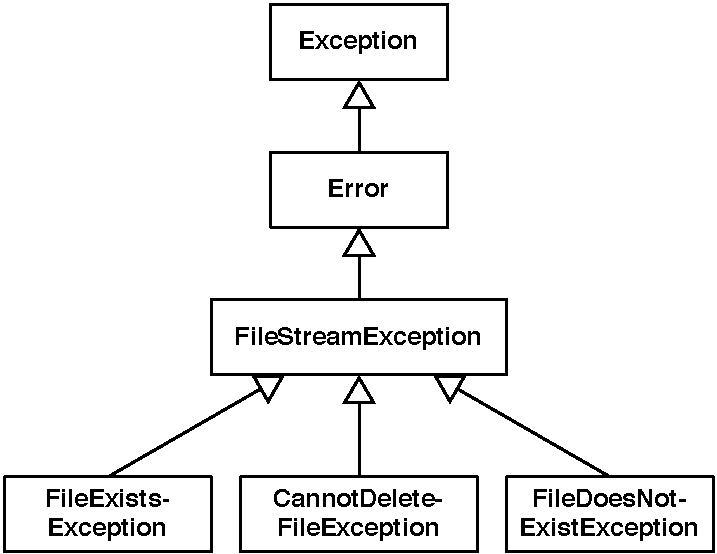
\includegraphics[width=.5\linewidth]{SimpleHierarchy}
        \caption{A small part of the \pharo exception hierarchy.\figlabel{hierarchy}}
\end{figure}


In \st, exceptions are, of course, objects. 
In \pharo{}, an exception is an instance of an exception class which is part of a hierarchy of exception classes.
For example, 
because the exceptions \clsind{FileDoesNotExistException}, \clsind{FileExistsException} and \clsind{CannotDeleteFileException} are special kinds of \clsind{FileStreamException}, they are represented as subclasses of \ct{FileStreamException}, as shown in \figref{hierarchy}.
This notion of ``specialization'' lets us associate an exception handler with a more or less general exceptional situation.
So, we can write:
\begin{code}{}
[ ... ] on: Error do: [ ... ]
[ ... ] on: FileStreamException do: [ ... ]
[ ... ] on: FileDoesNotExistException do: [ ... ]
\end{code}


The class \ct{FileStreamException} adds information to class \ct{Exception} to characterize the specific abnormal situation it describes. Specifically, \ct{FileStreamException} defines the \ct{fileName} instance variable, which contains the name of the file that signaled the exception. The root of the exception class hierarchy is \ct{Exception}, which is a direct subclass of \ct{Object}.

%In some versions of \pharo, \ct{Exception} has 10 direct subclasses and 103 indirect subclasses!
%\begin{code}{} % NB: Fragile -- should not be a test
%Exception subclasses size     --> 10
%Exception subclasses 	        --> {Error . IllegalResumeAttempt . Notification . ProgressInitiationException . Abort . UnhandledError . TestFailure . Halt . MCNoChangesException . RefactoringWarning}
%Exception allSubclasses size --> 103
%\end{code}
%\ab{I removed this because I added a new subsection that discusses the hierarchy more completely.}

Two key messages are involved in exception handling: \ct{on:do:}, which, as we have already seen, is sent to blocks to set an exception handler, and \ct{signal}, which is sent to subclasses of \ct{Exception} to signal that an exception has occurred.

%=================================================================
\section{Signaling an exception}

To signal an exception\footnote{Synonyms are to ``raise'' or to ``throw'' an exception. Since the vital message is called \lct{signal}, we use that terminology exclusively in this chapter.}, you only need to create an instance of the exception class, and to send it the message \ct{signal}, or \ct{signal:} with a textual description. The class \ct{Exception class} provides a convenience method \ct{signal}, which creates and signals an exception. So, here are two equivalent ways to signal a \clsind{ZeroDivide} exception:
\needlines{2}
\begin{code}{}
	ZeroDivide new signal.
	ZeroDivide signal.    "class-side convenience method does the same as above"
\end{code}

You may wonder why it is necessary to create an instance of an exception in order to signal it, rather than having the exception class itself take on this responsibility. Creating an instance is important because it encapsulates information about the context in which the exception was signaled. We can therefore have many exception instances, each describing the context of a different exception.

When an exception is signaled, the exception handling mechanism searches in the execution stack for an exception handler associated with the class of the signaled exception. When a handler is encountered (\ie the message \ct{on:do:} is on the stack),
the implementation checks that the \ct{exceptionClass} is a superclass of the signaled exception, and then executes the \ct{handlerAction} with the exception as its sole argument. We will see shortly some of the ways in which the handler can use the exception object.

When signaling an exception, it is possible to provide information specific to the situation just encountered, as illustrated in the code below. 
For example, if the file to be opened does not exist, the name of the non-existent file can be recorded in the exception object:

\mthindex{StandardFileStream class}{oldFileNamed:}
\begin{code}{}
StandardFileStream class>>>oldFileNamed: fileName
	"Open an existing file with the given name for reading and writing. If the name has no directory part, then default directory will be assumed. If the file does not exist, an exception will be signaled. If the file exists, its prior contents may be modified or replaced, but the file will not be truncated on close."
	| fullName |
	fullName := self fullName: fileName.
	^(self isAFileNamed: fullName)
		ifTrue: [self new open: fullName forWrite: true]
		ifFalse: ["File does not exist..."
			(FileDoesNotExistException new fileName: fullName) signal]
\end{code}

The exception handler may make use of this information to recover from the abnormal situation. The argument \ct{ex} in an exception handler \ct{[:ex | ...]} will be an instance of \ct{FileDoesNotExistException} or of one of its subclasses. Here the exception is queried for the filename of the missing file by sending it the message \ct{fileName}.

\begin{code}{}
| result |
result := [(StandardFileStream oldFileNamed: 'error42.log') contentsOfEntireFile]
	on: FileDoesNotExistException
	do: [:ex | ex fileName , ' not available'].
Transcript show: result; cr
\end{code}

Every exception has a default description that is used by the development tools to report exceptional situations in a clear and comprehensible manner. To make the description available, all exception objects respond to the message \ct{description}. Moreover, the default description can be changed by sending the message \lct{messageText:  \emph{aDescription}}, or by signaling the exception using \lct{signal: \emph{aDescription}}.

Another example of signaling occurs in the \ct{doesNotUnderstand:} mechanism, a pillar of the reflective capabilities of \st. Whenever an object is sent a message that it does not understand, the VM will (eventually) send it the message \ct{doesNotUnderstand:} with an argument representing the offending message. The default implementation of \ct{doesNotUnderstand:}, defined in class \ct{Object}, simply signals a \clsind{MessageNotUnderstood} exception, causing a debugger to be opened at that point in the execution.

The \ct{doesNotUnderstand:} method illustrates the way in which exception-specific information, such as the receiver and the message that is not understood, can be stored in the exception, and thus made available to the debugger.
\mthindex{Object}{doesNotUnderstand:}

\needlines{4}
\begin{code}{}
Object>>>doesNotUnderstand: aMessage 
	 "Handle the fact that there was an attempt to send the given message to the receiver but the receiver does not understand this message (typically sent from the machine when a message is sent to the receiver and no method is defined for that selector)."
	MessageNotUnderstood new 
		message: aMessage;
		receiver: self;
		signal.
	^ aMessage sentTo: self.
\end{code}

That completes our description of how exceptions are used.  The remainder of this chapter discusses how exceptions are implemented, and adds some details that are relevant only if you define your own exceptions.

%=================================================================


\section{How breakpoints are Implemented}

As we discussed in the Debugger chapter of \emph{Pharo By Example}, 
the usual way of setting a \ind{breakpoint} within a \st{} method is to insert the message-send \ct{self halt} into the code. The method \mthind{Object}{halt}, implemented in \ct{Object}, uses exceptions to open a debugger at the location of the breakpoint; it is defined as follows:

\needlines{6}
\begin{code}{}
Object>>>halt
	"This is the typical message to use for inserting breakpoints during 
	debugging. It behaves like halt:, but does not call on halt: in order to 
	avoid putting this message on the stack. Halt is especially useful when 
	the breakpoint message is an arbitrary one."
	Halt signal
\end{code}

\index{exception!resumable}
\clsind{Halt} is a direct subclass of \clsind{Exception}. A \ct{Halt} exception is \emph{resumable}, which means that it is possible to continue execution after a \ct{Halt} is signaled. 

\ct{Halt} overrides the \mthind{Halt}{defaultAction} method, which specifies the action to perform if the exception is not caught (\ie there is no exception handler for \ct{Halt} anywhere on the execution stack):

\begin{code}{}
Halt>>>defaultAction
	"No one has handled this error, but now give them a chance to decide
	how to debug it.  If no one handles this then open debugger
	(see UnhandedError-defaultAction)"
	UnhandledError signalForException: self
\end{code}

This code signals a new exception, \ct{UnhandledError}, that conveys the idea that no handler is present. The \ct{defaultAction} of \ct {UnhandledError} is to open a debugger:

\mthindex{UnhandledError}{defaultAction}
\begin{code}{}
UnhandledError>>>defaultAction
	"The current computation is terminated. The cause of the error should be logged or reported to the user. If the program is operating in an interactive debugging environment the computation should be suspended and the debugger activated."
	^ ToolSet debugError: exception.
\end{code}

\noindent
A few messages later, the debugger opens:

\mthindex{StandardToolSet}{debug:context:label:contents:fullView:}
\begin{code}{}
StandardToolSet>>>debug: aProcess context: aContext label: aString contents: contents fullView: aBool
	^ Debugger openOn: aProcess context: aContext label: aString contents: contents fullView: aBool
\end{code}

%=================================================================
\section{How handlers are found}

\index{exception!handler}
\index{activation context}
We will now take a look at how exception handlers are found and fetched from the execution stack when an exception is signaled. 
However, before we do this, we need to understand how the control flow of a program is internally represented in the virtual machine.

At each point in the execution of a program, the execution stack of the program is represented as a list of activation contexts. Each activation context represents a method invocation and contains all the information needed for its execution, namely its receiver, its arguments, and its local variables. It also contains a reference to the context that triggered its creation, \ie the activation context associated with the method execution that sent the message that created this context. In \pharo, the class \ct{MethodContext} models this information. 
The references between activation contexts link them into a chain: this chain of activation contexts \emph{is} \st's execution stack.

Actually, there are two kinds of activation context in \pharo: \ct{methodContext}s and \ct{blockContext}s: the latter are used to represent the execution of blocks.  They have a common superclass \ct{ContextPart}.  We will ignore this detail for now.

Suppose that we attempt to open a \ct{FileStream} on a non-existent file from a \ct{doIt}.
A \ct{FileDoesNotExistException} will be signaled, and the execution stack will contain \ct{MethodContext}s for \ct{doIt}, \ct{oldFileNamed:}, and \ct{signal}, as shown in \figref{stack}.

\begin{figure}[bth]\centering
        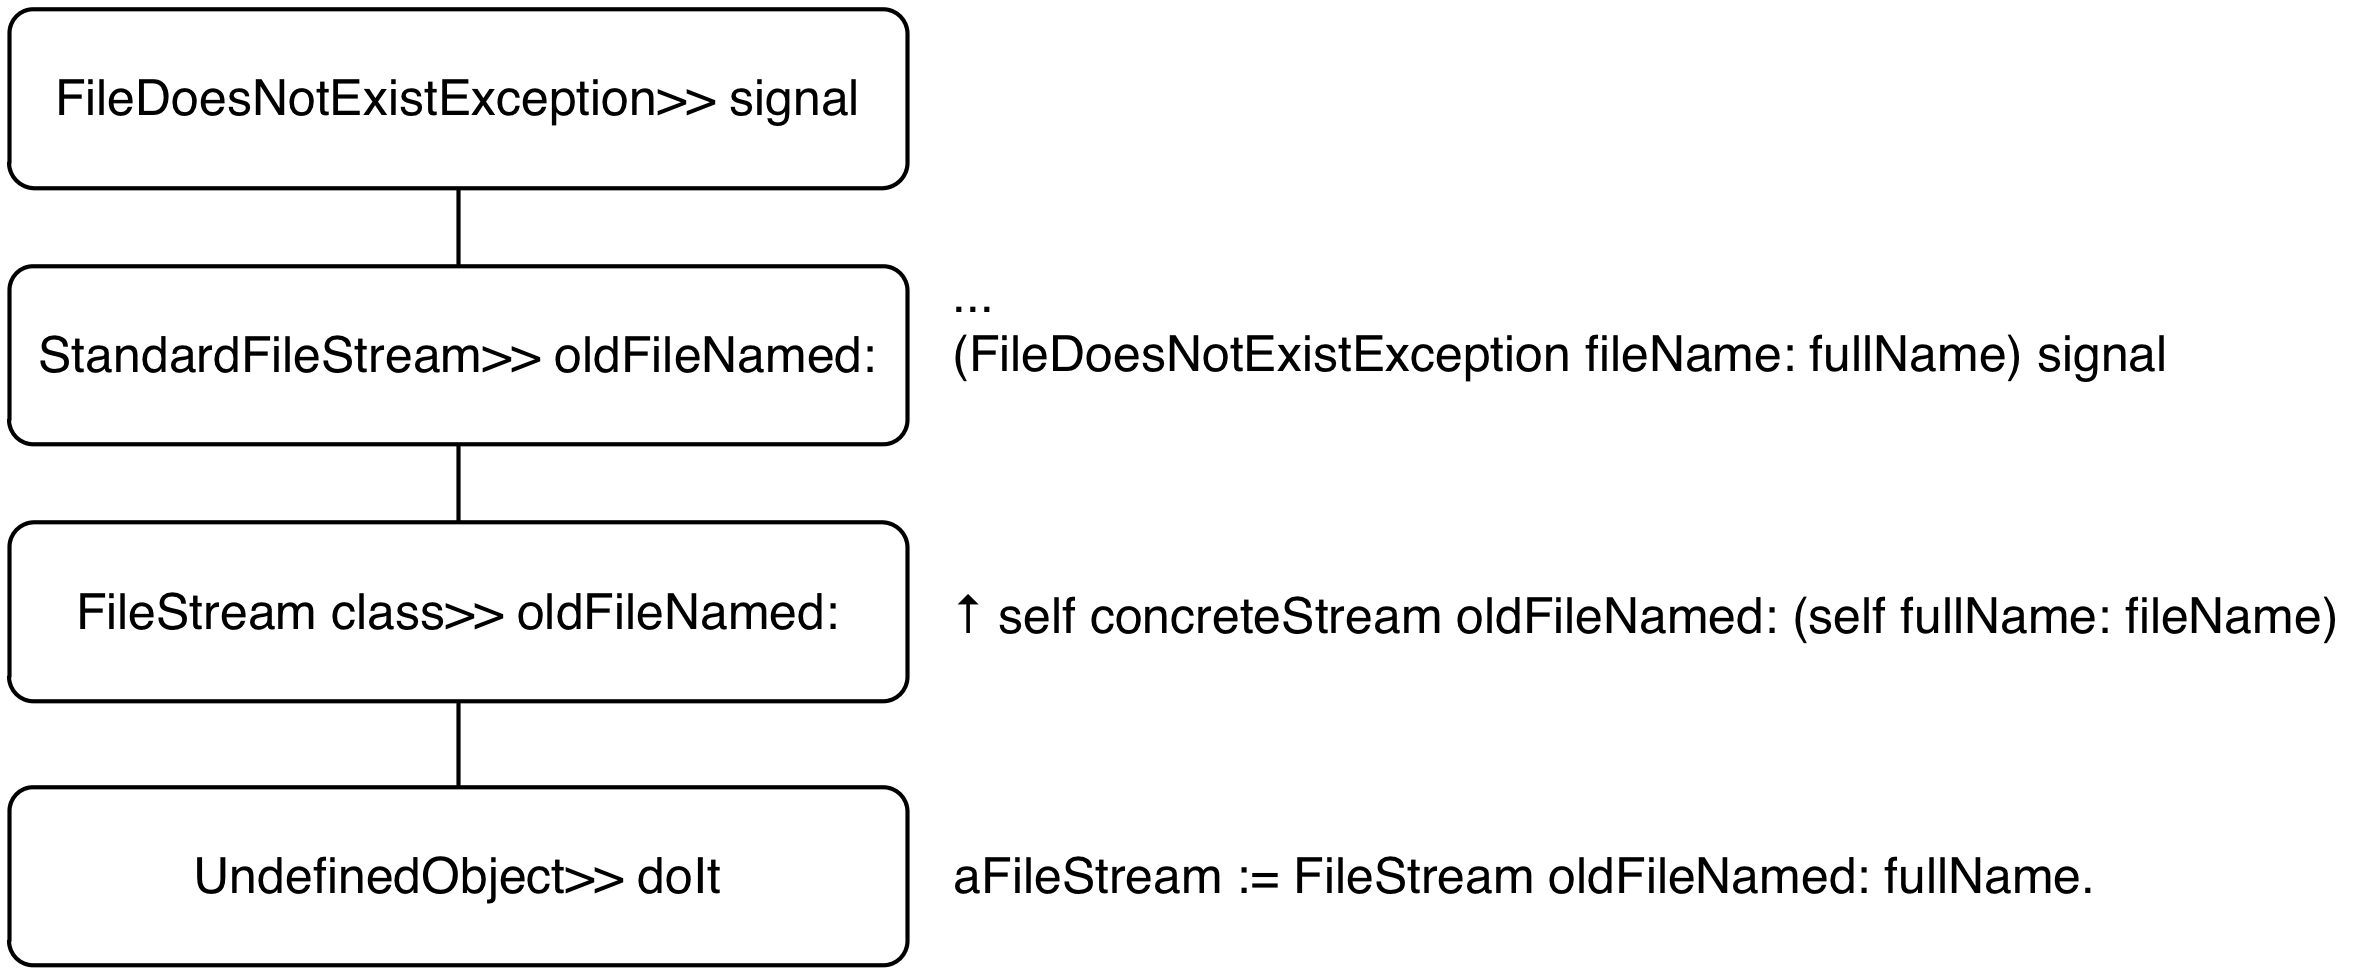
\includegraphics[width=\linewidth]{Stack}
        \caption{A \pharo execution stack.\figlabel{stack}}
\end{figure}

Since everything is an object in \st, we would expect method contexts to be objects.
However, some \st implementations use the native \ind{C} execution stack of the \ind{virtual machine} to avoid creating objects all the time.
The current \pharo virtual machine does actually use full Smalltalk objects all the time;  for speed, it recycles old method context objects rather than creating a new one for each message-send.

\index{BlockClosure!on:do:}
When we send \lct{\emph{aBlock} on: \emph{ExceptionClass} do: \emph{actionHandler}}, we intend to associate an exception handler (\lct{\emph{actionHandler}}) with a given class of exceptions (\lct{\emph{ExceptionClass}}) for the activation context of the protected block \lct{\emph{aBlock}}.
This information is used to identify and execute \lct{\emph{actionHandler}} whenever an exception of an appropriate class is signaled; \lct{\emph{actionHandler}} can be found by traversing the stack starting from the top (the most resent message-send) and working down to the context that sent the \ct{on:do:} message.

If there is no exception handler on the stack, the message \ct{defaultAction} will be sent either by \cmind{ContextPart}{handleSignal:} or by \cmind{UndefinedObject}{handleSignal:}. The latter is associated with the bottom of the stack, and is defined as follows:

\begin{code}{}
UndefinedObject>>>handleSignal: exception
	"When no more handler (on:do:) context is left in the sender chain, this gets called.  Return from signal with default action."
	^ exception resumeUnchecked: exception defaultAction
\end{code}

The message \ct{handleSignal:} is sent by \cmind{Exception}{signal}. 

When an exception $E$ is signaled, the system identifies and fetches the corresponding exception handler by searching down the stack as follows:

\begin{enumerate}

\item Look in the current activation context for a handler, and test if that handler \ct{canHandleSignal:} $E$.

\item If no handler is found and the stack is not empty, go down the stack and return to step 1.

\item If no handler is found and the stack is empty, then send \ct{defaultAction} to $E$. The default implementation in the \ct{Error} class leads to the opening of a debugger.

\item If the handler is found, send it \ct{value:} $E$.

\end{enumerate}

\paragraph{Nested Exceptions.}
Exception handlers are outside of their own scope.  This means that if an exception is signaled from within an exception handler\,---\,what we call a nested exception\,---\,a \emph{separate} handler must be set to catch the nested exception.

Here is an example where one \ct{on:do:} message is the receiver of another one; the second will catch errors signaled by the handler of the first:
\begin{code}{@TEST | result |}
result := [[ Error signal: 'error 1' ]
	on: Exception
	do: [ Error signal: 'error 2' ]]
		on: Exception
		do: [:ex | ex description ].
result --> 'Error: error 2'
\end{code}

Without the second handler, the nested exception will not be caught, and the debugger will be invoked.

An alternative would be to specify the second handler within the first one:
\needlines{5}
\begin{code}{@TEST | result |}
result := [ Error signal: 'error 1' ]
	on: Exception
	do: [[ Error signal: 'error 2' ]
		on: Exception
		do: [:ex | ex description ]].
result --> 'Error: error 2'
\end{code}

%=================================================================
\section{Handling exceptions}

\index{exception!handling}
When an exception is signaled, the handler has several choices about how to handle it.
In particular, it may:
\begin{itemize}
\item[(i)] \emph{abandon} the execution of the protected block, by simply specifying an alternative result;
\item[(ii)] \emph{return} an alternative result for the protected block, by sending \lct{return: \emph{aValue}} to the exception object;
\item[(iii)] \emph{retry} the protected block, by sending \ct{retry}, or try a different block by sending \ct{retryUsing:};
\item[(iv)] \emph{resume} the protected block at the failure point, by sending \ct{resume} or \ct{resume:};
\item[(v)] \emph{pass} the caught exception to the enclosing handler, by sending \ct{pass}; or
\item[(vi)] \emph{resignal} a different exception, by sending \ct{resignalAs:} to the exception.
% \lr{I would call this \emph{resignal}, because this is not the same as signaling a new exception using \ct{Exception signal} from within a handler block.}
\end{itemize}

We will briefly look at the first three possibilities, and then we will take a closer look at the remaining ones.

%-----------------------------------------------------------------
\subsection{Abandon the protected block}

The first possibility is to abandon the execution of the protected block, as follows:
\needlines{7}
\begin{code}{@TEST |answer|}
answer := [ |result|
	result := 6 * 7.
	Error signal.
	result 	"This part is never evaluated"
]	on: Error
	do: [ :ex | 3 + 4 ].
answer --> 7
\end{code}

The handler takes over from the point where the error is signaled, and any code following in the original block is not evaluated.

%-----------------------------------------------------------------
\subsection{Return a value with \ct{return:}}
A block returns the value of the last statement in the block, regardless of whether the block is protected or not. However, there are some situations where the result needs to be returned by the handler block. The message \lct{return: \emph{aValue}} sent to an exception has the effect of returning \lct{\emph{aValue}} as the value of the protected block:

\begin{code}{@TEST |result|}
result := [Error signal]
	on: Error
	do: [ :ex | ex return: 3 + 4 ].
result --> 7
\end{code}

The \ind{ANSI standard} is not clear regarding the difference between using \ct{do: [:ex | 100 ]} and \ct{do: [:ex | ex return: 100]} to return a value. We suggest that you use \mthind{Exception}{return:} since it is more intention-revealing, even if these two expressions are equivalent in \pharo.

A variant of \ct{return:} is the message \ct{return}, which returns \ct{nil}. 

Note that, in any case, control will \emph{not} return to the protected block, but will be passed on up to the enclosing context.

\begin{code}{@TEST}
6 * ([Error signal] on: Error do: [ :ex | ex return: 3 + 4 ]) --> 42
\end{code}

%-----------------------------------------------------------------
\subsection{Retry a computation with \ct{retry} and \ct{retryUsing:}}

\index{exception!retrying}
Sometimes we may want to change the circumstances that led to the exception and retry the protected block. This is done by sending \mthind{Exception}{retry} or \mthind{Exception}{retryUsing:} to the exception object. It is important to be sure that the conditions that caused the exception have been changed before retrying the protected block, or else an infinite  loop will result:
\begin{code}{}
[Error signal] on: Error do: [:ex | ex retry]    "will loop endlessly"
\end{code}

Here is a better example.
The protected block is re-evaluated within a modified environment where \ct{theMeaningOfLife} is properly initialized:
\begin{code}{@TEST | result theMeaningOfLife |}
result := [ theMeaningOfLife * 7 ]    "error -- theMeaningOfLife is nil"
	on: Error
	do: [:ex | theMeaningOfLife := 6. ex retry ].
result --> 42
\end{code}

The message \ct{retryUsing: aNewBlock} enables the protected block to be replaced by \ct{aNewBlock}. This new block is executed and is protected with the same handler as the original block.

\begin{code}{@TEST | x result |}
x := 0.
result := [ x/x ]    "fails for x=0"
	on: Error
	do: [:ex |
		x := x + 1.
		ex retryUsing: [1/((x-1)*(x-2))]    "fails for x=1 and x=2"
	].
result --> (1/2)    "succeeds when x=3"
\end{code}

The following code loops endlessly:
\begin{code}{}
[1 / 0] on: ArithmeticError do: [:ex | ex retryUsing: [ 1 / 0 ]]
\end{code}
whereas this will signal an \ct{Error}: 
\begin{code}{}
[1 / 0] on: ArithmeticError do: [:ex | ex retryUsing: [ Error signal ]]
\end{code}

As another example, recall the file handling code we saw earlier, in which we printed a message to the Transcript when a file is not found. Instead, we could prompt for the file as follows:
\begin{code}{}
[(StandardFileStream oldFileNamed: 'error42.log') contentsOfEntireFile]
	on: FileDoesNotExistException
	do: [:ex | ex retryUsing: [FileList modalFileSelector contentsOfEntireFile] ]
\end{code}

%=================================================================
\section{Resuming execution}

\index{exception!resuming execution}
A method that signals an exception that \ct{isResumable} can be resumed at the place immediately following the signal. An exception handler may therefore perform some action, and then resume the execution flow. This behavior is achieved by sending \mthind{Exception}{resume:} to the exception in the handler.
The argument is the value to be used in place of the expression that signaled the exception.
In the following example we signal and catch \ct{MyResumableTestError}, which is defined in the Tests-Exceptions category:

\begin{code}{}
result := [ | log |
	log := OrderedCollection new.
	log addLast: 1.
	log addLast: MyResumableTestError signal. 
	log addLast: 2.
	log addLast: MyResumableTestError signal.
	log addLast: 3.
	log ] 
		on: MyResumableTestError 
		do: [ :ex |  ex resume: 0 ].
result --> an OrderedCollection(1 0 2 0 3)
\end{code}
Here we can clearly see that the value of \ct{MyResumableTestError signal} is the value of the argument to the \ct{resume:} message.

The message \ct{resume} is equivalent to \ct{resume: nil}.

The usefulness of resuming an exception is illustrated by the class \ct{Installer}, which implements an automatic package loading mechanism. When installing packages, warnings may be signaled. Warnings should not be considered fatal errors, so the installer should simply ignore the warning and continue installing. \lr{Maybe better use something from Pharo-Core like \ct{UndeclaredVariableWarning} or \ct{TimedOut}.}
\ab{St\'{e}ph and I failed to find a better example.  If you have one, go ahead and replace this one.}

\begin{code}{}
Installer>>>installQuietly: packageNameCollectionOrDetectBlock 
	self package: packageNameCollectionOrDetectBlock. 
	 [ self install ] on: Warning do: [ :ex | ex resume ]. 
\end{code}
%	 [ self install ] on: Warning do: [ :ex | ex resume: true ]. 
% The code actually says resume: true, but Keith Hodges confirms that this is not necessary

Another situation where resumption is useful is when you want to ask the user what to do.  For example, suppose that we were to define a class \ct{ResumableLoader} with the following method:
\begin{code}{}
ResumableLoader>>>readOptionsFrom: aStream 
	| option |
	[aStream atEnd]
		whileFalse: [option := self parseOption: aStream.
			"nil if invalid"
			option isNil
				ifTrue: [InvalidOption signal]
				ifFalse: [self addOption: option]].
	aStream close
\end{code}
\noindent
If an invalid option is encountered, we signal an \ct{InvalidOption} exception.
The context that sends \ct{readOptionsFrom:} can set up a suitable handler:

\begin{code}{}
ResumableLoader>>>readConfiguration
	| stream |
	stream := self optionStream.
	[self readOptionsFrom: stream]
		on: InvalidOption
		do: [:ex | (UIManager default confirm: 'Invalid option line. Continue loading?')
				ifTrue: [ex resume]
				ifFalse: [ex return]].
	stream close
\end{code}

\noindent
Depending on user input, the handler in \ct{readConfiguration} might \ct{return} \ct{nil}, or it might \ct{resume} the exception, causing the \ct{signal} message send in \ct{readOptionsFrom:} to return and the parsing of the options stream to continue.

Note that \ct{InvalidOption} must be resumable; it suffices to define it as a subclass of \ct{Exception}.

%=================================================================
\subsection{Example: Deprecation}

\index{deprecation (pattern)}
\emph{Deprecation} offers a case study of a mechanism built using resumable exceptions.
Deprecation is a software re-engineering pattern that allows us to mark a method as being ``deprecated'', meaning that it may disappear in a future release and should not be used by new code.
In \pharo, a method can be marked as deprecated as follows:

\mthindex{Object}{deprecated:}
\begin{code}{}
Utilities class>>>convertCRtoLF: fileName
	"Convert the given file to LF line endings. Put the result in a file with the extention '.lf'"

	self deprecated: 'Use ''FileStream convertCRtoLF: fileName'' instead.' 
		on: '10 July 2009' in: #Pharo1.0 .
	FileStream convertCRtoLF: fileName
\end{code}

When the message \ct{convertCRtoLF:} is sent, if the \ct{raiseDeprecationWarnings} preference is  \ct{true}, then a pop-up window is displayed with a notification and the programmer may resume the application execution; this is shown in \figref{deprecation}.


\begin{figure}[ht]\centering
        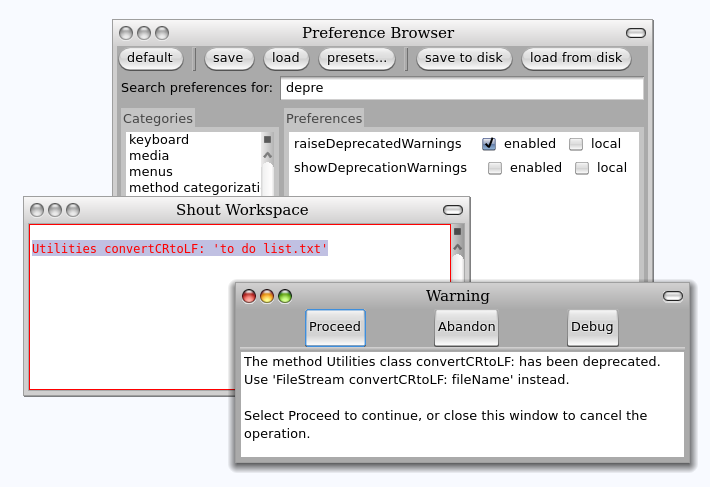
\includegraphics[width=\linewidth]{Deprecation}
        \caption{Sending a deprecated message.\figlabel{deprecation}}
\end{figure}

Deprecation is implemented in \pharo in just a few steps.
First, we define \clsind{Deprecation} as a subclass of \clsind{Warning}.
It should have some instance variables to contain information about the deprecation: in 
\pharo{} these are \ct{methodReference}, \ct{explanationString}, \ct{deprecationDate} and \ct{versionString}; we therefore need to define an instance-side initialization method for these variables, and a class-side instance creation method that sends the corresponding message.

When we define a new exception class, we should consider overriding \ct{isResumable}, \ct{description}, and \ct{defaultAction}.
In this case the inherited implementations of the first two methods are fine:

\begin{itemize}
\item \ct{isResumable} is inherited from \clsind{Exception}, and answers \ct{true};
\item \ct{description} is inherited from \ct{Exception}, and answers an adequate textual description.
\end{itemize}

However, it is necessary to override the implementation of \lct{defaultAction}, because we want that to depend on some preferences.  Here is \pharo's implementation:
\begin{code}{}
Deprecation>>>defaultAction
	Log ifNotNil: [:log| log add: self].
	Preferences showDeprecationWarnings ifTrue:
		[Transcript nextPutAll: explanationString; cr; flush].
	Preferences raiseDeprecatedWarnings ifTrue:
		[super defaultAction]
\end{code}

The first preference simply causes a warning message to be written on the \ct{Transcript}.  The second preference asks for an exception to be signaled, which is accomplished by \super-sending \ct{defaultAction}.

We also need to implement some convenience methods in \ct{Object}, like this one:
\needlines{8}
\begin{code}{}
Object>>>deprecated: anExplanationString on: date in: version
	(Deprecation
		method: thisContext sender method
		explanation: anExplanationString
		on: date
		in: version) signal
\end{code}

%=================================================================
\section{Passing exceptions on}

To illustrate the remaining possibilities for handling exceptions, we will look at how to implement a generalization of the \ct{perform:} method.
If we send \lct{perform: \emph{aSymbol}} to an object, this will cause the message named \lct{\emph{aSymbol}} to be sent  to that object:
\begin{code}{@TEST}
5 perform: #factorial --> 120    "same as: 5 factorial"
\end{code}

Several variants of this method exist. For example:
\begin{code}{@TEST}
1 perform: #+ withArguments: #(2) --> 3    "same as: 1 + 2"
\end{code}
These \ct{perform:}-like methods are very useful for accessing an interface dynamically, since the messages to be sent can be determined at run-time.

One message that is missing is one that will send a cascade of unary messages to a given receiver. A simple and naive implementation is:
\begin{code}{}
Object>>>performAll: selectorCollection
	selectorCollection do: [:each | self perform: each]    "aborts on first error"
\end{code}

This method could be used as follows:
\begin{code}{}
Morph new performAll: #( #activate #beTransparent #beUnsticky)
\end{code}

However, there is a complication. There might be a selector in the collection that the object does not understand (such as \ct{#activate}). We would like to ignore such selectors and continue sending the remaining messages. The following implementation seems to be reasonable:

\needlines{4}
\begin{code}{}
Object>>>performAll: selectorCollection 
	selectorCollection do: [:each |
		[self perform: each]
			on: MessageNotUnderstood
			do: [:ex | ex return]]    "also ignores internal errors"
\end{code}

On closer examination we notice another problem. This handler will not only catch and ignore messages not understood by the original receiver, but also any messages sent but not understood in methods for messages that \emph{are} understood! This will hide programming errors in those methods, which is not our intent.
To fix this, we need our handler to analyze the exception to see if it was indeed caused by the attempt to perform the current selector.
Here is the correct implementation.
\begin{method}[objectPerformAll]{Object>>performAll:}
Object>>>performAll: selectorCollection 
	selectorCollection do: [:each | 
		[self perform: each] 
			on: MessageNotUnderstood 
			do: [:ex | (ex receiver == self and: [ex message selector == each]) 
				ifTrue: [ex return] 
				ifFalse: [ex pass]]]    "pass internal errors on"
\end{method}

This has the effect of passing on \clsind{MessageNotUnderstood} errors to the surrounding context when they are not part of the list of messages we are performing. The \ct{pass} message will pass the exception on to the next applicable handler in the execution stack.

If there is no next handler on the stack, the \ct{defaultAction} message is sent to the exception instance. The \ct{pass} action does not modify the sender chain in any way\,---\,but the handler that control is passed to may do so. Like the other messages discussed in this section, \ct{pass} is special\,---\,it never returns to the sender.

The goal of this section has been to demonstrate the power of exceptions.
It should be clear that while you can do almost anything with exceptions, the code
that results not is always easy to understand.   
There is often a simpler way to get he same effect without exceptions; see \mthref{simplerObjectPerfromAll} on page \pageref{mth:simplerObjectPerfromAll} for a better way to implement \ct{performAll:}.

%=================================================================
\section{Resending exceptions}

\index{exception!resending}
Now suppose that in our \ct{performAll:} example we no longer want to ignore selectors not understood by the receiver, but instead we want to consider an occurrence of such a selector as an error. However, we want it to be signaled as an application-specific exception, let's say \ct{InvalidAction}, rather than the generic \ct{MessageNotUnderstood}. In other words, we want the ability to ``resignal'' a signaled exception as a different one.

It might seem that the solution would simply be to signal the new exception in the handler block. The handler block in our implementation of \ct{performAll:} would be:

\mthindex{Exception}{pass}
\begin{code}{}
[:ex | (ex receiver == self and: [ex message selector == each])
	ifTrue: [InvalidAction signal]    "signals from the wrong context"
	ifFalse: [ex pass]]
\end{code}

A closer look reveals a subtle problem with this solution, however. Our original intent was to replace the occurrence of \ct{MessageNotUnderstood} with \ct{InvalidAction}. This replacement should have the same effect as if \lct{InvalidAction} were signaled at the same place in the program as the original \ct{MessageNotUnderstood} exception. Our solution signals \ct{InvalidAction} in a different location. The difference in locations may well lead to a difference in the applicable handlers.

To solve this problem, resignaling an exception is a special action handled by the system. For this purpose, the system provides the message \lct{resignalAs:}. The correct implementation of a handler block in our \ct{performAll:} example would be:

\begin{code}{}
 [:ex |  (ex receiver == self and: [ex message selector == each])
	ifTrue: [ex resignalAs: InvalidAction]    "resignals from original context"
	ifFalse: [ex pass]]
\end{code}

%=================================================================
\section{Comparing \lct{outer} with \lct{pass}}

The method \mthind{Exception}{outer} is very similar to \ct{pass}. Sending \ct{outer} to an exception also evaluates the enclosing handler action. The only difference is that if the outer handler resumes the exception, then control will be returned to the point where \ct{outer} was sent, not the original point where the exception was signaled:

\begin{code}{@TEST | passResume |}
passResume := [[ Warning signal . 1 ]    "resume to here"
	on: Warning
	do: [ :ex | ex pass . 2 ]]
		on: Warning
		do: [ :ex | ex resume ].
passResume --> 1    "resumes to original signal point"
\end{code}

\needlines{6}
\begin{code}{@TEST | outerResume |}
outerResume := [[ Warning signal . 1 ]
	on: Warning
	do: [ :ex | ex outer . 2 ]]    "resume to here"
		on: Warning
		do: [ :ex | ex resume ].
outerResume --> 2    "resumes to where outer was sent"
\end{code}

%=================================================================
\section{Catching sets of exceptions}

So far we have always used \ct{on:do:} to catch just a single class of exception. The handler will only be invoked if the exception signaled is a sub-instance of the specified exception class.
However, we can imagine situations where we might like to catch multiple classes of exceptions. This is easy to do:

\begin{code}{@TEST | result |}
result := [ Warning signal . 1/0 ]
	on: Warning, ZeroDivide
	do: [:ex | ex resume: 1 ].
result --> 1
\end{code}

If you are wondering how this works, just have a look at the implementation of \ct{Exception class>>>,}

\begin{code}{}
Exception class>>>, anotherException
	"Create an exception set."

	^ExceptionSet new
		add: self;
		add: anotherException;
		yourself
\end{code}

The rest of the magic occurs in the class \clsind{ExceptionSet}, which has a surprisingly trivial implementation.

\begin{code}{}
Object subclass: #ExceptionSet
	instanceVariableNames: 'exceptions'
	classVariableNames: ''
	poolDictionaries: ''
	category: 'Exceptions-Kernel'

ExceptionSet>>>initialize
	super initialize.
	exceptions := OrderedCollection new

ExceptionSet>>>, anException
	self add: anException.
	^self

ExceptionSet>>>add: anException
	exceptions add: anException

ExceptionSet>>>handles: anException
	exceptions do: [:ex | (ex handles: anException) ifTrue: [^true]].
	^false
\end{code}

\noindent
\ab{Is there some reason that \ct{ExceptionSet>>>handles:} isn't implemented using \ct{anySatisfy:}?}

%=========================================================
\section{How exceptions are implemented}

%\on{As an explanation, this part really does not work. I would prefer to leave it out.}
%\sd{no this is really important I did a new pass on it}

Let's have a look at how exceptions are implemented at the Virtual Machine level.

%\on{need new intro}

%\ugh{Up to now, we have presented the use of exceptions in \st without really saying a word about their implementation.
%at the execution engine level (Virtual Machine). 
%Normally you do not need to know how handlers are really looked up at execution time to use exceptions.
%Therefore in the first reading you can skip this section. Now if you are curious and really want to know how this is implemented at the Virtual Machine level, this section is for you. 
%This section will uncover the internal of the Pharo exception mechanism.
%The mechanism is quite simple, making it worth to know how it operates.
%This section is a wonderful example on how Pharo can reveal information just by browsing its source code.}


\paragraph{Storing Handlers.}
First we need to understand how the exception class and its associated handler  are stored and how this information is found at run-time. 
Let's look at the definition of the central method \mthind{BlockClosure}{on:do:} defined on the class \ct{BlockClosure}. % which is the class representing the block-closure. 

\mthindex{BlockClosure}{on:do:}
\needlines{6}
\begin{code}{}
BlockClosure>>>on: exception do: handlerAction 
	"Evaluate the receiver in the scope of an exception handler." 
	| handlerActive | 
	<primitive: 199> 
	handlerActive := true. 
	^self value 
\end{code}

This code tells us two things: First, this method is implemented as a primitive, which means that  a primitive operation of the virtual machine is executed when this method is invoked.  VM primitives don't normally return: successful execution of a primitive terminates the method that contains the \lct{<primitive: \emph{n}\,>} instruction, answering the result of the primitive.
So, the \st code that follows the primitive serves two purposes: it documents what the primitive does, and is available to be executed if the primitive should fail. 
Here we see that \ct{on:do:} simply sets the temporary variable \ct{handlerActive} to true, and then evaluates the receiver (which is, of course, a block).  

This is surprisingly simple, but somewhat puzzling.  Where are the arguments of the \ct{on:do:} method stored?  Let's look at the definition of the class \ct{MethodContext}, whose instances make up the execution stack: 

\begin{code}{}
ContextPart variableSubclass: #MethodContext
	instanceVariableNames: 'method closureOrNil receiver'
	classVariableNames: ''
	poolDictionaries: ''
	category: 'Kernel-Methods'
\end{code}

There is no instance variable here to store the exception class or the handler, nor is there any place  in the superclass to store them. 
However, note that \ct{MethodContext} is defined as a \ct{variableSubclass}.
This means that in addition to the named instance variables, objects of this class have some numbered slots.  In fact, every \ct{MethodContext} has a numbered slot for each  argument of the method whose invocation it represents.  There are also additional numbered slots for the temporary variables of the method.

To verify this, you can evaluate the following piece of code:

\begin{code}{}
| exception handler | 
[exception := thisContext sender at: 1. 
 handler := thisContext sender at: 2. 
 1 / 0] 
on: Error 
do: [:ex| ]. 
{ exception . handler } explore
\end{code}

The last line explores a 2-element array that contains the exception class and the exception handler. 

\paragraph{Finding Handlers.}
Now that we know where the information is stored, let's have a look at how it is found at runtime. 

We might think that the primitive 199 is complex to write. 
But it too is trivial, because primitive 199 \emph{always} fails!
Because the primitive always fails, the \st{} body of \ct{on:do:} is always executed.
However, the presence of the \ct{<primitive 199>} bytecode marks the executing context in a unique way. 

The source code of the primitive is found in \ct{Interpreter>>>primitiveMarkHandlerMethod} in the \pkgind{VMMaker} \sqsrc project: 

\begin{code}{}
primitiveMarkHandlerMethod
     "Primitive. Mark the method for exception handling. The primitive must fail after
     marking the context so that the regular code is run."
     
     self inline: false.
    ^self primitiveFail
\end{code}
\hyphenation{Method-Context}
So now we know that when the method \ct{on:do:} is executed, the \ct{MethodContext} that makes up the stack frame is tagged and the handler and exception class 
are stored there. 

Now, if an exception is signaled further up the stack, the method \ct{signal} can search the stack to find the appropriate handler:

\mthindex{Exception}{signal}
\needlines{5}
\begin{code}{}
Exception>>>signal
	"Ask ContextHandlers in the sender chain to handle this signal.
	The default is to execute and return my defaultAction."

	signalContext := thisContext contextTag.
	^ thisContext nextHandlerContext handleSignal: self
\end{code}

\mthindex{Exception}{nextHandlerContext}
\begin{code}{}
ContextPart>>>nextHandlerContext

	^ self sender findNextHandlerContextStarting
\end{code}

The method \ct{findNextHandlerContextStarting} is implemented as a primitive (number 197); its body describes what it does. It looks to see
if the stack frame is a context created by the execution of the method \ct{on:do:} (it just looks to see if the primitive number is 199). If this is the case it answers with that context. 

\mthindex{MethodContext}{findNextHandlerContextStarting}
\begin{code}{}
ContextPart>>>findNextHandlerContextStarting 
	"Return the next handler marked context, returning nil if there 
	is none. Search starts with self and proceeds up to nil." 
	| ctx |	
	<primitive: 197> 
	ctx := self. 
	[  ctx isHandlerContext ifTrue: [^ctx]. 
	   (ctx := ctx sender) == nil ] whileFalse. 
	^nil 
\end{code}

\begin{code}{}
MethodContext>>>isHandlerContext 
	"is this context for method that is marked?" 
	^method primitive = 199 
\end{code}

Since the method context supplied by \ct{findNextHandlerContextStarting} contains all the exception-handling information, it can be examined to see if the exception class is suitable for handling the current exception.
If so, the associated handler can be executed; if not, the look-up can continue further. 
This is all implemented in the \ct{handleSignal:} method.

\begin{code}{}
ContextPart>>>handleSignal: exception
	"Sent to handler (on:do:) contexts only.  If my exception class (first arg) handles exception then execute my handle block (second arg), otherwise forward this message to the next handler context.  If none left, execute exception's defaultAction (see nil>>handleSignal:)."

	| val |
	(((self tempAt: 1) handles: exception) and: [self tempAt: 3]) ifFalse: [
		^ self nextHandlerContext handleSignal: exception].

	exception privHandlerContext: self contextTag.
	self tempAt: 3 put: false.  "disable self while executing handle block"
	val := [(self tempAt: 2) valueWithPossibleArgs: {exception}]
		ensure: [self tempAt: 3 put: true].
	self return: val.  "return from self if not otherwise directed in handle block"
\end{code}

Notice how this method uses \ct{tempAt: 1} to access the exception class, and ask if it handles the exception.   What about  \ct{tempAt: 3}?  That is the temporary variable \ct{handlerActive} of the \ct{on:do:} method.   Checking that \ct{handlerActive} is \ct{true} and then setting it to \ct{false} ensures that a handler will not be asked to handle an exception that it signals itself. 
The \ct{return:} message sent as the final action of \ct{handleSignal} is responsible for ``unwinding'' the execution stack by removing the stack frames above \self{}.

The full story is only slightly more complicated because there are actually two classes of objects that make up the stack, \ct{MethodContext}s, which we have already discussed, and \ct{BlockContext}s, which represent the execution of blocks.  \ct{ContextPart} is their common superclass.

So, to summarize, the \ct{signal} method, with minimal assistance from the virtual machine, finds the context that correspond to an \ct{on:do:} message with an appropriate exception class.   Because the execution stack is made up of Context objects that may be manipulated just like any other object, the stack can be shortened at any time.  This is a superb example of flexibility of \st.

%=========================================================
\section{Other kinds of Exception}

The class \ct{Exception} in \pharo{} has ten direct subclasses, as shown in \figref{wholeHierarchy}.
The first thing that we notice from this figure is that the Exception hierarchy is a bit of a mess; you can expect to see some of the details change as \pharo{} is improved.

\begin{figure}[ht]\centering
        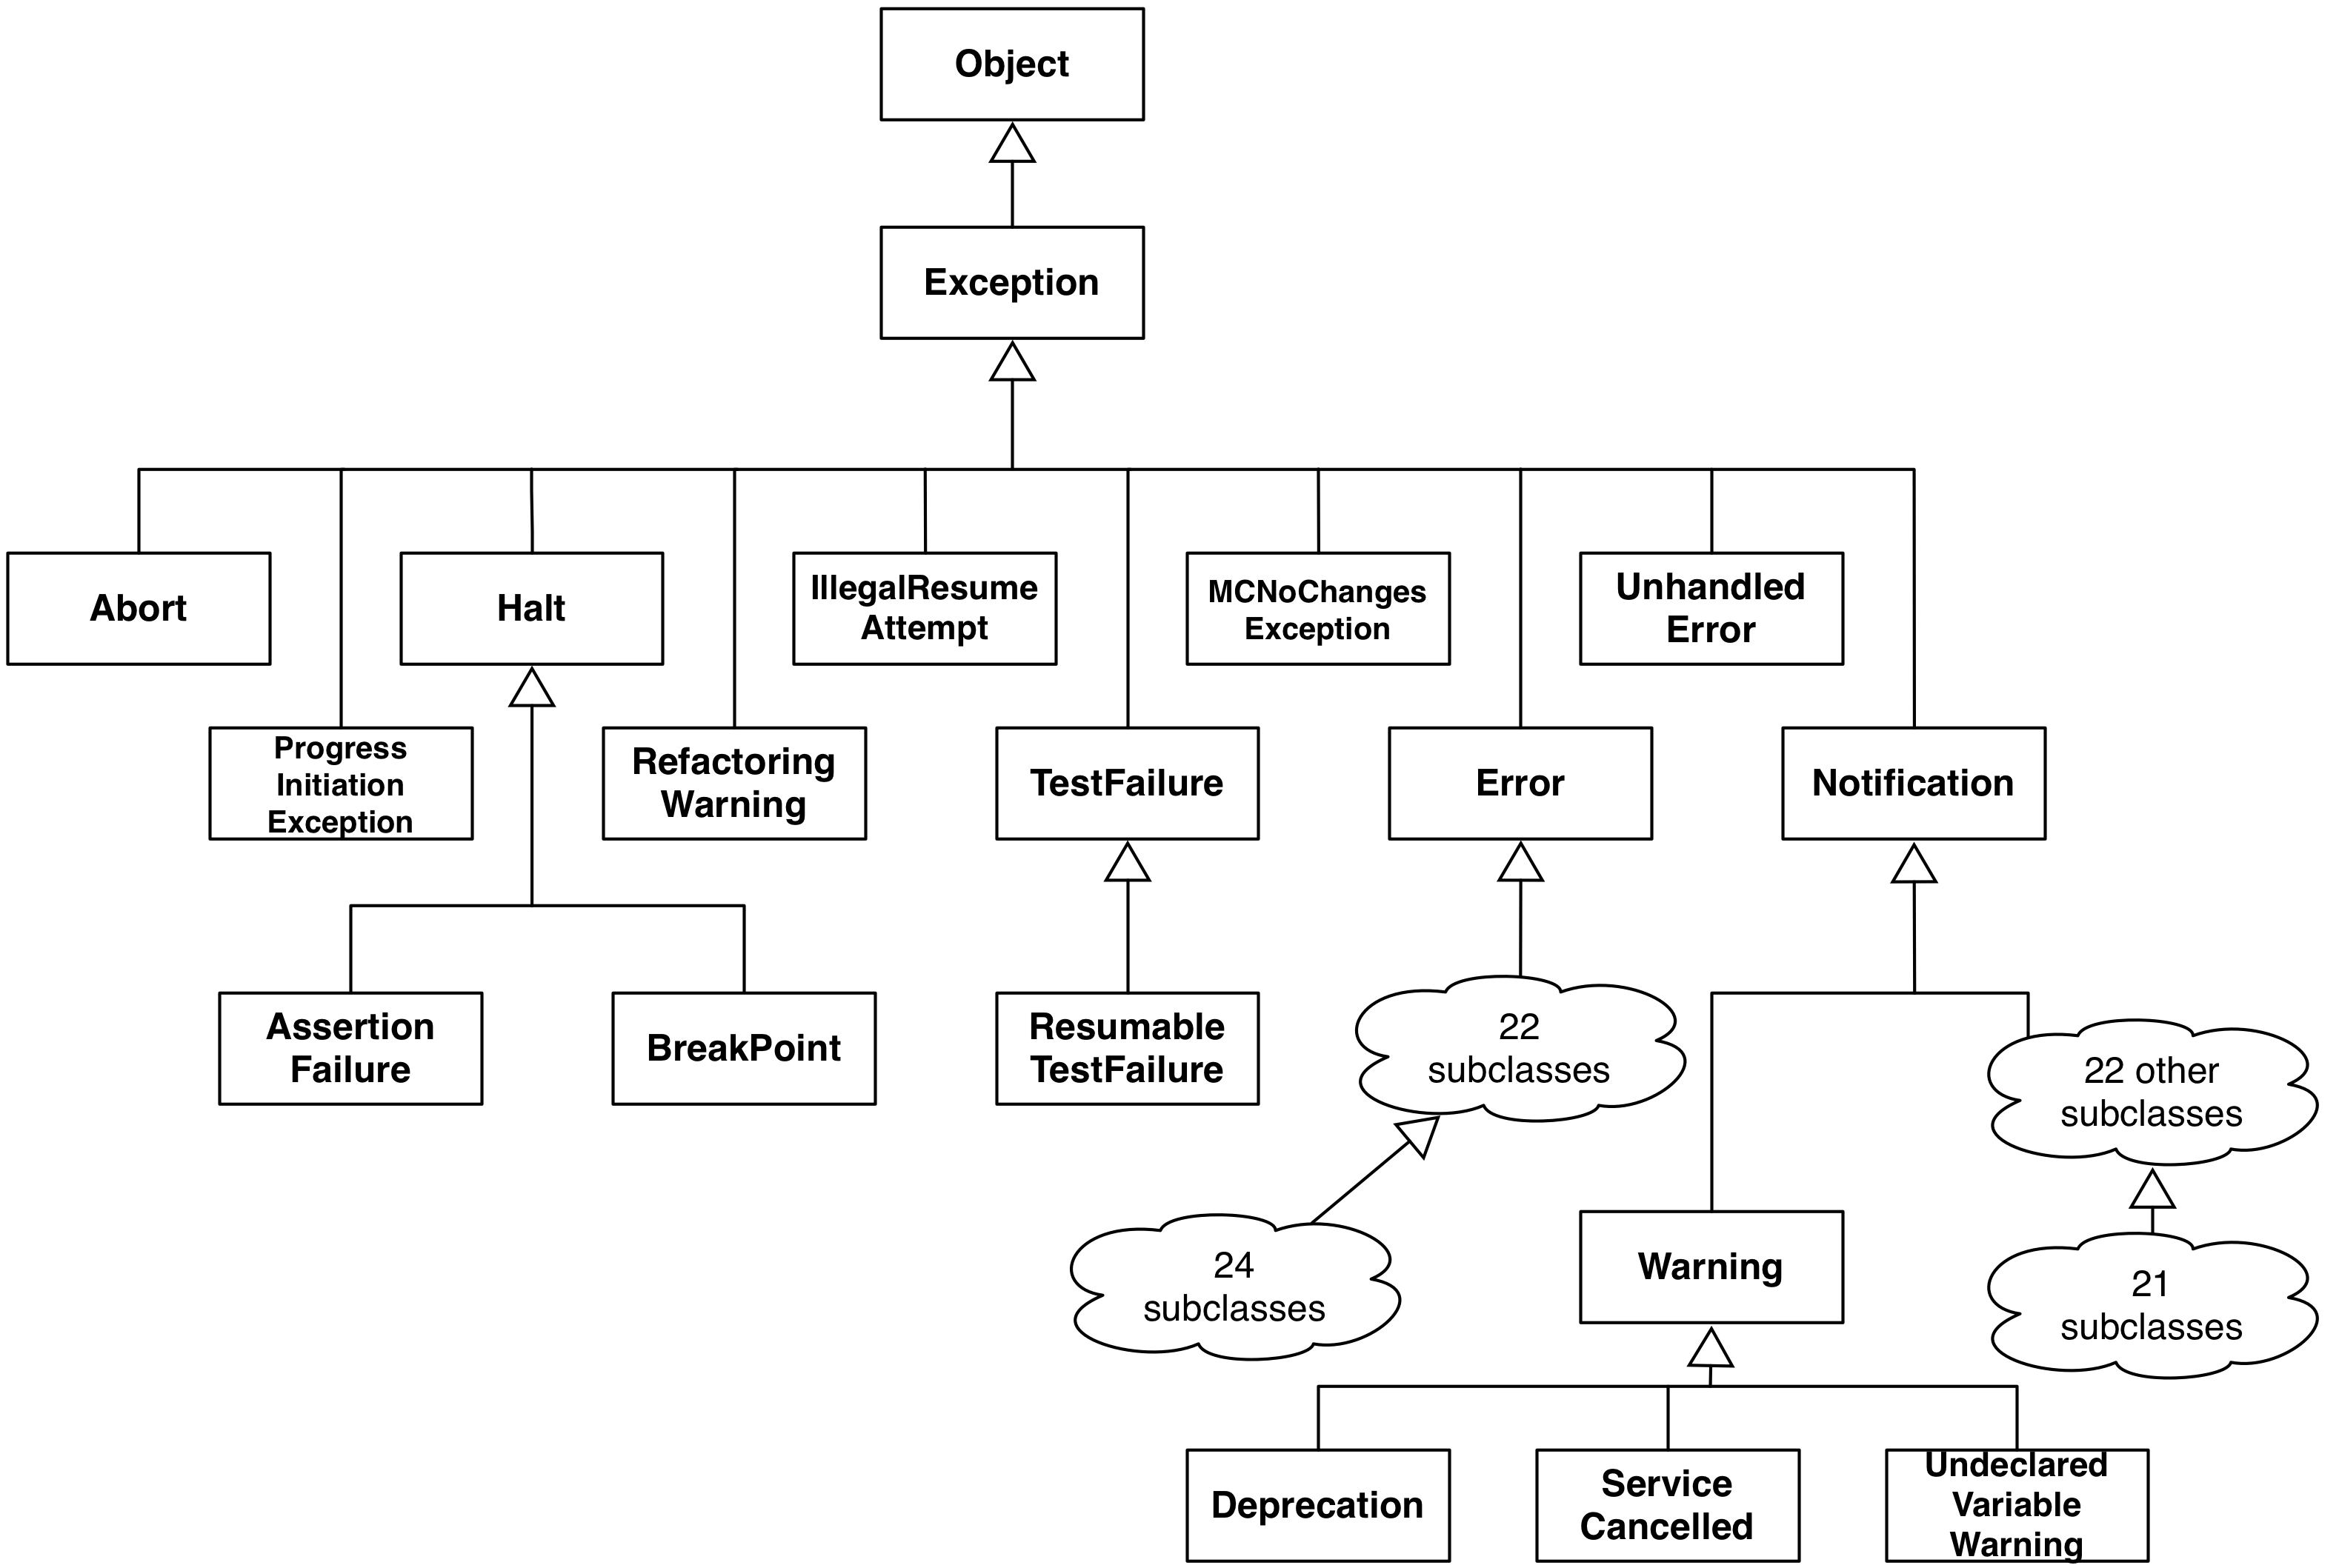
\includegraphics[width=.95\linewidth]{ExceptionSubclasses}
        \caption{The whole \pharo exception hierarchy.\figlabel{wholeHierarchy}}
\end{figure}

The second thing that we notice is that there are two large sub-hierarchies: \ct{Error} and \ct{Notification}. 
Errors tell us that the program has fallen into some kind of abnormal situation. 
In contrast, Notifications tell us that an event has occurred, but without the assumption that it is abnormal. 
So, if a \ct{Notification} is not handled, the program will continue to execute. 
An important subclass of \ct{Notification} is \ct{Warning};  warnings are used to notify other parts of the system, or the user, of abnormal but non-lethal behavior.
%
%Graphical user interfaces make great use of notifications. In \pharo, \ct{ProgressNotification}, another subclass of \ct{Notification}, is used to move the progress bar forward when a long-running task is being executed. \ab{I wanted to put in a reference to the methods that do this, but couldn't find them.  Can someone else put this in, please?} 
%\ab{This appears not to be true, so I commented out the whole paragraph}

The property of being resumable is largely orthogonal to the location of an exception in the hierarchy.   In general, \ct{Error}s are not resumable, but 10 of its subclasses \emph{are} resumable.  For example, \ct{MessageNotUnderstood} is a subclass of \ct{Error}, but it is resumable.  \ct{TestFailure}s are not resumable, but, as you would expect, \ct{ResumableTestFailure}s are. 

Resumability is controlled by the private \ct{Exception} method \mthind{Exception}{isResumable}. 
For example:
\begin{code}{@TEST}
Exception new isResumable --> true
Error new isResumable --> false
Notification new isResumable --> true
Halt new isResumable --> true
MessageNotUnderstood new isResumable --> true
\end{code}

As it turns out, roughly 2/3 of all exceptions are resumable:
\begin{code}{}
Exception allSubclasses size --> 103
(Exception allSubclasses select: [:each | each new isResumable]) size --> 66
\end{code}
If you declare a new subclass of exceptions, you should look in its protocol for the \ct{isResumable} method, and override it as appropriate to the semantics of your exception.

In some situations, it will never makes sense to resume an exception.
In such a case you should signal a non-resumable subclass\,---\,either an existing one or one of your own creation.
In other situations, it will always be OK to resume an exception, without the handler having to do anything.
In fact, this gives us another way of characterizing a notification:
a \ct{Notification} is a resumable \ct{Exception} that can be safely resumed them without first modifying the state of the system.
More often, it will be safe to resume an exception only if the state of the system is first modified in some way.
So, if you signal a resumable exception, you should be very clear about what you expect an exception handler to do before it resumes the exception.

\section{When not to use Exceptions}
Just because \pharo{} has exception handling, you should not conclude that it is always appropriate to use it.  
Recall that in the introduction to this chapter, we said that exception handling is for \emph{exceptional} situations.  
So, the first rule for using exceptions is \emph{not} to use them for situations that \emph{can reasonably be expected to occur} in a normal execution. 

Of course, if you are writing a library, what is normal depends on the context in which your library is used.
To make this concrete, let's look at \ct{Dictionary} as an example:
\lct{\emph{aDictionary} at: \emph{aKey}} will signal an \ct{Error} if \lct{\emph{aKey}} is not present.
But you should not write a handler for this error!
If the logic of your application is such that there is some possibility that the key will not be in the dictionary, then you should instead use \lct{at: \emph{aKey} ifAbsent: [\emph{remedial action}]}.
In fact, \ct{Dictionary>>>at:} is implemented using \ct{Dictionary>>>at:ifAbsent:}.
\lct{\emph{aCollection} detect: \emph{aPredicateBlock}} is similar: if there is any possibility that the predicate might not be satisfied, you should use \lct{\emph{aCollection} detect: \emph{aPredicateBlock} ifNone: [\emph{remedial action}]}. 

When you write methods that signal exceptions, you should consider whether you should also provide an alternative method that takes a remedial block as an additional argument, and evaluates it if the normal action cannot be completed.  
Although this technique can be used in any programming language that support closures, because \st{} uses closures for \emph{all} its control structures, it is a particularly natural one to use in \st{}.

Another way of avoiding exception handling is to test the precondition of the exception before sending the message that may signal it.  For example, in \mthref{objectPerformAll}, we sent a message to an object using \ct{perform:}, and handled the \ct{MessageNotUnderstood} error that might ensue.  A much simpler alternative is to check to see if the message is understood before executing the \ct{perform:}

\needlines{5}
\begin{method}[simplerObjectPerfromAll]{Object>>performAll: revisited}
performAll: selectorCollection
	selectorCollection
		do: [:each | (self respondsTo: each)
				ifTrue: [self perform: each]]
\end{method}

The primary objection to \mthref{simplerObjectPerfromAll} is efficiency.  The implementation of \ct{respondsTo: s} has to lookup \ct{s} in the target's method dictionary  to find out if \ct{s} will be understood.  If the answer is yes, then \ct{perform:} will look it up again.  Moreover, the first lookup is implemented in \st, not in the virtual machine.  If this code is in a performance-critical loop, this might be an issue.  However, if the collection of messages comes from a user interaction, the speed of \ct{performAll:} will not be a problem.

%=================================================================
\section{Chapter Summary}

In this chapter we saw how to use exceptions to signal and handle abnormal situations arising in our code.

\begin{itemize}
\item Don't use exceptions as a control-flow mechanism.  Reserve them for notifications and for \emph{abnormal} situations.  Consider providing methods that take blocks as arguments as an alternative to signaling exceptions.

\item Use \lct{\emph{protectedBlock} ensure: \emph{actionBlock}} to ensure that \lct{\emph{actionBlock}} will be performed even if \lct{\emph{protectedBlock}} terminates abnormally.

\item Use \lct{\emph{protectedBlock} ifCurtailed: \emph{actionBlock}} to ensure that \lct{\emph{actionBlock}} will be performed \emph{only} if \lct{\emph{protectedBlock}} terminates abnormally.

\item Exceptions are objects. Exceptions classes form a hierarchy with the class \ct{Exception} at the root of the hierarchy.

\item Use \lct{\emph{protectedBlock} on: \emph{ExceptionClass} do: \emph{handlerBlock}} to catch exceptions that are instances of \lct{\emph{ExceptionClass}} (or any of its subclasses). The \lct{\emph{handlerBlock}} should take an exception instance as its sole argument.

\item Exceptions are signaled by sending one of the messages \lct{signal} or \lct{signal:}. \ct{signal:} takes a descriptive string as its argument. The description of an exception can be obtained by sending it the message \ct{description}.

\item You can set a breakpoint in your code by inserting the message-send \ct{self halt}. This signals a resumable \ct{Halt} exception, which, by default, will open a debugger at the point where the breakpoint occurs.

\item When an exception is signaled, the runtime system will search up the execution stack, looking for a handler for that specific class of exception. If none is found, the \ct{defaultAction} for that exception will be performed (\ie in most cases the debugger will be opened).

\item An exception handler may terminate the protected block by sending \ct{return:} to the signaled exception; the value of the protected block will be the argument supplied to \ct{return:}. 

\item An exception handler may retry a protected block by sending \ct{retry} to the signaled exception. The handler remains in effect.

\item An exception handler may specify a new block to try by sending \ct{retryUsing:} to the signaled exception, with the new block as its argument. Here, too, the handler remains in effect.

\item Notifications are subclass of Exception with the property that they can be safely resumed without the handler having to take any specific action.

\end{itemize}

\paragraph{Acknowledgments.}  We gratefully acknowledge Vassili Bykov for the raw material he provided. We also thank Paolo Bonzini, the main developer of GNU \st, for the \st implementations of \ct{ensure:} and \ct{ifCurtailed:}.
\index{Bonzini, Paolo}
\index{GNU \st}

%=========================================================
\ifx\wholebook\relax\else
   \bibliographystyle{jurabib}
   \nobibliography{scg}
   \end{document}
\fi
%=========================================================

